\documentclass[11pt,oneside]{report}

% =========================================================
% PACKAGES
% =========================================================
\usepackage[margin=0.80in,top=0.80in,bottom=0.80in]{geometry}
\usepackage{lmodern}
\usepackage[T1]{fontenc}
\usepackage{amsmath,amssymb,amsfonts}
\usepackage{graphicx}
\usepackage{booktabs,tabularx,multirow,longtable}
\usepackage{listings}
\usepackage{float}
\usepackage{algorithm}
\usepackage{algpseudocode}
\usepackage{fancyhdr}
\usepackage{titlesec}
\usepackage{caption}
\usepackage{subcaption}
\usepackage{microtype}
\usepackage{setspace}
\usepackage{color,xcolor}
\usepackage{pdfpages}
\usepackage{tikz}
\usetikzlibrary{shapes.geometric, arrows, arrows.meta, positioning, calc}
\usepackage[pdftex,bookmarksnumbered=true,colorlinks=true,linkcolor=black,citecolor=black,urlcolor=black]{hyperref}
\usepackage{bookmark}

% =========================================================
% DOCUMENT METADATA
% =========================================================
\hypersetup{
    pdftitle={Machine-Learning-Driven Implied Volatility Forecasting and Relative Option Valuation: An Empirical Study on NIFTY 50 Weekly Index Options},
    pdfauthor={Diviya C.},
    pdfsubject={Corporate Internship Report (MSQF 534)},
    pdfkeywords={Implied Volatility, Black-Scholes-Merton, Random Forest, XGBoost, Persistence Benchmark, Option Valuation, Scenario Stress Testing, Expiry Day Regime Shift, NIFTY 50 Options}
}

% =========================================================
% GRAPHICS PATH
% =========================================================
\graphicspath{{figures/}{./}}

% =========================================================
% CUSTOM COLORS & LISTINGS STYLING
% =========================================================
\definecolor{codegreen}{rgb}{0,0.6,0}
\definecolor{codegray}{rgb}{0.5,0.5,0.5}
\definecolor{codeblue}{rgb}{0,0,0.8}
\definecolor{backgroundcolor}{rgb}{0.97,0.97,0.97}
\definecolor{charcoal}{rgb}{0.2,0.2,0.2}
\definecolor{headergray}{rgb}{0.7,0.7,0.7}
\definecolor{commentgray}{rgb}{0.5,0.5,0.5}

% Currency Command
\newcommand{\rupee}{\text{Rs.\ }}

\lstset{
    backgroundcolor=\color{backgroundcolor},
    commentstyle=\color{codegreen},
    keywordstyle=\color{codeblue}\bfseries,
    numberstyle=\tiny\color{codegray},
    stringstyle=\color{codegreen},
    basicstyle=\ttfamily\footnotesize,
    breakatwhitespace=false,
    breaklines=true,
    captionpos=b,
    keepspaces=true,
    numbers=left,
    numbersep=5pt,
    showspaces=false,
    showstringspaces=false,
    showtabs=false,
    tabsize=2
}

% =========================================================
% LAYOUT & HEADER/FOOTER CONFIGURATIONS
% =========================================================
\setstretch{1.10}
\pagestyle{fancy}
\fancyhf{}
\fancyhead[L]{\textcolor{charcoal}{\small\nouppercase{\leftmark}}}
\fancyhead[R]{\textcolor{charcoal}{\small\thepage}}
\renewcommand{\headrule}{\hbox to\headwidth{\color{headergray}\leaders\hrule height 0.4pt\hfill}}
\renewcommand{\chaptermark}[1]{\markboth{#1}{}}
\setlength{\headheight}{24pt}
\addtolength{\topmargin}{-14pt}

% Float Spacing Refinements
\setlength{\floatsep}{8pt plus 2pt minus 2pt}
\setlength{\textfloatsep}{10pt plus 2pt minus 2pt}
\setlength{\intextsep}{8pt plus 2pt minus 2pt}
\setlength{\abovecaptionskip}{4pt plus 1pt minus 1pt}
\setlength{\belowcaptionskip}{4pt plus 1pt minus 1pt}

% Algorithmic Styling Refinements
\renewcommand{\algorithmiccomment}[1]{\hfill\textcolor{commentgray}{\ensuremath{\triangleright}\ \textit{#1}}}

% Chapter Title Spacing
\titleformat{\chapter}[display]
  {\normalfont\large\bfseries}{\chaptername\ \thechapter}{4pt}{\Large}
\titlespacing*{\chapter}{0pt}{-14pt}{10pt}
\titlespacing*{\section}{0pt}{8pt}{4pt}
\titlespacing*{\subsection}{0pt}{6pt}{3pt}

% Paragraph Spacing
\setlength{\parskip}{0.3em}
\setlength{\parindent}{1.3em}

% Float Layout Optimization
\renewcommand{\topfraction}{0.9}
\renewcommand{\bottomfraction}{0.8}
\renewcommand{\textfraction}{0.05}
\renewcommand{\floatpagefraction}{0.85}

\begin{document}

% =========================================================
% TITLE PAGE
% =========================================================
\hypersetup{pageanchor=false}
\begin{titlepage}
    \begin{center}
        \vspace*{0.2cm}
        
        \textbf{\large PONDICHERRY UNIVERSITY} \\[0.2cm]
        \textbf{\large RAMANUJAN SCHOOL OF MATHEMATICAL SCIENCES} \\[0.2cm]
        \textbf{\large DEPARTMENT OF STATISTICS} \\[0.35cm]
        
        
\includegraphics[width=0.22\textwidth]{pondicherry_university_logo} \\[0.35cm]
        
        \textbf{\large M.Sc. QUANTITATIVE FINANCE} \\[0.2cm]
        \textbf{\large MSQF 534: Corporate Internship} \\[0.2cm]
        \textbf{\large REPORT ON} \\[0.35cm]
        
        \textbf{\Large Machine-Learning-Driven Implied Volatility Forecasting \& Relative Option Valuation} \\[0.25cm]
        {\large An Empirical Study on NIFTY 50 Weekly Index Options \par}
        \vspace{0.6cm}
        
        \textbf{\large SUBMITTED BY} \\[0.4cm]
        
        \textbf{\large NAME: DIVIYA C.} \\[0.2cm]
        \textbf{\large REG. NO.: 25MSQUFPY0018} \\[0.6cm]
        
        \textbf{\large UNDER THE GUIDANCE OF} \\[0.2cm]
        \textbf{\normalsize Surabhi Investment Services Pvt. Ltd., Tiruchirappalli, Tamil Nadu} \\[0.7cm]
        
        \textbf{\large NOVEMBER 2026}
        
    \end{center}
\end{titlepage}

\hypersetup{pageanchor=true}
\pagenumbering{roman}
\pagestyle{plain}

% =========================================================
% UNIVERSITY CERTIFICATE PAGE
% =========================================================
\newpage
\thispagestyle{plain}
\phantomsection
\addcontentsline{toc}{chapter}{University Certificate}
\begin{center}
    
\includegraphics[width=0.20\textwidth]{pondicherry_university_logo} \\[0.3cm]
    \textbf{\large PONDICHERRY UNIVERSITY} \\[0.15cm]
    \textbf{\large RAMANUJAN SCHOOL OF MATHEMATICAL SCIENCES} \\[0.15cm]
    \textbf{\large DEPARTMENT OF STATISTICS} \\[0.4cm]
    
    \textbf{\large CERTIFICATE} \\[0.6cm]
\end{center}

\noindent
Certified to be the bonafide record of work done in \textbf{MSQF 534: Corporate Internship} by \underline{\textbf{DIVIYA C.\vphantom{Q}}} with Register No. \underline{\textbf{25MSQUFPY0018}} of class \textbf{II M.Sc. Quantitative Finance} in the Department of Statistics, Ramanujan School of Mathematical Sciences, Pondicherry University, Puducherry -- 605 014, during the academic year 2026--2027.

\vspace{1.5cm}
\noindent
\begin{minipage}{0.45\textwidth}
    \begin{flushleft}
        \rule{4.5cm}{0.4pt} \\
        \textbf{Faculty - in - charge}
    \end{flushleft}
\end{minipage}
\hfill
\begin{minipage}{0.45\textwidth}
    \begin{flushright}
        \rule{4.5cm}{0.4pt} \\
        \textbf{Head / Coordinator}
    \end{flushright}
\end{minipage}

\vspace{1.2cm}
\noindent
\textbf{Date:}

\vspace{1.2cm}
\noindent
\textbf{Submitted for the M.Sc. Degree Practical Examination held on \rule{4cm}{0.4pt}.}

\vspace{1.0cm}
\hfill
\begin{minipage}{0.45\textwidth}
    \begin{flushright}
        \rule{4.5cm}{0.4pt} \\
        \textbf{Examiners}
    \end{flushright}
\end{minipage}

% =========================================================
% COMPANY INTERNSHIP CERTIFICATE
% =========================================================
\newpage
\thispagestyle{plain}
\phantomsection
\addcontentsline{toc}{chapter}{Company Internship Certificate}
\begin{center}
    \vspace*{0.3cm}
    \textbf{\LARGE SURABHI INVESTMENT SERVICES PVT. LTD.} \\[0.2cm]
    \textbf{\large Quantitative Research \& Financial Derivatives Division} \\[0.1cm]
    \textbf{\small Tiruchirappalli, Tamil Nadu, India} \\[0.5cm]
    \rule{\textwidth}{1.2pt} \\[0.8cm]
    
    \textbf{\Large CERTIFICATE OF INTERNSHIP COMPLETION} \\[0.8cm]
\end{center}

\noindent
This is to certify that \textbf{Ms. DIVIYA C.} (Register No. \textbf{25MSQUFPY0018}), a student of \textbf{M.Sc. Quantitative Finance}, Department of Statistics, Pondicherry University, has successfully completed her corporate internship project titled:

\begin{center}
    \vspace{0.2cm}
    \textbf{\large ``Machine-Learning-Driven Implied Volatility Forecasting \& Relative Option Valuation''}
    \vspace{0.2cm}
\end{center}

\noindent
at \textbf{Surabhi Investment Services Pvt. Ltd.}, Tiruchirappalli, Tamil Nadu.

\vspace{0.5cm}
\noindent
During the tenure of her internship, she demonstrated outstanding technical proficiency, analytical acumen, and rigorous quantitative problem-solving capabilities in financial econometrics, machine learning architectures, automated market data harvesting, and derivatives valuation. Her research contributed significantly to our options desk modeling frameworks, specifically in 5-minute ahead implied volatility forecasting, Black-Scholes scenario analysis, and expiry-day regime risk diagnostics.

\vspace{0.5cm}
\noindent
Her conduct and work ethics during the project were exemplary. We wish her all success in her future academic and professional endeavors.

\vspace{2.2cm}
\noindent
\begin{minipage}{0.45\textwidth}
    \begin{flushleft}
        \rule{4.5cm}{0.4pt} \\
        \textbf{Managing Director / Research Head} \\
        Surabhi Investment Services Pvt. Ltd.
    \end{flushleft}
\end{minipage}
\hfill
\begin{minipage}{0.45\textwidth}
    \begin{flushright}
        \rule{4.5cm}{0.4pt} \\
        \textbf{Project Mentor} \\
        Quantitative Derivatives Desk
    \end{flushright}
\end{minipage}

% If a scanned copy is available, uncomment:
% \includepdf[pages=1,pagecommand={\thispagestyle{plain}\phantomsection\addcontentsline{toc}{chapter}{Internship Certificate}}]{internship_certificate.pdf}

% =========================================================
% DECLARATION & ACKNOWLEDGEMENTS
% =========================================================
\newpage
\thispagestyle{plain}
\phantomsection
\addcontentsline{toc}{chapter}{Declaration \& Acknowledgements}
\begin{center}
    \textbf{\Large DECLARATION} \\[0.4cm]
\end{center}

\noindent
I, \textbf{DIVIYA C.}, hereby declare that the corporate internship report titled \textbf{``Machine-Learning-Driven Implied Volatility Forecasting \& Relative Option Valuation: An Empirical Study on NIFTY 50 Weekly Index Options''} submitted to the Department of Statistics, Ramanujan School of Mathematical Sciences, Pondicherry University, in partial fulfillment of the requirements for the award of the degree of \textbf{Master of Science in Quantitative Finance}, is a record of original analytical work carried out by me under the institutional mentorship of \textbf{Surabhi Investment Services Pvt. Ltd.}, Tiruchirappalli, Tamil Nadu.

\vspace{0.3cm}
\noindent
\begin{minipage}{0.4\textwidth}
    \small
    \textbf{Place:} Puducherry \\
    \textbf{Date:} November 2026
\end{minipage}
\hfill
\begin{minipage}{0.55\textwidth}
    \begin{flushright}
        \small
        \textbf{DIVIYA C.} (Reg. No.: 25MSQUFPY0018) \\
        Department of Statistics, Pondicherry University
    \end{flushright}
\end{minipage}

\vspace{0.6cm}
\begin{center}
    \textbf{\Large ACKNOWLEDGEMENTS} \\[0.4cm]
\end{center}

\noindent
I express my deepest gratitude to the Almighty for the guidance and perseverance to complete this research. I express my profound gratitude to the quantitative research leadership and mentors at \textbf{Surabhi Investment Services Pvt. Ltd.}, Tiruchirappalli, Tamil Nadu, for their invaluable domain mentorship in derivatives trading and market making. 

\vspace{0.25cm}
\noindent
I extend my sincere appreciation to the \textbf{Head of the Department of Statistics} and the \textbf{Faculty Coordinator of M.Sc. Quantitative Finance}, Ramanujan School of Mathematical Sciences, Pondicherry University, as well as all esteemed faculty members, for their steadfast academic guidance. Finally, I dedicate this work to my beloved family and peers for their endless encouragement.

\vspace{0.4cm}
\hfill
\textbf{DIVIYA C.}

% =========================================================
% ABSTRACT
% =========================================================
\newpage
\thispagestyle{plain}
\phantomsection
\addcontentsline{toc}{chapter}{Abstract}
\begin{center}
    \textbf{\LARGE ABSTRACT} \\[0.8cm]
\end{center}

\noindent
Implied Volatility (IV) constitutes the market's forward-looking gauge of aggregate risk and the core unobservable input in options pricing and risk management. In high-frequency and intraday algorithmic derivatives trading, conventional market-making models frequently assume that implied volatility is stationary over short horizons (the \textit{persistence assumption}, $\widehat{\text{IV}}_{t+5} = \text{IV}_t$) or rely on static parametric volatility smiles. In reality, short-term volatility displays non-linear autoregressive clustering, asymmetric momentum responses to underlying spot moves, and market microstructure frictions. 

This thesis presents the design, mathematical formulation, empirical benchmarking, and production deployment of an end-to-end quantitative machine learning framework for **5-minute-ahead implied volatility forecasting ($\Delta \text{IV}_{t+5}$)** and **relative option valuation** on **NIFTY 50 weekly index options** traded on the National Stock Exchange of India (NSE). The framework ingests regularized 5-minute option chain snapshots via the Upstox API v2, enforces rigorous data hygiene (filtering non-positive IV quotes, invalid bid-ask spreads, and near-ATM strike constraints $0.95 \le K/S \le 1.05$), calculates exact fractional Time-to-Expiry (TTE) in hours, and engineers a 39-dimensional feature space capturing multi-horizon volatility velocity, spot momentum, and order book liquidity.

Using a strict chronological train/test split to prevent look-ahead bias, predictive models are empirically evaluated against the random walk persistence benchmark and an Ordinary Least Squares (OLS) linear baseline. A tuned Random Forest regressor engineered with short-term volatility lags achieves a **5.28\% reduction in Mean Absolute Error (MAE)** (0.5214 vs.\ 0.5505) and a **7.72\% reduction in Root Mean Squared Error (RMSE)** (1.2188 vs.\ 1.3207) over the persistence baseline, while OLS completely deteriorates ($R^2 = -0.2410$, $\text{MAE} = 6.1720$) due to extreme non-linear curvature across moneyness space. Gini importance metrics reveal that recent volatility velocity ($\text{IV}_{\text{change}, 5m}$, $\text{IV}_{\text{change}, 10m}$) and bid-ask spreads dominate static contract characteristics. Applying directional conviction thresholding ($|\widehat{\Delta \text{IV}}| \ge 0.10$) increases directional classification accuracy from a noisy baseline of **53.20\% to 63.40\%** (and 64.47\% at $\ge 0.25$), providing execution desks with actionable filter mechanics.

The forecasted volatility is synthesized into a Relative IV Valuation Engine, categorizing option strikes into **Fair/Neutral (77.92\%)**, **Overvalued/Rich (15.46\%)**, and **Undervalued/Cheap (6.61\%)** regimes to drive systematic spread strategies. A multi-factor Black-Scholes scenario engine evaluates non-linear Greek sensitivities across joint spot, volatility, and time shocks. Crucially, out-of-sample stress testing on an unseen weekly expiry day (October 19, 2026, $T < 1.58$ hours) reveals an econometric regime breakdown ($\text{MAE}$ spiking to 17.42), proving that non-expiry volatility dynamics collapse in the hyper-gamma, hyper-theta, vanishing-vega final hours. Finally, the system is operationalized via a live 5-minute automated background prediction daemon and an institutional multi-page Streamlit analytics dashboard.

% =========================================================
% TABLE OF CONTENTS & LISTS
% =========================================================
\newpage
\phantomsection
\addcontentsline{toc}{chapter}{Table of Contents}
\setcounter{tocdepth}{1}
\tableofcontents

\newpage
\phantomsection
\addcontentsline{toc}{chapter}{Lists of Figures, Tables \& Abbreviations}
\begin{center}
    \textbf{\Large List of Figures}
\end{center}
\vspace{-0.2cm}
\makeatletter
\@starttoc{lof}
\makeatother

\vspace{0.3cm}
\begin{center}
    \textbf{\Large List of Tables}
\end{center}
\vspace{-0.2cm}
\makeatletter
\@starttoc{lot}
\makeatother

\vspace{0.3cm}
\begin{center}
    \textbf{\Large List of Abbreviations} \\[0.15cm]
    \scriptsize
    \renewcommand{\arraystretch}{0.85}
    \begin{tabular}{ll@{\qquad}ll}
        \toprule
        \textbf{Abbrev.} & \textbf{Full Form} & \textbf{Abbrev.} & \textbf{Full Form} \\
        \midrule
        \textbf{API} & Application Programming Interface & \textbf{LTP} & Last Traded Price \\
        \textbf{ATM} & At-The-Money & \textbf{MAE} & Mean Absolute Error \\
        \textbf{BSM} & Black-Scholes-Merton & \textbf{MSE} & Mean Squared Error \\
        \textbf{CE} & European Call Option & \textbf{NSE} & National Stock Exchange of India \\
        \textbf{GARCH} & Generalized Autoregressive Cond. Het. & \textbf{OI} & Open Interest \\
        \textbf{GBM} & Geometric Brownian Motion & \textbf{OLS} & Ordinary Least Squares \\
        \textbf{IST} & Indian Standard Time (UTC+05:30) & \textbf{PCR} & Put-Call Ratio \\
        \textbf{ITM} & In-The-Money & \textbf{PE} & European Put Option \\
        \textbf{IV} & Implied Volatility & \textbf{RF} & Random Forest \\
        \textbf{LOB} & Limit Order Book & \textbf{RMSE} & Root Mean Squared Error \\
        \textbf{NIFTY} & National Stock Exchange Fifty Index & \textbf{TTE} & Time-to-Expiry \\
        \textbf{OTM} & Out-Of-The-Money & \textbf{XGBoost} & eXtreme Gradient Boosting \\
        \bottomrule
    \end{tabular}
\end{center}

% =========================================================
% MAIN TEXT CHAPTERS
% =========================================================
\newpage
\pagenumbering{arabic}
\pagestyle{fancy}

\chapter{Introduction \& Research Motivation}
\label{chap:introduction}

\section{Context of the Corporate Internship \& Institutional Profile}
\label{sec:institutional_profile}

The research presented in this thesis was conceived, developed, and empirically tested during an intensive corporate internship at \textbf{Surabhi Investment Services Pvt. Ltd.}, located in Tiruchirappalli, Tamil Nadu. Surabhi Investment Services is an established financial services enterprise operating active proprietary and client advisory desks in equity derivatives, portfolio hedging, and algorithmic execution across Indian exchanges. 

Within modern equity derivatives markets, intraday options trading desks face unprecedented structural shifts. The introduction of weekly expiry options contracts by the National Stock Exchange of India (NSE) has caused an exponential increase in liquidity concentration, algorithmic participation, and retail options turnover. As a market participant and algorithmic execution provider, Surabhi Investment Services actively manages complex inventory positions across NIFTY 50 index options chains. 

A central operational requirement for proprietary options desks and quantitative market makers is the continuous, real-time calibration of the volatility surface. When pricing non-linear derivative instruments, quote shade algorithms and delta-neutral hedging desks require reliable forward expectations of Implied Volatility (IV). During volatile market regimes, relying on stale volatility quotes exposes market makers to toxic adverse selection by aggressive liquidity takers and sudden ``volatility crush'' events following macroscopic news releases or intraday order flow shocks. Consequently, Surabhi Investment Services sponsored this quantitative research initiative to evaluate whether non-linear machine learning ensembles, augmented by high-frequency autoregressive memory and market microstructure variables, could systematically anticipate near-term volatility adjustments and power an institutional relative valuation engine.

\section{The Evolution of Indian Index Derivatives: NIFTY 50 Weekly Options}
\label{sec:indian_derivatives}

The National Stock Exchange of India (NSE) has emerged as the world's largest derivatives exchange by contract volume, predominantly driven by index options on the flagship \textbf{NIFTY 50 Index}. The NIFTY 50 index represents a diversified, free-float market-capitalization weighted basket of 50 blue-chip Indian equities spanning financial services, information technology, energy, consumer goods, and industrial conglomerates.

Historically, exchange-traded equity options featured standardized monthly expiration cycles maturing on the final Thursday of each calendar month. However, the introduction and explosive adoption of \textbf{weekly expiry contracts} transformed trading dynamics. Weekly options contracts feature accelerated time-decay profiles, extreme gamma concentration around the at-the-money (ATM) strike, and hyper-reactive pricing responses to intraday news flow. 

The institutional mechanics of NIFTY 50 weekly options differ substantially from monthly contracts:
\begin{enumerate}
    \item \textbf{Hyperbolic Theta ($\Theta$) Decay:} Options with 1 to 4 days to expiration lose extrinsic premium at an accelerating pace, creating significant premium decay incentives for option sellers.
    \item \textbf{Extreme Gamma ($\Gamma$) Sensitivity:} As time-to-expiry ($T-t$) approaches zero, the delta ($\Delta$) of near-ATM options transitions rapidly between 0 and 1, forcing algorithmic delta hedgers to execute aggressive underlying rebalancing in short time windows.
    \item \textbf{Intraday Volatility Surface Deformations:} Rather than maintaining static pricing geometry, the weekly implied volatility smile shifts, steepens, and flattens intraday in response to institutional institutional positioning, order-book liquidity imbalances, and foreign portfolio investor (FPI) hedging activity.
\end{enumerate}

These unique dynamics create an ideal empirical laboratory to investigate high-frequency volatility predictability, yet they also introduce severe econometric challenges that conventional low-frequency financial models fail to handle.

\section{The Research Problem: The Fallacy of the Persistence Benchmark}
\label{sec:research_problem}

In high-frequency quantitative options modeling, the standard operating baseline is the \textbf{Persistence Benchmark} (also known as the random walk or no-change assumption). Under this assumption, the expected implied volatility at time $t+\Delta t$ is simply the observed implied volatility at time $t$:
\begin{equation}
    \widehat{\text{IV}}_{t+\Delta t}^{\text{persistence}} = \text{IV}_t \iff \widehat{\Delta \text{IV}}_{t+\Delta t}^{\text{persistence}} = 0
\end{equation}

While implied volatility time series display high first-order autocorrelation ($\rho \approx 0.98$--$0.99$), treating implied volatility as static over intraday intervals ($\Delta t = 5\text{ minutes}$) introduces substantial economic risks:
\begin{itemize}
    \item \textbf{Lagged Pricing in Fast Markets:} When spot price gaps or momentum breakouts occur, market volatility rapidly reprices. A market-making quoting engine relying on persistence quotes options at stale implied volatilities, leading to instant mispricing and unprofitable fill fills.
    \item \textbf{Delta Hedging Errors:} The theoretical delta computed under an outdated implied volatility deviates from the true instantaneous hedge ratio, resulting in unhedged directional market risk.
    \item \textbf{Inability to Identify Relative Value:} Without an active, independent model of expected equilibrium volatility, a trading desk cannot systematically determine whether an option contract currently trading at $16.5\%$ IV is fundamentally ``expensive'' (rich) or ``cheap'' (undervalued) relative to its prospective 5-minute realization.
\end{itemize}

Furthermore, classical linear econometric models—such as Ordinary Least Squares (OLS) regression—are fundamentally unsuited for cross-sectional option chain forecasting. The relationship between an option's implied volatility, its moneyness ($K/S$), time-to-expiry ($\tau$), and bid-ask spread is highly non-linear, exhibiting parabolic curvature (the volatility smile) and asymmetric strike skew. Forcing a linear hyperplane over the option chain produces severe specification bias and unstable out-of-sample predictions.

Hence, the core research problem addressed in this study is:
\begin{quote}
\textit{Can a non-linear, tree-based machine learning framework—engineered with short-horizon volatility memory, momentum velocity, and order-book microstructure metrics—statistically and economically outperform the random walk persistence benchmark in 5-minute-ahead implied volatility forecasting without incurring look-ahead bias?}
\end{quote}

\section{Research Objectives \& Quantitative Hypotheses}
\label{sec:research_objectives}

To resolve this research problem, the following primary objectives were formulated:
\begin{enumerate}
    \item \textbf{High-Frequency Data Harvesting \& Sanitation:} Design and deploy an automated data pipeline interfacing with the Upstox API v2 to harvest synchronized 5-minute option chain snapshots across NIFTY 50 weekly contracts during regular NSE trading hours.
    \item \textbf{Rigorous Quantitative Preprocessing:} Formulate exact fractional Time-to-Expiry (TTE) in hours (avoiding day-rounding errors), filter non-economic quotes ($\text{IV} \le 0$, negative spreads), and restrict the research universe to liquid near-ATM strikes ($0.95 \le K/S \le 1.05$).
    \item \textbf{Temporal Feature Engineering:} Engineer a multi-horizon autoregressive feature space incorporating 5-minute and 10-minute volatility lags, volatility velocity ($\Delta \text{IV}_{\text{prev}}$), bid-ask spread dynamics, and spot returns.
    \item \textbf{Empirical Model Benchmarking:} Train and evaluate non-linear ensembles (Random Forest Regressor, XGBoost Regressor) against the Persistence Random Walk and OLS baselines under strict chronological partitioning.
    \item \textbf{Feature Importance Hierarchy Analysis:} Quantify the relative explanatory contribution of autoregressive momentum vs.\ static strike geometry via Gini impurity metrics.
    \item \textbf{Directional Conviction Thresholding:} Formulate an absolute forecast magnitude gating mechanism ($|\widehat{\Delta \text{IV}}| \ge \theta$) to evaluate whether high-conviction signals improve directional classification hit-rates.
    \item \textbf{Relative Option Valuation Engine:} Develop an operational pricing spread framework classifying strikes into Fair, Rich (overvalued), and Cheap (undervalued) regimes.
    \item \textbf{Multi-Factor Black-Scholes Stress Testing:} Construct a joint scenario simulation matrix evaluating non-linear theoretical option price responses across spot shocks, volatility shifts, and time decay.
    \item \textbf{Expiry-Day Regime Shift Forensic Analysis:} Conduct an out-of-sample stress test on an unseen weekly expiry day (October 19, 2026, $T < 1.58$ hours) to assess model degradation and provide an econometric diagnosis of asymptotic boundary breakdown.
    \item \textbf{Production Prototype Deployment:} Implement a production-grade live background prediction daemon and an interactive multi-page institutional Streamlit dashboard.
\end{enumerate}

In pursuing these objectives, four quantitative hypotheses are formally tested:
\begin{itemize}
    \item \textbf{Hypothesis 1 ($H_1$):} Tree-based non-linear regressors utilizing short-term autoregressive and momentum features will achieve lower out-of-sample Mean Absolute Error (MAE) and Root Mean Squared Error (RMSE) than the Persistence benchmark.
    \item \textbf{Hypothesis 2 ($H_2$):} Standard OLS linear regression will fail to capture the cross-sectional curvature of the volatility smile, yielding negative out-of-sample explanatory power ($R^2 < 0$).
    \item \textbf{Hypothesis 3 ($H_3$):} Imposing an absolute conviction threshold ($|\widehat{\Delta \text{IV}}| \ge 0.10\text{ pts}$) will significantly increase directional trading accuracy over the baseline unthresholded signal.
    \item \textbf{Hypothesis 4 ($H_4$):} Implied volatility dynamics during the final 90 minutes of weekly contract expiry exhibit structural non-stationarity, rendering models trained on mid-week non-expiry data empirically invalid without regime-switching conditioning.
\end{itemize}

\section{Methodological Overview \& Analytical Scope}
\label{sec:methodological_overview}

The empirical analysis is conducted on high-frequency snapshot data of NIFTY 50 European index options. The development and out-of-sample validation datasets comprise snapshots collected during normal trading sessions (October 15--16, 2026), representing contracts with between 74.6 and 100.6 hours remaining until weekly expiry. The robustness dataset comprises unseen snapshots harvested during the final hours of the October 19, 2026 expiry session (0.17 to 1.58 hours to expiry).

The analytical framework adheres strictly to quantitative finance best practices:
\begin{itemize}
    \item \textbf{No Look-Ahead Bias:} Temporal ordering is strictly preserved. Lagged features are generated strictly from historical past records ($t-5$, $t-10$). Train and test splits are partitioned strictly by timestamp cutoff rather than random shuffling.
    \item \textbf{Microstructure Realism:} Rather than assuming friction-free mid-prices, bid-ask spreads and liquidity constraints are directly embedded in feature engineering and model evaluation.
    \item \textbf{Economic Interpretability:} All machine learning forecasts are directly mapped to closed-form Black-Scholes derivatives pricing and operational trading strategies.
\end{itemize}

\section{Organization of the Thesis}
\label{sec:thesis_organization}

The remainder of this report is organized as follows:
\begin{itemize}
    \item \textbf{Chapter \ref{chap:literature_survey}} reviews theoretical foundations of option pricing, Black-Scholes-Merton assumptions, the economics of implied volatility surfaces, and modern applications of machine learning in derivatives finance.
    \item \textbf{Chapter \ref{chap:system_design}} outlines the overall system architecture, automated Upstox API ingestion pipeline, data cleaning rules, exact fractional TTE formulation, and temporal feature engineering.
    \item \textbf{Chapter \ref{chap:algorithms}} provides exhaustive mathematical derivations of Black-Scholes Greeks, the Newton-Raphson implied volatility inversion algorithm, machine learning formulations, conviction thresholding mechanics, and scenario stress matrices.
    \item \textbf{Chapter \ref{chap:implementation}} details the software architecture, production feature serialization, the 5-minute automated live prediction daemon, and the multi-page institutional Streamlit dashboard interface.
    \item \textbf{Chapter \ref{chap:results}} presents empirical benchmarks against the persistence and OLS models, Gini feature importance findings, conviction threshold results, relative valuation distributions, multi-factor stress tests, and the econometric analysis of the October 19 expiry-day regime breakdown.
    \item \textbf{Chapter \ref{chap:conclusion}} synthesizes key academic and practical findings, discusses desk trading implications for Surabhi Investment Services, addresses study limitations, and proposes directions for future quantitative research.
    \item \textbf{Appendices} provide formal mathematical derivations of higher-order Greeks, the complete 39-feature schema specification, and core algorithmic source code modules.
\end{itemize}

\chapter{Theoretical Foundations \& Literature Survey}
\label{chap:literature_survey}

\section{The Theoretical Evolution of Option Pricing}
\label{sec:option_pricing_evolution}

The modern quantitative modeling of financial derivatives originates from the foundational work of Fischer Black, Myron Scholes \cite{black1973pricing}, and Robert Merton \cite{merton1973theory}. The core insight of the Black-Scholes-Merton (BSM) framework was the construction of a continuously rebalanced, risk-free hedging portfolio combining the underlying asset and a derivative contract. By eliminating market risk through continuous dynamic hedging, Black, Scholes, and Merton derived a closed-form analytical solution for European option prices.

For a European call option $C$ and put option $P$ with strike price $K$ and time-to-expiry $\tau = T - t$, the canonical BSM formulas are:
\begin{equation}
    C = S_t N(d_1) - K e^{-r\tau} N(d_2), \quad P = K e^{-r\tau} N(-d_2) - S_t N(-d_1)
    \label{eq:bsm_call_lit}
\end{equation}
where $S_t$ is the spot price of the underlying asset, $r$ is the continuously compounded risk-free interest rate, $N(\cdot)$ is the cumulative standard normal distribution function, and:
\begin{equation}
    d_1 = \frac{\ln(S_t / K) + \left(r + \frac{1}{2}\sigma^2\right)\tau}{\sigma \sqrt{\tau}}, \quad d_2 = d_1 - \sigma \sqrt{\tau}
\end{equation}

The model relies on several simplifying market assumptions:
\begin{itemize}\setlength{\itemsep}{0pt}\setlength{\parskip}{0pt}
    \item \textbf{Geometric Brownian Motion:} Asset prices follow continuous diffusion with constant drift and constant return volatility $\sigma$.
    \item \textbf{Frictionless Electronic Markets:} Zero transaction costs, zero bid-ask spread friction, and unrestricted short-selling.
    \item \textbf{Continuous Trading:} Portfolios can be continuously rebalanced at infinitesimal intervals without price slippage or market impact.
    \item \textbf{Stationary Parameters:} The risk-free rate $r$ and volatility $\sigma$ remain known and constant throughout the life of the contract.
\end{itemize}
While the BSM formula remains the standard quoting convention of global derivatives exchanges, its theoretical assumption of constant volatility is systematically violated in live financial markets.

\section{The Implied Volatility Surface: Smile, Skew, and Term Structure}
\label{sec:iv_surface_dynamics}

In live options markets, volatility $\sigma$ is an unobservable parameter. Traders invert the BSM formula numerically using observed transaction prices $C_{\text{market}}$ to determine the \textbf{Implied Volatility ($\sigma_{\text{implied}}$)}:
\begin{equation}
    C_{\text{market}} - C_{\text{BSM}}(S_t, K, \tau, r, \sigma_{\text{implied}}) = 0
\end{equation}

If the BSM model reflected reality perfectly, inverting the formula across different strikes $K$ and expiration dates $T$ would yield a constant volatility plane. However, empirical option markets exhibit distinct structural variations across strike and maturity, giving rise to the 3D \textbf{Implied Volatility Surface}:
\begin{itemize}\setlength{\itemsep}{0pt}\setlength{\parskip}{0pt}
    \item \textbf{Pronounced Negative Skew:} Out-of-the-money (OTM) put options (low strikes, $K < S$) trade at significantly higher implied volatilities than out-of-the-money call options, reflecting downside portfolio insurance demand ("crashophobia") and corporate leverage.
    \item \textbf{Smile Curvature (Convexity):} OTM and deep ITM wings exhibit elevated implied volatility relative to at-the-money (ATM) contracts, pricing fat-tailed return distributions.
    \item \textbf{Term Structure of Volatility:} Implied volatility varies systematically with time-to-expiry, sloping upward in calm regimes (contango) and spiking during market stress (backwardation).
\end{itemize}

To resolve the volatility smile, continuous-time finance introduced \textbf{Local Volatility} models (Dupire, 1994; Derman and Kani \cite{derman1994riding}) and \textbf{Stochastic Volatility} models (most notably Heston \cite{heston1993closed}). While stochastic volatility allows volatility itself to follow a mean-reverting random process correlated with the underlying spot price, these continuous-time models require intensive computational recalibration and cannot directly incorporate discrete limit order book microstructure features.

\section{Econometric Approaches to Volatility Modeling}
\label{sec:econometric_approaches}

Before the adoption of machine learning, financial econometricians modeled time-series volatility through discrete-time autoregressive processes, pioneered by Robert Engle's \textbf{ARCH} model \cite{engle1982autoregressive} and generalized by Tim Bollerslev into \textbf{GARCH} \cite{bollerslev1986generalized}. In high-frequency finance, Andersen et al. \cite{andersen2003modeling} showed that summing intraday squared returns yields non-parametric measures of \textbf{Realized Volatility (RV)}.

While ARCH, GARCH, and Realized Volatility capture volatility clustering and persistence in historical stock returns, they model the physical probability measure ($\mathbb{P}$) of the underlying asset rather than the forward-looking risk-neutral measure ($\mathbb{Q}$) priced into option contracts. Furthermore, classical time-series models assume parametric linear relationships that struggle to adapt to the ultra-short, non-linear 5-minute sampling intervals of modern electronic derivatives desks.

\section{Machine Learning \& Non-Parametric Ensembles in Derivatives}
\label{sec:ml_in_derivatives}

Over the past decade, institutional trading firms have increasingly adopted non-parametric machine learning architectures for derivatives modeling \cite{lopez2018advances}. Machine learning provides three distinct advantages over classical econometric models:
\begin{enumerate}\setlength{\itemsep}{0pt}\setlength{\parskip}{0pt}
    \item \textbf{Model-Free Flexibility:} Algorithms learn complex volatility dynamics directly from market data without imposing rigid diffusion assumptions.
    \item \textbf{Multi-Dimensional Feature Ingestion:} Ensembles can simultaneously process cross-sectional strike geometry, multi-horizon price momentum, and order-book liquidity metrics.
    \item \textbf{Non-Linear Interaction Capture:} Tree-based models automatically capture non-linear interactions, such as how the impact of order-book spreads on volatility changes depending on whether a contract is at-the-money or deep out-of-the-money.
\end{enumerate}

\subsection{Random Forests}
Introduced by Leo Breiman in 2001 \cite{breiman2001random}, \textbf{Random Forests} construct an ensemble of decorrelated decision trees using bootstrap aggregation (bagging) and random feature subspace selection. Each individual decision tree recursively partitions the feature space into homogeneous regions to minimize prediction variance. In high-frequency options forecasting, Random Forests excel because averaging across hundreds of decorrelated trees dampens idiosyncratic quote noise and avoids overfitting to temporary bid-ask bounces.

\subsection{Gradient Boosted Decision Trees (XGBoost)}
In contrast to bagging, **Gradient Boosting** builds trees sequentially in an additive stage-wise manner. Proposed by Chen and Guestrin in 2016 \cite{chen2016xgboost}, \textbf{XGBoost} (eXtreme Gradient Boosting) optimizes a regularized objective function combining prediction loss with tree-complexity penalties. By utilizing first- and second-order loss gradients, XGBoost fits residuals with high computational efficiency, providing a powerful non-linear alternative to Random Forests.

\section{Market Microstructure, Limit Order Books, and Intraday Liquidity}
\label{sec:market_microstructure}

Prices on modern electronic exchanges are formed through continuous double-auction mechanisms in \textbf{Limit Order Books (LOB)} \cite{hasbrouck2007empirical, bouchaud2003theory}. At any discrete timestamp $t$, the state of an option contract is defined by standing limit buy orders (bids) and limit sell orders (asks). The \textbf{Bid-Ask Spread} ($\text{Spread}_t = \text{Ask}_t - \text{Bid}_t$) represents the instantaneous cost of liquidity immediacy.

In market microstructure theory, the bid-ask spread reflects three primary operational frictions:
\begin{itemize}\setlength{\itemsep}{0pt}\setlength{\parskip}{0pt}
    \item \textbf{Order Processing Costs:} Direct exchange routing, clearing, and regulatory fees incurred by market makers.
    \item \textbf{Inventory Holding Risk:} The risk of holding unhedged options positions during sudden market reversals.
    \item \textbf{Adverse Selection (Informed Trading):} As formulated by Glosten and Milgrom \cite{glosten1985bid}, market makers widen spreads when facing informed counterparties possessing superior information about impending underlying moves or volatility shifts.
\end{itemize}
In intraday options trading, sudden spread widening frequently precedes sharp adjustments in implied volatility. Incorporating order book spreads directly into feature engineering provides machine learning models with early warning signals of liquidity withdrawal. Furthermore, near weekly settlement, market makers face **Pin Risk**—the uncertainty over whether an at-the-money option will expire in- or out-of-the-money—leading to extreme order book volatility.

\section{Identification of the Research Gap}
\label{sec:research_gap}

A review of the derivatives literature highlights four critical gaps that this study directly addresses:
\begin{enumerate}\setlength{\itemsep}{0pt}\setlength{\parskip}{0pt}
    \item \textbf{Scarcity of Ultra-High-Frequency (5-Minute) IV Studies:} Most published volatility literature focuses on daily or monthly horizons; empirical models forecasting 5-minute implied volatility changes across cross-sectional option chains in emerging markets remain exceptionally rare.
    \item \textbf{Unrealistic Benchmark Evaluations:} Academic papers frequently evaluate machine learning models using randomized cross-validation that leaks future temporal data, and rarely benchmark against the formidable **Persistence Random Walk** ($\widehat{\Delta \text{IV}}_{t+5} = 0$).
    \item \textbf{Lack of Operational Valuation Translation:} Machine learning studies often terminate at statistical error metrics (MAE/RMSE) without converting predictions into economic signals (such as relative valuation screeners or scenario stress grids).
    \item \textbf{Neglect of the Expiry-Day Boundary Discontinuity:} Literature regularly assumes stationary dynamics throughout the contract lifecycle, neglecting the severe structural collapse occurring in the hyper-gamma, vanishing-vega final hours of weekly expiry.
\end{enumerate}

This study bridges these gaps by developing a complete, application-oriented quantitative system combining automated Upstox API data ingestion, strict chronological benchmarking, conviction-gated trading rules, relative valuation screener mechanics, and a forensic analysis of the expiry-day regime collapse.

\chapter{System Architecture, Data Engineering \& Analytical Design}
\label{chap:system_design}

\section{End-to-End System Taxonomy \& Architectural Workflow}
\label{sec:system_taxonomy}

To forecast high-frequency implied volatility changes and evaluate relative option mispricings in real time, the developed quantitative infrastructure is organized into a modular, five-stage pipeline. The architecture seamlessly connects external market exchange gateways, high-speed tabular sanitation engines, multi-horizon feature constructors, non-linear machine learning ensembles, and interactive decision-support layers.

Figure \ref{fig:system_architecture_tikz} presents the architectural layout and information flow across all system modules.

\begin{figure}[H]
    \centering
    \begin{tikzpicture}[
        node distance=0.9cm and 0.5cm,
        box/.style={rectangle, draw=black, thick, fill=blue!5, rounded corners, minimum height=0.75cm, text centered, text width=3.2cm, font=\scriptsize},
        store/.style={cylinder, draw=black, thick, fill=orange!10, shape border rotate=90, aspect=0.25, minimum height=0.85cm, minimum width=2.2cm, text centered, align=center, text width=2.3cm, font=\scriptsize},
        proc/.style={rectangle, draw=black, thick, fill=green!8, rounded corners, minimum height=0.75cm, text centered, text width=3.2cm, font=\scriptsize},
        model/.style={rectangle, draw=black, thick, fill=purple!8, rounded corners, minimum height=0.75cm, text centered, text width=3.2cm, font=\scriptsize},
        eval/.style={rectangle, draw=black, thick, fill=yellow!15, rounded corners, minimum height=0.75cm, text centered, text width=3.2cm, font=\scriptsize},
        arrow/.style={-{Latex[length=2.2mm]}, thick}
    ]
        % Column 1: Ingestion & Storage
        \node (api) [box] {\textbf{Upstox API v2}\\(NSE NIFTY 50 Chain)};
        \node (sync) [box, below=0.7cm of api] {\textbf{5-Min Wall-Clock}\\Synchronizer (300s)};
        \node (raw) [store, below=0.7cm of sync] {\textbf{Raw Snapshot Store}\\\textit{data/raw/*.csv}};

        % Column 2: Sanitation & Feature Engineering
        \node (clean) [proc, right=1.0cm of api] {\textbf{Data Sanitation}\\Zero IV \& Spread QC};
        \node (geom) [proc, below=0.7cm of clean] {\textbf{Moneyness Filtering}\\$0.95 \le K/S \le 1.05$};
        \node (feat) [proc, below=0.7cm of geom] {\textbf{Feature Engineering}\\Exact TTE \& Lags};

        % Column 3: Split & Modeling
        \node (split) [eval, right=1.0cm of clean] {\textbf{Chronological Split}\\Strict Out-of-Sample};
        \node (rf) [model, below=0.7cm of split] {\textbf{Random Forest}\\Ensemble + Lags};
        \node (base) [model, below=0.7cm of rf] {\textbf{Persistence Baseline}\\$\widehat{\Delta \text{IV}}_{t+5} = 0$};

        % Column 4: Valuation & Deployment
        \node (conv) [eval, right=1.0cm of split] {\textbf{Conviction Gating}\\$|\widehat{\Delta \text{IV}}| \ge \theta$};
        \node (relval) [eval, below=0.7cm of conv] {\textbf{Relative Valuation}\\Fair / Rich / Cheap};
        \node (deploy) [box, below=0.7cm of relval] {\textbf{Live Daemon \& UI}\\Streamlit Dashboard};

        % Connecting Arrows
        \draw [arrow] (api) -- (sync);
        \draw [arrow] (sync) -- (raw);
        \draw [arrow] (raw.east) -- ++(0.3,0) |- (clean.west);
        \draw [arrow] (clean) -- (geom);
        \draw [arrow] (geom) -- (feat);
        \draw [arrow] (feat.east) -- ++(0.3,0) |- (split.west);
        \draw [arrow] (split) -- (rf);
        \draw [arrow] (split) -- (base);
        \draw [arrow] (rf) -- (conv);
        \draw [arrow] (conv) -- (relval);
        \draw [arrow] (relval) -- (deploy);
    \end{tikzpicture}
    \caption{End-to-End System Pipeline and Quantitative Data Flow Architecture.}
    \label{fig:system_architecture_tikz}
\end{figure}

The pipeline executes through sequential modules:
\begin{enumerate}
    \item \textbf{High-Frequency Market Ingestion:} Synchronizes with the National Stock Exchange (NSE) trading calendar, querying the Upstox API v2 at 300-second intervals to extract full tabular option-chain snapshots.
    \item \textbf{Quantitative Hygiene \& Geometry Bounds:} Enforces no-arbitrage bounds, cleans invalid market quotes, purges zero-IV records, and restricts strikes to economically meaningful near-ATM bounds.
    \item \textbf{Micro-Temporal Feature Engineering:} Derives exact continuous Time-to-Expiry in fractional hours, establishes autoregressive lags across multiple lookback windows, and generates volatility momentum signals.
    \item \textbf{Ensemble Modeling \& Benchmarking:} Evaluates non-linear regressors under strict chronological partitioning against the persistence benchmark.
    \item \textbf{Institutional Valuation, Stress Testing \& Live Deployment:} Categorizes option contracts into relative valuation regimes, calculates multi-factor Black-Scholes scenario sensitivities, and powers real-time algorithmic execution interfaces.
\end{enumerate}

\section{High-Frequency Ingestion Infrastructure: Upstox API v2 \& Wall-Clock Alignment}
\label{sec:ingestion_infrastructure}

Intraday algorithmic trading requires synchronized, regularized time-series observations. If data collection is initiated using arbitrary execution delays (such as generic \texttt{sleep(300)} statements), cumulative network latency and JSON parsing overhead cause progressive sampling drift, contaminating econometric lag structures.

To guarantee exact temporal alignment, the ingestion engine implements a **Wall-Clock Boundary Synchronization Algorithm**. Let $t_{\text{now}}$ represent the current Epoch timestamp in seconds. The exact waiting duration $\Delta t_{\text{wait}}$ until the subsequent 5-minute wall-clock boundary is calculated as:
\begin{equation}
    \Delta t_{\text{wait}} = 300 - \left(t_{\text{now}} \pmod{300}\right)
    \label{eq:wall_clock_sync}
\end{equation}
The daemon process suspends thread execution for exactly $\Delta t_{\text{wait}}$ seconds, guaranteeing that every market snapshot is triggered within milliseconds of `XX:00`, `XX:05`, `XX:10`, \dots, `XX:55`.

Data harvesting is actively constrained to the official Indian cash and derivatives market session:
\begin{equation}
    \mathcal{T}_{\text{market}} = \left\{ t \;\middle|\; \text{DayOfWeek}(t) \in [1, 5] \;\land\; 09:15:00 \le \text{Time}_{\text{IST}}(t) \le 15:30:00 \right\}
\end{equation}
When the system clock falls outside $\mathcal{T}_{\text{market}}$, API polling transitions into a low-frequency standby state to preserve institutional quota limits.

During market hours, authenticated requests are dispatched to the Upstox API v2 option-chain endpoint:
\begin{quote}
    \texttt{GET /v2/option/chain?instrument\_key=NSE\_INDEX|Nifty 50\&expiry\_date=YYYY-MM-DD}
\end{quote}
The returned JSON payload encapsulates the complete market depth and pricing parameters for all active Call (CE) and Put (PE) strikes. The normalizer extracts the nested structures and serializes them into standardized tabular CSV snapshots. Table \ref{tab:raw_snapshot_schema} details the core raw snapshot schema.

\begin{table}[H]
    \centering
    \scriptsize
    \renewcommand{\arraystretch}{0.90}
    \caption{Raw Ingested Option Chain Snapshot Schema.}
    \label{tab:raw_snapshot_schema}
    \begin{tabularx}{\textwidth}{lllX}
        \toprule
        \textbf{Field Name} & \textbf{Data Type} & \textbf{Unit / Format} & \textbf{Quantitative Description} \\
        \midrule
        \texttt{timestamp, expiry} & datetime/date & ISO 8601 / YYYY-MM-DD & Snapshot acquisition timestamp (IST) and weekly expiry date. \\
        \texttt{spot, strike} & float64 & Index Points & NIFTY 50 cash underlying index level ($S_t$) and exercise strike ($K$). \\
        \texttt{option\_type} & string & CE / PE & Option contract style (\texttt{CE} = European Call, \texttt{PE} = European Put). \\
        \texttt{LTP, Bid, Ask} & float64 & INR (\rupee) & Last Traded Price, highest limit buy quote, and lowest limit sell quote. \\
        \texttt{Volume, OI} & int/float & Contracts & Cumulative intraday traded contracts and total open interest. \\
        \texttt{IV, pcr} & float64 & \% / Ratio & Official exchange/vendor implied volatility and strike Put-Call Ratio. \\
        \bottomrule
    \end{tabularx}
\end{table}

\noindent
\textbf{Note on Implied Volatility Sources:}
The baseline implied volatility (\texttt{IV}) ingested in real-time through the Upstox API v2 is calculated by the exchange/vendor from live limit order book quotes. Our custom Newton-Raphson engine (described in Chapter \ref{chap:algorithms}) is utilized for theoretical scenario evaluation, multi-factor stress testing, and recovering implied volatilities during counterfactual sensitivity experiments.

\section{Data Sanitation, Filtering \& Quantitative Hygiene}
\label{sec:data_sanitation}

Raw financial exchange feeds contain reporting anomalies, phantom quotes, and stale prices arising from illiquid strikes. Feeding uncurated market feeds into non-linear machine learning models leads to severe variance distortion and misleading forecasting signals. The data hygiene pipeline applies three sequential quantitative filters:

\subsection{Filter 1: Purging Non-Positive Implied Volatility Quotes}
In exchange quote feeds, an implied volatility of zero ($\text{IV} \le 0$) indicates that the numerical BSM inversion algorithm failed to converge, either because the contract did not trade, the bid price fell below intrinsic value ($C < \max(0, S - K)$), or the exchange reported null values. All contracts satisfying:
\begin{equation}
    \mathcal{F}_{\text{IV}} = \left\{ i \;\middle|\; \text{IV}_i \le 0 \lor \text{isNaN}(\text{IV}_i) \right\}
\end{equation}
are permanently excised from the dataset.

\subsection{Filter 2: Bid-Ask Spread Sanity Verification}
In theoretical finance, mid-prices are assumed to reflect fair economic value. In actual limit order books, wide or crossed spreads signal severe liquidity vacuums. The hygiene engine enforces valid order book conditions:
\begin{equation}
    \mathcal{F}_{\text{Spread}} = \left\{ i \;\middle|\; \text{Bid}_i > 0 \;\land\; \text{Ask}_i \ge \text{Bid}_i \;\land\; (\text{Ask}_i - \text{Bid}_i) \le 50.0 \right\}
\end{equation}
Contracts exhibiting zero bids, crossed books ($\text{Ask} < \text{Bid}$), or extreme bid-ask spreads exceeding 50 index points are discarded as non-executable quotes.

\subsection{Filter 3: Near-ATM Strike Geometry Bounds}
Deep out-of-the-money (OTM) and deep in-the-money (ITM) options trade at negligible liquidity, wide percentage spreads, and exhibit minimal vega sensitivity. Furthermore, quoting noise in deep-wing contracts generates extreme percentage volatility swings that do not reflect true institutional price discovery.

To focus the forecasting framework on the liquid core of the options chain where active market making and hedging occur, strike prices are constrained to a strict near-the-money band around the underlying spot level:
\begin{equation}
    0.95 \le \frac{K}{S_t} \le 1.05
    \label{eq:near_atm_bound}
\end{equation}
This bound encompasses contracts within $\pm 5\%$ of the prevailing NIFTY 50 spot price (e.g., between 22,000 and 24,300 for a spot level of 23,125), capturing approximately 92\% of total open interest and 95\% of daily options turnover while eliminating boundary distortion.

\section{Exact Fractional Time-to-Expiry (TTE) Engineering}
\label{sec:exact_tte}

A pervasive flaw in standard option pricing implementations is the discretization of maturity into integer days ($\tau = \text{Days} / 365$). For long-dated monthly or annual options, day-rounding introduces negligible relative error. However, for weekly index options maturing within 1 to 4 trading days, integer rounding produces disastrous step-function discontinuities.

Consider an option observed on Thursday morning at 09:30 IST with weekly settlement occurring at 15:30 IST on the same day. An integer day calculation assigns $\text{Days} = 0$, causing division-by-zero errors in $d_1$ and $d_2$, or sets $\text{Days} = 1$, overestimating true remaining life by a factor of four. Over a 5-minute intraday interval, true time-to-expiry decays continuously.

To capture high-frequency theta decay, the quantitative pipeline engineers an **Exact Fractional Time-to-Expiry (TTE)** metric. Let $T_{\text{expiry}}$ be the precise contract expiration timestamp (standardized to 15:30:00 IST on the weekly settlement date), and let $t_{\text{current}}$ be the high-precision snapshot timestamp. The remaining duration in exact fractional hours is computed as:
\begin{equation}
    \text{TTE}_{\text{hours}} = \frac{T_{\text{expiry}} - t_{\text{current}}}{3600 \text{ seconds}}
    \label{eq:tte_hours}
\end{equation}
where:
\begin{itemize}
    \item $T_{\text{expiry}}$: The exact contract settlement instant (Thursday 15:30:00 IST) converted to POSIX epoch seconds.
    \item $t_{\text{current}}$: Ingestion wall-clock timestamp down to second-level precision.
    \item $3600$: Denominator converting raw seconds into continuous decimal hours.
\end{itemize}

When expressed in annual trading units $\tau$ for closed-form Black-Scholes evaluation, the fractional duration is converted using standard calendar convention:
\begin{equation}
    \tau = \frac{\text{TTE}_{\text{hours}}}{24 \times 365} = \frac{\text{TTE}_{\text{hours}}}{8760}
    \label{eq:tau_annual}
\end{equation}

\noindent
\textbf{Trader's Financial Intuition:}
On weekly index options, Theta decay does not occur in daily steps; it bleeds continuously by the minute. For an ATM contract observed on Thursday at 14:00 IST, only $1.50$ trading hours remain ($\tau \approx 0.000171$). Using standard integer day rounding ($\tau = 0$ or $\tau = 1/365$) leads to massive pricing errors or division by zero. Exact fractional hours preserve smooth mathematical continuity, allowing the engine to model hyper-theta acceleration without numerical distortion.

\section{Autoregressive Feature Construction \& Temporal Alignment}
\label{sec:autoregressive_features}

To equip the predictive models with temporal memory without violating causality, the feature engineering pipeline constructs multi-horizon autoregressive lags and momentum indicators. Each contract is uniquely indexed by the composite key $(K, \text{option\_type})$. For each discrete time step $t$, the state vector incorporates historical information from prior intervals $t-5$ and $t-10$ minutes.

The engineered feature space spans five functional categories:
\begin{enumerate}
    \item \textbf{Strike Geometry \& Relative Moneyness:}
    \begin{equation}
        \text{moneyness} = \frac{K}{S_t}, \quad \text{log\_moneyness} = \ln\left(\frac{S_t}{K}\right)
    \end{equation}
    \textit{Intuition:} Normalizes strike location across varying index levels, allowing models to learn invariant volatility smile curvature.

    \item \textbf{Continuous Temporal Variables:}
    \begin{equation}
        \text{exact\_tte\_hours} = \text{TTE}_{\text{hours}}(t)
    \end{equation}
    \textit{Intuition:} Supplies the regression trees with the physical time coordinate to price non-linear decay.

    \item \textbf{Autoregressive Volatility Memory:}
    \begin{equation}
        \text{IV}_t = \sigma_{\text{market}}(t), \quad \text{IV}_{\text{lag}\_5m} = \sigma_{\text{market}}(t-5), \quad \text{IV}_{\text{lag}\_10m} = \sigma_{\text{market}}(t-10)
    \end{equation}
    \textit{Intuition:} Captures the short-term persistence and autocorrelation of implied volatility states.

    \item \textbf{Volatility Momentum \& Velocity:}
    \begin{equation}
        \text{IV\_change\_prev\_5m} = \text{IV}_t - \text{IV}_{\text{lag}\_5m}, \quad \text{IV\_change\_prev\_10m} = \text{IV}_t - \text{IV}_{\text{lag}\_10m}
    \end{equation}
    \textit{Intuition:} Measures the instantaneous velocity of volatility expansions or contractions. As revealed in empirical testing, this feature dominates static strike characteristics.

    \item \textbf{Market Microstructure \& Order Book Liquidity:}
    \begin{equation}
        \text{bid\_ask\_spread} = \text{Ask}_t - \text{Bid}_t, \quad \text{spread\_ratio} = \frac{\text{Ask}_t - \text{Bid}_t}{\text{LTP}_t}, \quad \Delta \text{spot}_{5m} = S_t - S_{t-5}
    \end{equation}
    \textit{Intuition:} Proxies dealer inventory distress and adverse selection; sudden spread widening signals impending volatility jumps.
\end{enumerate}

Table \ref{tab:master_feature_catalog} summarizes the primary mathematical feature catalog deployed in the predictive engine.

\begin{table}[H]
    \centering
    \scriptsize
    \renewcommand{\arraystretch}{0.90}
    \caption{Engineered Feature Catalog for 5-Minute Implied Volatility Forecasting.}
    \label{tab:master_feature_catalog}
    \begin{tabularx}{\textwidth}{llp{3.8cm}X}
        \toprule
        \textbf{Feature Symbol} & \textbf{Category} & \textbf{Mathematical Definition} & \textbf{Financial Rationale} \\
        \midrule
        \texttt{moneyness, log\_m} & Geometry & $K / S_t$, $\ln(S_t / K)$ & Normalized strike distance and log-moneyness. \\
        \texttt{exact\_tte\_hours} & Temporal & $(T_{\text{expiry}} - t) / 3600$ & Exact continuous time decay in fractional hours. \\
        \texttt{IV} & State & $\sigma_t$ & Current baseline market implied volatility. \\
        \texttt{IV\_lag\_5m, 10m} & Autoregressive & $\sigma_{t-5}$, $\sigma_{t-10}$ & Short- and medium-term volatility states. \\
        \texttt{IV\_change\_prev\_5m, 10m} & Momentum & $\sigma_t - \sigma_{t-5}$, $\sigma_t - \sigma_{t-10}$ & Instantaneous and cumulative volatility velocity. \\
        \texttt{spread, spread\_lag} & Microstructure & $\text{Ask}_t - \text{Bid}_t$, $\text{Spread}_{t-5}$ & Order-book liquidity and dealer inventory cost. \\
        \texttt{spot, spot\_lag\_5m} & Underlying & $S_t$, $S_{t-5}$ & Underlying NIFTY 50 index levels and directional trend. \\
        \texttt{pcr} & Sentiment & $\text{OI}_{\text{PE}} / \text{OI}_{\text{CE}}$ & Cross-strike institutional directional sentiment. \\
        \bottomrule
    \end{tabularx}
\end{table}

\section{Chronological Data Partitioning \& Non-Leakage Enforcement}
\label{sec:chronological_partitioning}

A critical methodological pitfall in machine learning applications to quantitative finance is the improper use of standard randomized cross-validation (such as randomized $K$-fold splits). When financial observations are shuffled at random, future data points ($t+5$) are incorporated into the training set while past points ($t$) appear in the test set. Because volatility time series exhibit severe autoregressive correlation, randomized partitioning leads to rampant temporal leakage, yielding artificially inflated $R^2$ scores that instantly collapse upon live production deployment \cite{lopez2018advances}.

To ensure absolute methodological integrity, this research enforces a **Strict Chronological Train / Test Partitioning**. All snapshots are arranged strictly in chronological order:
\begin{equation}
    \mathcal{T}_{\text{train}} = \{t \mid t \le t_{\text{split}}\}, \quad \mathcal{T}_{\text{test}} = \{t \mid t > t_{\text{split}}\}
\end{equation}
where $t_{\text{split}}$ corresponds to the midday timestamp of October 16, 2026. Models are fitted exclusively on $\mathcal{T}_{\text{train}}$ and evaluated strictly out-of-sample on unseen subsequent observations $\mathcal{T}_{\text{test}}$. All data transformations, scaling, and feature imputations utilize parameters derived solely from $\mathcal{T}_{\text{train}}$, ensuring zero look-ahead bias.

\chapter{Mathematical Formulations, Greeks Derivations \& Algorithmic Engines}
\label{chap:algorithms}

\section{Mathematical Derivations of the Black-Scholes-Merton Greeks}
\label{sec:greeks_derivations}

The Black-Scholes-Merton (BSM) Greeks represent the partial derivatives of option prices with respect to fundamental underlying state parameters: spot price ($S$), volatility ($\sigma$), time-to-expiry ($\tau = T - t$), and risk-free interest rate ($r$). They form the analytical foundation for dynamic hedging and scenario stress testing.

Let the closed-form BSM formulas for European call ($C$) and put ($P$) options on a non-dividend asset be:
\begin{equation}
    C = S N(d_1) - K e^{-r\tau} N(d_2), \quad P = K e^{-r\tau} N(-d_2) - S N(-d_1)
    \label{eq:bsm_prices_alg}
\end{equation}
where $N(x) = \frac{1}{\sqrt{2\pi}} \int_{-\infty}^{x} e^{-u^2/2} du$, $N'(x) = \frac{1}{\sqrt{2\pi}} e^{-x^2/2}$, and:
\begin{equation}
    d_1 = \frac{\ln(S / K) + \left(r + \frac{1}{2}\sigma^2\right)\tau}{\sigma \sqrt{\tau}}, \quad d_2 = d_1 - \sigma \sqrt{\tau} = \frac{\ln(S / K) + \left(r - \frac{1}{2}\sigma^2\right)\tau}{\sigma \sqrt{\tau}}
    \label{eq:d1_d2_alg}
\end{equation}

\subsection{Foundational Lemma: The Identity $S N'(d_1) = K e^{-r\tau} N'(d_2)$}
\label{subsec:foundational_lemma}

\noindent
\textbf{Lemma 1.} \textit{For all $S, K, \sigma > 0$ and $\tau > 0$, the following identity holds identically:}
\begin{equation}
    S N'(d_1) = K e^{-r\tau} N'(d_2)
    \label{eq:fundamental_identity}
\end{equation}
\textbf{Proof.} Evaluating the ratio using $N'(x) = \frac{1}{\sqrt{2\pi}} e^{-x^2/2}$:
\begin{equation}
    \frac{S N'(d_1)}{K e^{-r\tau} N'(d_2)} = \frac{S}{K e^{-r\tau}} \exp\left( -\frac{1}{2} (d_1^2 - d_2^2) \right)
\end{equation}
Expanding the exponent using $d_2 = d_1 - \sigma \sqrt{\tau}$:
\begin{equation}
    d_1^2 - d_2^2 = d_1^2 - (d_1 - \sigma\sqrt{\tau})^2 = 2 d_1 \sigma \sqrt{\tau} - \sigma^2 \tau = 2\left[\ln(S/K) + (r + \tfrac{1}{2}\sigma^2)\tau\right] - \sigma^2 \tau = 2\ln(S/K) + 2r\tau
\end{equation}
Substituting this back into the exponential term:
\begin{equation}
    \exp\left( -\tfrac{1}{2}[2\ln(S/K) + 2r\tau] \right) = \exp(-\ln(S/K) - r\tau) = \frac{K}{S} e^{-r\tau}
\end{equation}
Thus, $\frac{S N'(d_1)}{K e^{-r\tau} N'(d_2)} = \frac{S}{K e^{-r\tau}} \cdot \left(\frac{K}{S} e^{-r\tau}\right) = 1 \implies S N'(d_1) = K e^{-r\tau} N'(d_2) \quad \blacksquare$.

\subsection{Derivation of Delta ($\Delta$)}
\label{subsec:delta_derivation}

\textbf{Delta} ($\Delta = \partial V / \partial S$) measures instantaneous price sensitivity to underlying spot moves. Differentiating Call price $C$ with respect to $S$:
\begin{equation}
    \frac{\partial C}{\partial S} = N(d_1) + S N'(d_1) \frac{\partial d_1}{\partial S} - K e^{-r\tau} N'(d_2) \frac{\partial d_2}{\partial S}
\end{equation}
Since $\frac{\partial d_1}{\partial S} = \frac{\partial d_2}{\partial S} = \frac{1}{S \sigma \sqrt{\tau}}$, factoring gives:
\begin{equation}
    \frac{\partial C}{\partial S} = N(d_1) + \left[ S N'(d_1) - K e^{-r\tau} N'(d_2) \right] \frac{1}{S \sigma \sqrt{\tau}}
\end{equation}
By Lemma 1, the bracketed term is zero identically. Thus:
\begin{equation}
    \Delta_C = \frac{\partial C}{\partial S} = N(d_1) \in (0, 1), \quad \Delta_P = \frac{\partial P}{\partial S} = N(d_1) - 1 = -N(-d_1) \in (-1, 0)
    \label{eq:delta_formulas}
\end{equation}

\subsection{Derivation of Gamma ($\Gamma$)}
\label{subsec:gamma_derivation}

\textbf{Gamma} ($\Gamma = \partial^2 V / \partial S^2 = \partial \Delta / \partial S$) measures the curvature of option value with respect to spot. Differentiating $\Delta_C = N(d_1)$:
\begin{equation}
    \Gamma_C = \frac{\partial N(d_1)}{\partial S} = N'(d_1) \frac{\partial d_1}{\partial S} = \frac{N'(d_1)}{S \sigma \sqrt{\tau}} = \frac{e^{-d_1^2/2}}{S \sigma \sqrt{2\pi \tau}}
    \label{eq:gamma_call}
\end{equation}
Differentiating $\Delta_P = N(d_1) - 1$ yields the identical result, proving $\Gamma_C = \Gamma_P > 0$.
\noindent
\textbf{Asymptotic Property near Expiry ($\tau \to 0$):} For ATM options ($S \approx K \implies d_1 \approx 0$), $\lim_{\tau \to 0} \Gamma_{\text{ATM}} = \lim_{\tau \to 0} \frac{1}{S \sigma \sqrt{2\pi \tau}} = +\infty$. This mathematical asymptote produces hyper-gamma instability during the final hours of weekly expiry.

\subsection{Derivation of Vega ($\nu$)}
\label{subsec:vega_derivation}

\textbf{Vega} ($\nu = \partial V / \partial \sigma$) measures option price sensitivity to implied volatility. Differentiating Call price $C$ with respect to $\sigma$:
\begin{equation}
    \frac{\partial C}{\partial \sigma} = S N'(d_1) \frac{\partial d_1}{\partial \sigma} - K e^{-r\tau} N'(d_2) \frac{\partial d_2}{\partial \sigma}
\end{equation}
Using $\frac{\partial d_1}{\partial \sigma} = -\frac{\ln(S/K) + r\tau}{\sigma^2 \sqrt{\tau}} + \frac{1}{2}\sqrt{\tau}$ and $\frac{\partial d_2}{\partial \sigma} = \frac{\partial d_1}{\partial \sigma} - \sqrt{\tau}$, and applying Lemma 1:
\begin{equation}
    \nu = \frac{\partial C}{\partial \sigma} = \frac{\partial P}{\partial \sigma} = S \sqrt{\tau} N'(d_1) = \frac{S \sqrt{\tau}}{\sqrt{2\pi}} e^{-d_1^2/2}
    \label{eq:vega_call}
\end{equation}
\noindent
\textbf{Asymptotic Property near Expiry ($\tau \to 0$):} Since Vega is proportional to $\sqrt{\tau}$, $\lim_{\tau \to 0} \nu = 0$ for all strikes. This vanishing vega property causes numerical root-finding algorithms to diverge near expiry.

\subsection{Derivation of Theta ($\Theta$)}
\label{subsec:theta_derivation}

\textbf{Theta} ($\Theta = \partial V / \partial t = -\partial V / \partial \tau$) measures the rate of extrinsic value decay as calendar time advances. Differentiating $C$ with respect to $\tau$:
\begin{equation}
    \frac{\partial C}{\partial \tau} = S N'(d_1) \frac{\partial d_1}{\partial \tau} + r K e^{-r\tau} N(d_2) - K e^{-r\tau} N'(d_2) \frac{\partial d_2}{\partial \tau}
\end{equation}
Using $\frac{\partial d_2}{\partial \tau} = \frac{\partial d_1}{\partial \tau} - \frac{\sigma}{2\sqrt{\tau}}$ and Lemma 1 ($S N'(d_1) = K e^{-r\tau} N'(d_2)$):
\begin{equation}
    \frac{\partial C}{\partial \tau} = \frac{S \sigma N'(d_1)}{2 \sqrt{\tau}} + r K e^{-r\tau} N(d_2)
\end{equation}
Since $\Theta = -\partial C / \partial \tau$, we obtain:
\begin{align}
    \Theta_C &= -\frac{S \sigma N'(d_1)}{2 \sqrt{\tau}} - r K e^{-r\tau} N(d_2) \label{eq:theta_call} \\
    \Theta_P &= -\frac{S \sigma N'(d_1)}{2 \sqrt{\tau}} + r K e^{-r\tau} N(-d_2) \label{eq:theta_put}
\end{align}
\noindent
\textbf{Asymptotic Property near Expiry ($\tau \to 0$):} The lead term has $\sqrt{\tau}$ in the denominator, causing $\lim_{\tau \to 0} \Theta_{\text{ATM}} = -\infty$. This explains the hyper-theta premium collapse observed on weekly expiry afternoon.

\subsection{Master PDE Interrelationship}
\label{subsec:greek_master_pde}
The fundamental Greeks are unified through the Black-Scholes-Merton Partial Differential Equation:
\begin{equation}
    \Theta + \frac{1}{2} \sigma^2 S^2 \Gamma + r S \Delta - r V = 0
    \label{eq:master_greek_pde}
\end{equation}
proving that theta decay ($\Theta$) acts as the exact physical funding cost for delta-gamma rebalancing.

\section{Numerical Inversion of Implied Volatility: Newton-Raphson}
\label{sec:iv_inversion_algorithm}

Because $\sigma$ enters non-linearly into $N(d_1)$ and $N(d_2)$, the BSM formula cannot be algebraically inverted. Implied volatility is extracted numerically by solving:
\begin{equation}
    f(\sigma) \equiv C_{\text{BSM}}(S, K, \tau, r, \sigma) - C_{\text{market}} = 0
\end{equation}
Using Newton-Raphson iteration with derivative $f'(\sigma) = \nu(S, K, \tau, r, \sigma)$:
\begin{equation}
    \sigma_{n+1} = \sigma_n - \frac{C_{\text{BSM}}(S, K, \tau, r, \sigma_n) - C_{\text{market}}}{\nu(S, K, \tau, r, \sigma_n)}
    \label{eq:newton_raphson_iv}
\end{equation}

Algorithm \ref{alg:newton_raphson_iv} presents the numerical inversion procedure.

\begin{algorithm}[H]
\caption{Newton-Raphson Implied Volatility Numerical Inversion}
\label{alg:newton_raphson_iv}
\begin{algorithmic}[1]
\Require Spot $S$, Strike $K$, Expiry $\tau$, Rate $r$, Price $C_{\text{market}}$, Tol $\epsilon = 10^{-6}$, Max Iter $N_{\max} = 100$
\Ensure Implied Volatility $\sigma_{\text{implied}}$
\State \textbf{if} $C_{\text{market}} < \max(0, S - K e^{-r\tau})$ \textbf{then return} $\text{NaN}$ \Comment{Intrinsic arbitrage violation}
\State Initialize: $\sigma_0 \gets \sqrt{2\pi / \tau} \cdot (C_{\text{market}} / S)$
\For{$n = 0$ \textbf{to} $N_{\max}$}
    \State Compute $d_1, d_2$ via Eq. \eqref{eq:d1_d2_alg}; $C_{\text{model}} \gets S N(d_1) - K e^{-r\tau} N(d_2)$
    \State Compute error $\Delta C \gets C_{\text{model}} - C_{\text{market}}$; \textbf{if} $|\Delta C| < \epsilon$ \textbf{then return} $\sigma_n$
    \State Compute Vega $\nu \gets S \sqrt{\tau} N'(d_1)$; \textbf{if} $\nu < 10^{-7}$ \textbf{then} fall back to Brent bisection
    \State $\sigma_{n+1} \gets \sigma_n - \Delta C / \nu$
\EndFor
\State \Return $\sigma_{N_{\max}}$
\end{algorithmic}
\end{algorithm}

\section{Predictive Model Formulations}
\label{sec:predictive_models_math}

The target is the 5-minute volatility change $\Delta \text{IV}_{t+5} = \text{IV}_{t+5} - \text{IV}_t$. Four models are formulated:
\begin{enumerate}
    \item \textbf{Persistence Benchmark:} Assumes zero change: $\widehat{\Delta \text{IV}}_{t+5} = 0 \iff \widehat{\text{IV}}_{t+5} = \text{IV}_t$.
    \item \textbf{Ordinary Least Squares (OLS):} $\mathbf{y} = \mathbf{X}\boldsymbol{\beta} + \boldsymbol{\epsilon}$, with $\widehat{\boldsymbol{\beta}} = (\mathbf{X}^T \mathbf{X})^{-1} \mathbf{X}^T \mathbf{y}$. Fails to capture parabolic smile curvature across moneyness space ($K/S$).
    \item \textbf{Random Forest Regressor:} Constructs $B$ decorrelated bagged trees: $\widehat{y}_{\text{RF}}(\mathbf{x}) = \frac{1}{B} \sum_{b=1}^B T_b(\mathbf{x})$. Minimizes MSE node impurity with random feature subsampling ($m_{\text{try}} = \sqrt{p}$).
    \item \textbf{XGBoost Regressor:} Sequential gradient boosting minimizing regularized loss $\mathcal{L}^{(t)} = \sum_{i=1}^N [g_i f_t(\mathbf{x}_i) + \frac{1}{2}h_i f_t^2(\mathbf{x}_i)] + \gamma T_{\text{leaves}} + \frac{1}{2}\lambda \sum w_j^2$, with optimal leaf weight $w_j^* = -\sum g_i / (\sum h_i + \lambda)$.
\end{enumerate}

\section{Conviction Thresholding, Valuation Spread \& Stress Framework}
\label{sec:downstream_formulations}

\subsection{Directional Conviction Gating}
\label{sec:conviction_thresholding_math}
To filter low-conviction noise churn, signals are filtered by magnitude threshold $\theta$:
\begin{equation}
    \mathcal{S}_\theta = \left\{ i \;\middle|\; \left|\widehat{\Delta \text{IV}}_{t+5, i}\right| \ge \theta \right\}, \quad \text{HitRate}(\theta) = \frac{1}{|\mathcal{S}_\theta|} \sum_{i \in \mathcal{S}_\theta} \mathbb{I}\left( \text{sgn}(\widehat{\Delta \text{IV}}_i) == \text{sgn}(\Delta \text{IV}_i) \right)
\end{equation}

\subsection{Relative IV Valuation Engine}
\label{sec:relative_iv_valuation_math}
The **Valuation Spread** compares market IV against model forecast:
\begin{equation}
    \text{Spread}_i = \text{IV}_{t, i} - \widehat{\text{IV}}_{t+5, i} = -\widehat{\Delta \text{IV}}_{t+5, i}
\end{equation}
Contracts are partitioned with boundary $\delta_{\text{val}} = 0.50$ points:
\begin{equation}
    \text{Regime Tag}_i = \begin{cases}
        \textbf{High IV (Rich / Overvalued)}, & \text{Spread}_i > +0.50 \implies \text{Credit Spreads / Short Vega} \\
        \textbf{Fair / Neutral IV}, & |\text{Spread}_i| \le 0.50 \implies \text{Delta-Neutral Market Making} \\
        \textbf{Low IV (Cheap / Undervalued)}, & \text{Spread}_i < -0.50 \implies \text{Debit Spreads / Long Vega}
    \end{cases}
\end{equation}

\subsection{Multi-Factor Scenario Stress Matrix}
\label{sec:scenario_simulation_math}
Perturbing state parameters over grid $\mathcal{S} \times \Sigma \times \mathcal{T}$ ($S \pm 2\%, \sigma \pm 20\%, \Delta\tau \in [0, 24\text{h}]$):
\begin{equation}
    \widetilde{V}_{k, m, j} = V_{\text{BSM}}(S_k, K, \tau_j, r, \sigma_m), \quad \Delta P\&L\% = \frac{\widetilde{V}_{k, m, j} - V_0}{V_0} \times 100\%
\end{equation}
evaluating joint non-linear Delta, Gamma, Vega, and Theta interactions under extreme shocks.

\chapter{System Implementation, Live Streaming Daemon \& Dashboard Interface}
\label{chap:implementation}

\section{Software Engineering Architecture \& Quantitative Stack}
\label{sec:software_stack}

The system implementation bridges research prototype development and production-grade algorithmic deployment. Developed entirely in Python 3.10+, the codebase follows modular object-oriented and functional paradigms, decoupling data collection, quantitative sanitation, feature derivation, predictive inference, and front-end visualization.

The quantitative software ecosystem incorporates:
\begin{itemize}
    \item \textbf{Data Wrangling \& Numerical Linear Algebra:} \texttt{pandas} and \texttt{numpy} for vectorized matrix operations, temporal alignment, and multi-index grouping.
    \item \textbf{Machine Learning Engines:} \texttt{scikit-learn} (Pedregosa et al. \cite{pedregosa2011scikit}) for Random Forest regressors and preprocessing pipelines; \texttt{xgboost} (Chen and Guestrin \cite{chen2016xgboost}) for regularized gradient boosting.
    \item \textbf{High-Performance Model Serialization:} \texttt{joblib} for low-latency memory-mapped persistence of trained ensembles, schema catalogs, and training medians.
    \item \textbf{Interactive Analytics \& Institutional UI:} \texttt{streamlit} for high-frequency dashboard rendering, coupled with \texttt{plotly} for dynamic 2D and 3D surface visualizations.
    \item \textbf{External Market Gateways:} \texttt{requests} and secure HTTPS transport protocols interfacing with the Upstox API v2 REST endpoints.
\end{itemize}

Table \ref{tab:codebase_structure} summarizes the repository layout and operational roles of all code modules.

\begin{table}[H]
    \centering
    \scriptsize
    \renewcommand{\arraystretch}{0.90}
    \caption{Project Architecture and File Organization.}
    \label{tab:codebase_structure}
    \begin{tabularx}{\textwidth}{lp{3.5cm}X}
        \toprule
        \textbf{Component Path} & \textbf{Component Type} & \textbf{Operational Functionality} \\
        \midrule
        \texttt{connect to api.py} & Diagnostic Gateway & Validates Upstox OAuth credentials and queries API health. \\
        \texttt{live\_iv\_predictor.py} & Background Daemon & Headless 5-minute automated live predictor constructing lags and forecasting $\widehat{\Delta \text{IV}}$. \\
        \texttt{streamlit dashboard.py} & Institutional Interface & Multi-page Streamlit analytics application hosting live chains, smiles, and valuation screeners. \\
        \texttt{int project.ipynb} & Research Notebook & Comprehensive 25-step interactive research laboratory for EDA, training, and stress testing. \\
        \texttt{models/*.joblib} & Model Artifacts & Serialized Random Forest model, feature schema list, and training median imputation vectors. \\
        \texttt{data/processed/*.csv} & Quantitative Data Store & Cleaned feature matrices, out-of-sample prediction logs, and stress scenario grids. \\
        \texttt{data/processed/final\_charts/} & Publication Graphics & High-resolution analytical charts documenting benchmarks, valuation spreads, and expiry breakdown. \\
        \bottomrule
    \end{tabularx}
\end{table}

\section{Production Model Serialization \& Median Imputation Pipeline}
\label{sec:model_serialization}

A major vulnerability in deploying machine learning models to live financial environments is feature schema drift and runtime missing data. If an incoming live snapshot omits a single contract column, or if a newly listed strike lacks a 10-minute lag history, unhandled exceptions will crash the trading daemon.

To guarantee fault-tolerant execution, the production framework implements an immutable serialization and imputation pipeline:
\begin{enumerate}
    \item \textbf{Ensemble Model Artifact (\texttt{nifty\_iv\_random\_forest.joblib}):} The fully trained, hyperparameter-optimized Random Forest regressor is serialized with high-compression joblib packaging.
    \item \textbf{Feature Schema Enforcer (\texttt{nifty\_iv\_model\_features.joblib}):} An explicit, ordered list of exact feature column names used during model fitting. During live inference, incoming dataframes are strictly indexed against this list, automatically stripping extraneous fields and asserting column order.
    \item \textbf{Training Median Imputation Vector (\texttt{nifty\_iv\_feature\_medians.joblib}):} Precomputed median values for all numeric features derived exclusively from the training dataset $\mathcal{T}_{\text{train}}$. In the event that a live contract snapshot contains missing values (e.g., initial intervals where $t-10\text{m}$ lags have not yet accumulated), missing values are filled using the saved training medians.
\end{enumerate}

\section{Automated 5-Minute Live Predictor Daemon}
\label{sec:live_predictor_daemon}

The automated background execution engine (\texttt{live\_iv\_predictor.py}) is designed for continuous, unattended execution on trading servers. It synchronizes with the NSE 5-minute wall clock, maintains rolling intraday state memory, extracts live features, and dispatches volatility predictions to operational data tables.

Figure \ref{fig:daemon_flowchart} outlines the control flow, error recovery logic, and continuous execution architecture of the live prediction engine (Algorithm 2).

\begin{figure}[htbp]
    \centering
    \resizebox{0.92\textwidth}{!}{%
    \begin{tikzpicture}[
        font=\sffamily\footnotesize,
        terminal/.style={
            rectangle,
            rounded corners=13pt,
            line width=0.9pt,
            draw=indigoBorder,
            fill=indigoFill,
            align=center,
            text=slatetext,
            text width=5.2cm,
            minimum width=5.6cm,
            minimum height=0.95cm,
            inner xsep=6pt,
            inner ysep=5pt,
            drop shadow={shadow xshift=0pt, shadow yshift=-1.5pt, opacity=0.08, fill=black}
        },
        ctrlbox/.style={
            rectangle,
            rounded corners=5pt,
            line width=0.85pt,
            align=center,
            text=slatetext,
            text width=5.2cm,
            minimum width=5.6cm,
            minimum height=0.95cm,
            inner xsep=6pt,
            inner ysep=5pt,
            drop shadow={shadow xshift=0pt, shadow yshift=-1.5pt, opacity=0.08, fill=black}
        },
        pipebox/.style={
            rectangle,
            rounded corners=5pt,
            line width=0.85pt,
            align=center,
            text=slatetext,
            text width=6.1cm,
            minimum width=6.5cm,
            minimum height=0.92cm,
            inner xsep=6pt,
            inner ysep=5pt,
            drop shadow={shadow xshift=0pt, shadow yshift=-1.5pt, opacity=0.08, fill=black}
        },
        decision/.style={
            diamond,
            aspect=2.35,
            line width=0.85pt,
            draw=amberBorder,
            fill=amberFill,
            align=center,
            text=slatetext,
            inner xsep=5pt,
            inner ysep=2pt,
            drop shadow={shadow xshift=0pt, shadow yshift=-1.5pt, opacity=0.08, fill=black}
        },
        tryframe/.style={
            rectangle,
            rounded corners=8pt,
            fill=slatebg,
            draw=slateborder,
            densely dashed,
            line width=0.8pt,
            inner xsep=10pt,
            inner ysep=9pt
        },
        flow/.style={
            -{Stealth[length=2.1mm, width=1.55mm]},
            line width=0.95pt,
            draw=linecolor,
            rounded corners=4pt
        },
        errflow/.style={
            -{Stealth[length=2.1mm, width=1.55mm]},
            line width=0.95pt,
            draw=roseBorder,
            rounded corners=4pt
        },
        junction/.style={
            circle,
            fill=linecolor,
            inner sep=1.4pt
        },
        lbl/.style={
            font=\sffamily\scriptsize\bfseries,
            text=subtext
        }
    ]

    % =========================================================
    % LEFT COLUMN: RELATIVE POSITIONING FOR CLEAN ARROW GAPS
    % =========================================================
    \node[terminal] (start) at (0, 0) {
        \textbf{Start Live Prediction Daemon}\\[1.5pt]
        {\scriptsize\color{subtext} Require: API Token, Model, Schema, Medians}
    };

    \node[ctrlbox, fill=indigoFill, draw=indigoBorder, below=0.52cm of start] (init) {
        \textbf{Initialize Rolling Buffer}\\[1.5pt]
        {\scriptsize\color{subtext} $B \leftarrow \emptyset$}
    };

    \node[ctrlbox, fill=indigoFill, draw=indigoBorder, below=0.78cm of init] (sync) {
        \textbf{5-Min Wall-Clock Synchronization}\\[1.5pt]
        {\scriptsize\color{subtext} $t_{\text{now}} \leftarrow \text{EpochTime}()$; \;$\Delta t_{\text{wait}} \leftarrow 300 - (t_{\text{now}} \pmod{300})$\\[1pt]
        Sleep for $\Delta t_{\text{wait}}$ seconds}
    };

    \coordinate (loop_top) at ($(init.south)!0.52!(sync.north)$);

    \node[decision, below=0.55cm of sync] (market) {
        \textbf{Market Session?}\\[-1pt]
        {\scriptsize\color{subtext} $t \in T_{\text{market}}$}
    };

    \node[ctrlbox, fill=roseFill, draw=roseBorder, below=0.80cm of market] (except) {
        \textbf{Exception Handler (\texttt{except Exception E})}\\[1.5pt]
        {\scriptsize\color{subtext} Log error timestamp \& diagnostic traceback;\\[1pt]
        Back off for 15 seconds}
    };

    % =========================================================
    % RIGHT COLUMN: TRY BLOCK (CORE INFERENCE PIPELINE)
    % =========================================================
    \node[pipebox, fill=emeraldFill, draw=emeraldBorder] (fetch) at (8.45, -0.35) {
        \textbf{1. Fetch \& Normalize Option Chain}\\[1.5pt]
        {\scriptsize\color{subtext} Fetch Upstox API v2 JSON; Normalize CE \& PE into $D_t$}
    };

    \node[pipebox, fill=emeraldFill, draw=emeraldBorder, below=0.38cm of fetch] (filter) {
        \textbf{2. Sanitize \& Filter Strikes}\\[1.5pt]
        {\scriptsize\color{subtext} $\mathrm{TTE}_{\text{hours}} \leftarrow (T_{\text{expiry}} - t)/3600$; \;Filter $\mathrm{IV} \le 0$ \& $0.95 \le K/S \le 1.05$}
    };

    \node[pipebox, fill=emeraldFill, draw=emeraldBorder, below=0.38cm of filter] (buffer) {
        \textbf{3. Update Rolling Snapshot Buffer}\\[1.5pt]
        {\scriptsize\color{subtext} Append $D_t$ to $B$; Prune observations older than 30 minutes}
    };

    \node[pipebox, fill=emeraldFill, draw=emeraldBorder, below=0.38cm of buffer] (features) {
        \textbf{4. Feature Engineering \& Imputation}\\[1.5pt]
        {\scriptsize\color{subtext} Join $D_{t-5\text{m}}, D_{t-10\text{m}}$ lags; $\Delta\mathrm{IV}_{5\text{m}} \leftarrow \mathrm{IV}_t - \mathrm{IV}_{t-5\text{m}}$; Impute NaNs}
    };

    \node[pipebox, fill=violetFill, draw=violetBorder, below=0.38cm of features] (predict) {
        \textbf{5. Volatility Inference}\\[1.5pt]
        {\scriptsize\color{subtext} $\Delta\mathrm{IV}_{t+5} \leftarrow \mathrm{Model.predict}(X_t)$; \;$\mathrm{IV}_{t+5} \leftarrow \mathrm{IV}_t + \Delta\mathrm{IV}_{t+5}$}
    };

    \node[pipebox, fill=amberFill, draw=amberBorder, below=0.38cm of predict] (val) {
        \textbf{6. Relative Valuation \& Tagging}\\[1.5pt]
        {\scriptsize\color{subtext} $\mathrm{Spread}_t \leftarrow \mathrm{IV}_t - \mathrm{IV}_{t+5}$; \;Tag \texttt{Rich} ($>0.50$), \texttt{Cheap} ($<-0.50$), \texttt{Fair}}
    };

    \node[pipebox, fill=skyFill, draw=skyBorder, below=0.38cm of val] (persist) {
        \textbf{7. Persist Outputs \& Log Execution}\\[1.5pt]
        {\scriptsize\color{subtext} Write to \texttt{live\_iv\_predictions.csv} \& append execution log}
    };

    \node[lbl, text=slatetext, above=0.16cm of fetch] (trylabel) {TRY BLOCK (PROTECTED EXECUTION)};

    % =========================================================
    % DASHED TRY-BLOCK CONTAINER
    % =========================================================
    \begin{scope}[on background layer]
        \node[tryframe, fit=(trylabel)(fetch)(persist)] (trybox) {};
    \end{scope}

    % =========================================================
    % CONNECTING ARROWS & LOOP ROUTING
    % =========================================================
    % Initialization into while-true loop
    \draw[flow] (start.south) -- (init.north);
    \draw[flow] (init.south) -- (sync.north);
    \node[junction] at (loop_top) {};
    \node[lbl, above right=1.5pt and 5pt of loop_top] {\texttt{while true}};

    % Sync -> Market Session Check
    \draw[flow] (sync.south) -- (market.north);

    % Market Session = Yes -> Dedicated Center Gutter -> Step 1
    \coordinate (gutter) at ($(sync.east)!0.5!(trybox.west)$);
    \draw[flow] (market.east) -- (gutter |- market.east) |- (fetch.west);
    \node[lbl, above, yshift=1.5pt] at ($(market.east)!0.5!(gutter |- market.east)$) {Yes};

    % Sequential Steps Inside Try Block
    \draw[flow] (fetch.south) -- (filter.north);
    \draw[flow] (filter.south) -- (buffer.north);
    \draw[flow] (buffer.south) -- (features.north);
    \draw[flow] (features.south) -- (predict.north);
    \draw[flow] (predict.south) -- (val.north);
    \draw[flow] (val.south) -- (persist.north);

    % Try Block Exception -> Exception Handler
    \draw[errflow] (trybox.west |- except.east) -- (except.east);
    \node[lbl, text=roseBorder, above, yshift=1.5pt] at ($(trybox.west |- except.east)!0.5!(except.east)$) {\texttt{Exception E}};

    % Shared Left Return Bus (Wider offset so "No (continue)" sits completely inside)
    \coordinate (leftbus) at ([xshift=-1.80cm]sync.west);

    % 1) Market Session = No -> continue loop
    \draw[flow] (market.west) -- (leftbus |- market.west) |- (loop_top);
    \node[lbl, above, yshift=1.5pt] at ($(market.west)!0.5!(leftbus |- market.west)$) {No (\texttt{continue})};

    % 2) Exception Handler -> back off & retry loop
    \draw[flow] (except.west) -- (leftbus |- except.west) |- (loop_top);

    % 3) Normal Iteration Complete -> next 5-min cycle
    \coordinate (bottombus) at ([yshift=-0.42cm]trybox.south);
    \draw[flow] (persist.south) -- (bottombus) -| (leftbus |- loop_top) -- (loop_top);

    \end{tikzpicture}%
    }
    \caption{Control Flow and Execution Architecture of the Automated 5-Minute Live Volatility Prediction Daemon (Algorithm 2).}
    \label{fig:daemon_flowchart}
    \label{alg:live_daemon_flow}
\end{figure}

The live predictor runs concurrently without blocking user interactions, writing output data directly to disk where downstream trading systems and GUI dashboards consume it asynchronously.

\section{Multi-Page Institutional Streamlit Dashboard UI}
\label{sec:streamlit_dashboard}

To provide quantitative researchers, portfolio managers, and desk traders with an interactive command center, the project features a multi-page institutional Streamlit dashboard (\texttt{streamlit dashboard.py}). Built with a high-contrast dark visual theme, the interface translates complex machine learning outputs into actionable trading intelligence across eight specialized modules:

\begin{enumerate}\setlength{\itemsep}{1pt}\setlength{\parskip}{0pt}
    \item \textbf{Executive KPI Overview:} Displays real-time market pulse cards including spot index level, ATM implied volatility, intraday velocity, volume/OI put-call ratio (PCR), and out-of-sample model performance metrics (RMSE: 1.2188, MAE: 0.5214).
    \item \textbf{Interactive Option Chain Explorer:} A tabular matrix presenting Calls and Puts side-by-side around strike prices, with color-coded badges for moneyness ($K/S$), LTP, bid-ask spreads, open interest depth bars, and IV levels.
    \item \textbf{Volatility Smile \& Skew Analytics:} Renders interactive Plotly 2D volatility smiles across strikes, log-moneyness skew plots highlighting downside put demand, and continuous 3D volatility surfaces across strikes and fractional TTE.
    \item \textbf{Machine Learning Model Diagnostics:} Out-of-sample actual vs.\ predicted parity scatter plots, $\Delta \text{IV}$ error residual distributions with Q-Q normality lines, and top impurity-based (MDI) feature importance rankings.
    \item \textbf{Relative IV Valuation Screener:} An automated desk screener calculating Valuation Spread ($\text{IV}_t - \widehat{\text{IV}}_{t+5}$) across strikes, classifying contracts into Rich/Overvalued, Cheap/Undervalued, and Fair/Neutral regimes.
    \item \textbf{Black-Scholes Multi-Factor Stress Matrix:} Interactive simulation evaluating contract sensitivity across spot shocks ($\pm 2\%$), volatility shocks ($\pm 20\%$), and time-decay horizons ($0$ to $24\text{h}$), rendering 3D surfaces and P\&L grids.
    \item \textbf{Expiry-Day Robustness Inspector:} Forensic module illustrating the October 19 expiry experiment, contrasting non-expiry performance against the hyper-gamma expiry regime as TTE collapses below 90 minutes.
    \item \textbf{Data Management \& Export Suite:} Tabular inspection of raw snapshots, engineered feature matrices, one-click CSV export, and an integrated non-blocking background daemon thread toggle.
\end{enumerate}

\chapter{Empirical Results, Model Evaluation \& Forensic Stress Testing}
\label{chap:results}

\section{Master Out-of-Sample Performance Benchmarks}
\label{sec:master_benchmarks}

The core empirical evaluation tests whether non-linear machine learning ensembles, engineered with short-horizon volatility lags and order-book microstructure metrics, can systematically outperform the **Persistence Random Walk Benchmark** and an **Ordinary Least Squares (OLS) Linear Baseline**.

Models were trained strictly on the historical training set $\mathcal{T}_{\text{train}}$ (October 15 to midday October 16, 2026) and evaluated out-of-sample on unseen subsequent market observations $\mathcal{T}_{\text{test}}$. Performance is evaluated across three primary econometric metrics:
\begin{enumerate}
    \item \textbf{Mean Absolute Error (MAE):}
    \begin{equation}
        \text{MAE} = \frac{1}{N} \sum_{i=1}^N \left| y_i - \widehat{y}_i \right|
    \end{equation}
    \item \textbf{Root Mean Squared Error (RMSE):}
    \begin{equation}
        \text{RMSE} = \sqrt{\frac{1}{N} \sum_{i=1}^N (y_i - \widehat{y}_i)^2}
    \end{equation}
    \item \textbf{Out-of-Sample Coefficient of Determination ($R^2$):}
    \begin{equation}
        R^2 = 1 - \frac{\sum_{i=1}^N (y_i - \widehat{y}_i)^2}{\sum_{i=1}^N (y_i - \bar{y}_{\text{test}})^2}
    \end{equation}
\end{enumerate}

Table \ref{tab:master_model_performance} summarizes the comprehensive out-of-sample comparative results.

\begin{table}[H]
    \centering
    \scriptsize
    \renewcommand{\arraystretch}{0.90}
    \caption{Master Out-of-Sample Performance Comparison on NIFTY 50 Weekly Options.}
    \label{tab:master_model_performance}
    \begin{tabularx}{\textwidth}{lXcccc}
        \toprule
        \textbf{Model Architecture} & \textbf{Feature Representation} & \textbf{MAE (pts)} & \textbf{RMSE (pts)} & \textbf{$R^2$ Score} & \textbf{MAE vs. Persistence} \\
        \midrule
        \textbf{Persistence (Baseline)} & Current Volatility ($\text{IV}_t$) & 0.5505 & 1.3207 & 0.9843 & \textit{Benchmark (0.00\%)} \\
        \textbf{Linear Regression (OLS)} & Direct Level Features & 6.1720 & 8.4103 & -0.2410 & -1021.16\% (Deteriorated) \\
        \textbf{XGBoost Regressor} & Lags + Momentum + Microstructure & 0.5530 & 1.2964 & 0.9849 & -0.45\% (Marginal) \\
        \textbf{Random Forest Regressor} & \textbf{Lags + Momentum + Microstructure} & \textbf{0.5214} & \textbf{1.2188} & \textbf{0.9866} & \textbf{+5.28\% (Superior)} \\
        \bottomrule
    \end{tabularx}
\end{table}

\subsection{Econometric Analysis of Model Performance}
The empirical results in Table \ref{tab:master_model_performance} demonstrate several critical findings:

\begin{enumerate}
    \item \textbf{Superiority of the Random Forest Regressor:}
    The tuned Random Forest regressor achieves the lowest forecast error across all metrics, producing an out-of-sample MAE of **0.5214** and RMSE of **1.2188**, corresponding to an $R^2$ of **0.9866**. Relative to the formidable Persistence benchmark, the Random Forest model achieves a **5.28\% reduction in MAE** and a **7.72\% reduction in RMSE**. This proves Hypothesis 1 ($H_1$), confirming that short-term volatility lags and microstructure dynamics carry statistically significant predictive information.

    \item \textbf{Catastrophic Failure of Linear Regression (OLS):}
    Ordinary Least Squares linear regression completely collapses, generating an out-of-sample MAE of **6.1720** (over 11 times worse than persistence) and a negative coefficient of determination ($R^2 = -0.2410$). A negative $R^2$ proves that a simple horizontal line at the sample mean produces superior forecasts compared to the linear model. The root cause of this failure is structural: the volatility surface across moneyness space ($K/S$) exhibits severe parabolic curvature (the smile) and asymmetric strike skew. Forcing a linear hyperplane over the option chain introduces massive specification error, validating Hypothesis 2 ($H_2$).

    \item \textbf{Random Forest vs. XGBoost Dynamics in High-Frequency Noise:}
    While XGBoost achieves a slight RMSE improvement over persistence (1.2964 vs.\ 1.3207), its MAE is marginally inferior (0.5530 vs.\ 0.5505). In high-frequency financial time series, price quotes contain substantial microstructure noise and discrete bid-ask bounce. Gradient boosting minimizes loss sequentially, which can cause subsequent trees to fit to idiosyncratic noise residuals in early iterations. Conversely, Random Forest constructs trees through independent bootstrap aggregation (bagging), averaging out idiosyncratic noise and delivering superior generalization in turbulent market regimes.
\end{enumerate}

\section{Visual Forensic Analysis: Actual vs. Predicted Volatility Dynamics}
\label{sec:visual_forensics}

To assess model stability across the option chain, we inspect the out-of-sample parity and residual distributions.

\subsection{Parity Alignment \& Incremental Volatility Velocity}
Figures \ref{fig:actual_vs_predicted_iv} and \ref{fig:actual_vs_predicted_delta_iv} present the out-of-sample parity scatter plot and incremental volatility velocity tracking side-by-side.

\begin{figure}[H]
    \centering
    \begin{minipage}{0.48\textwidth}
        \centering
        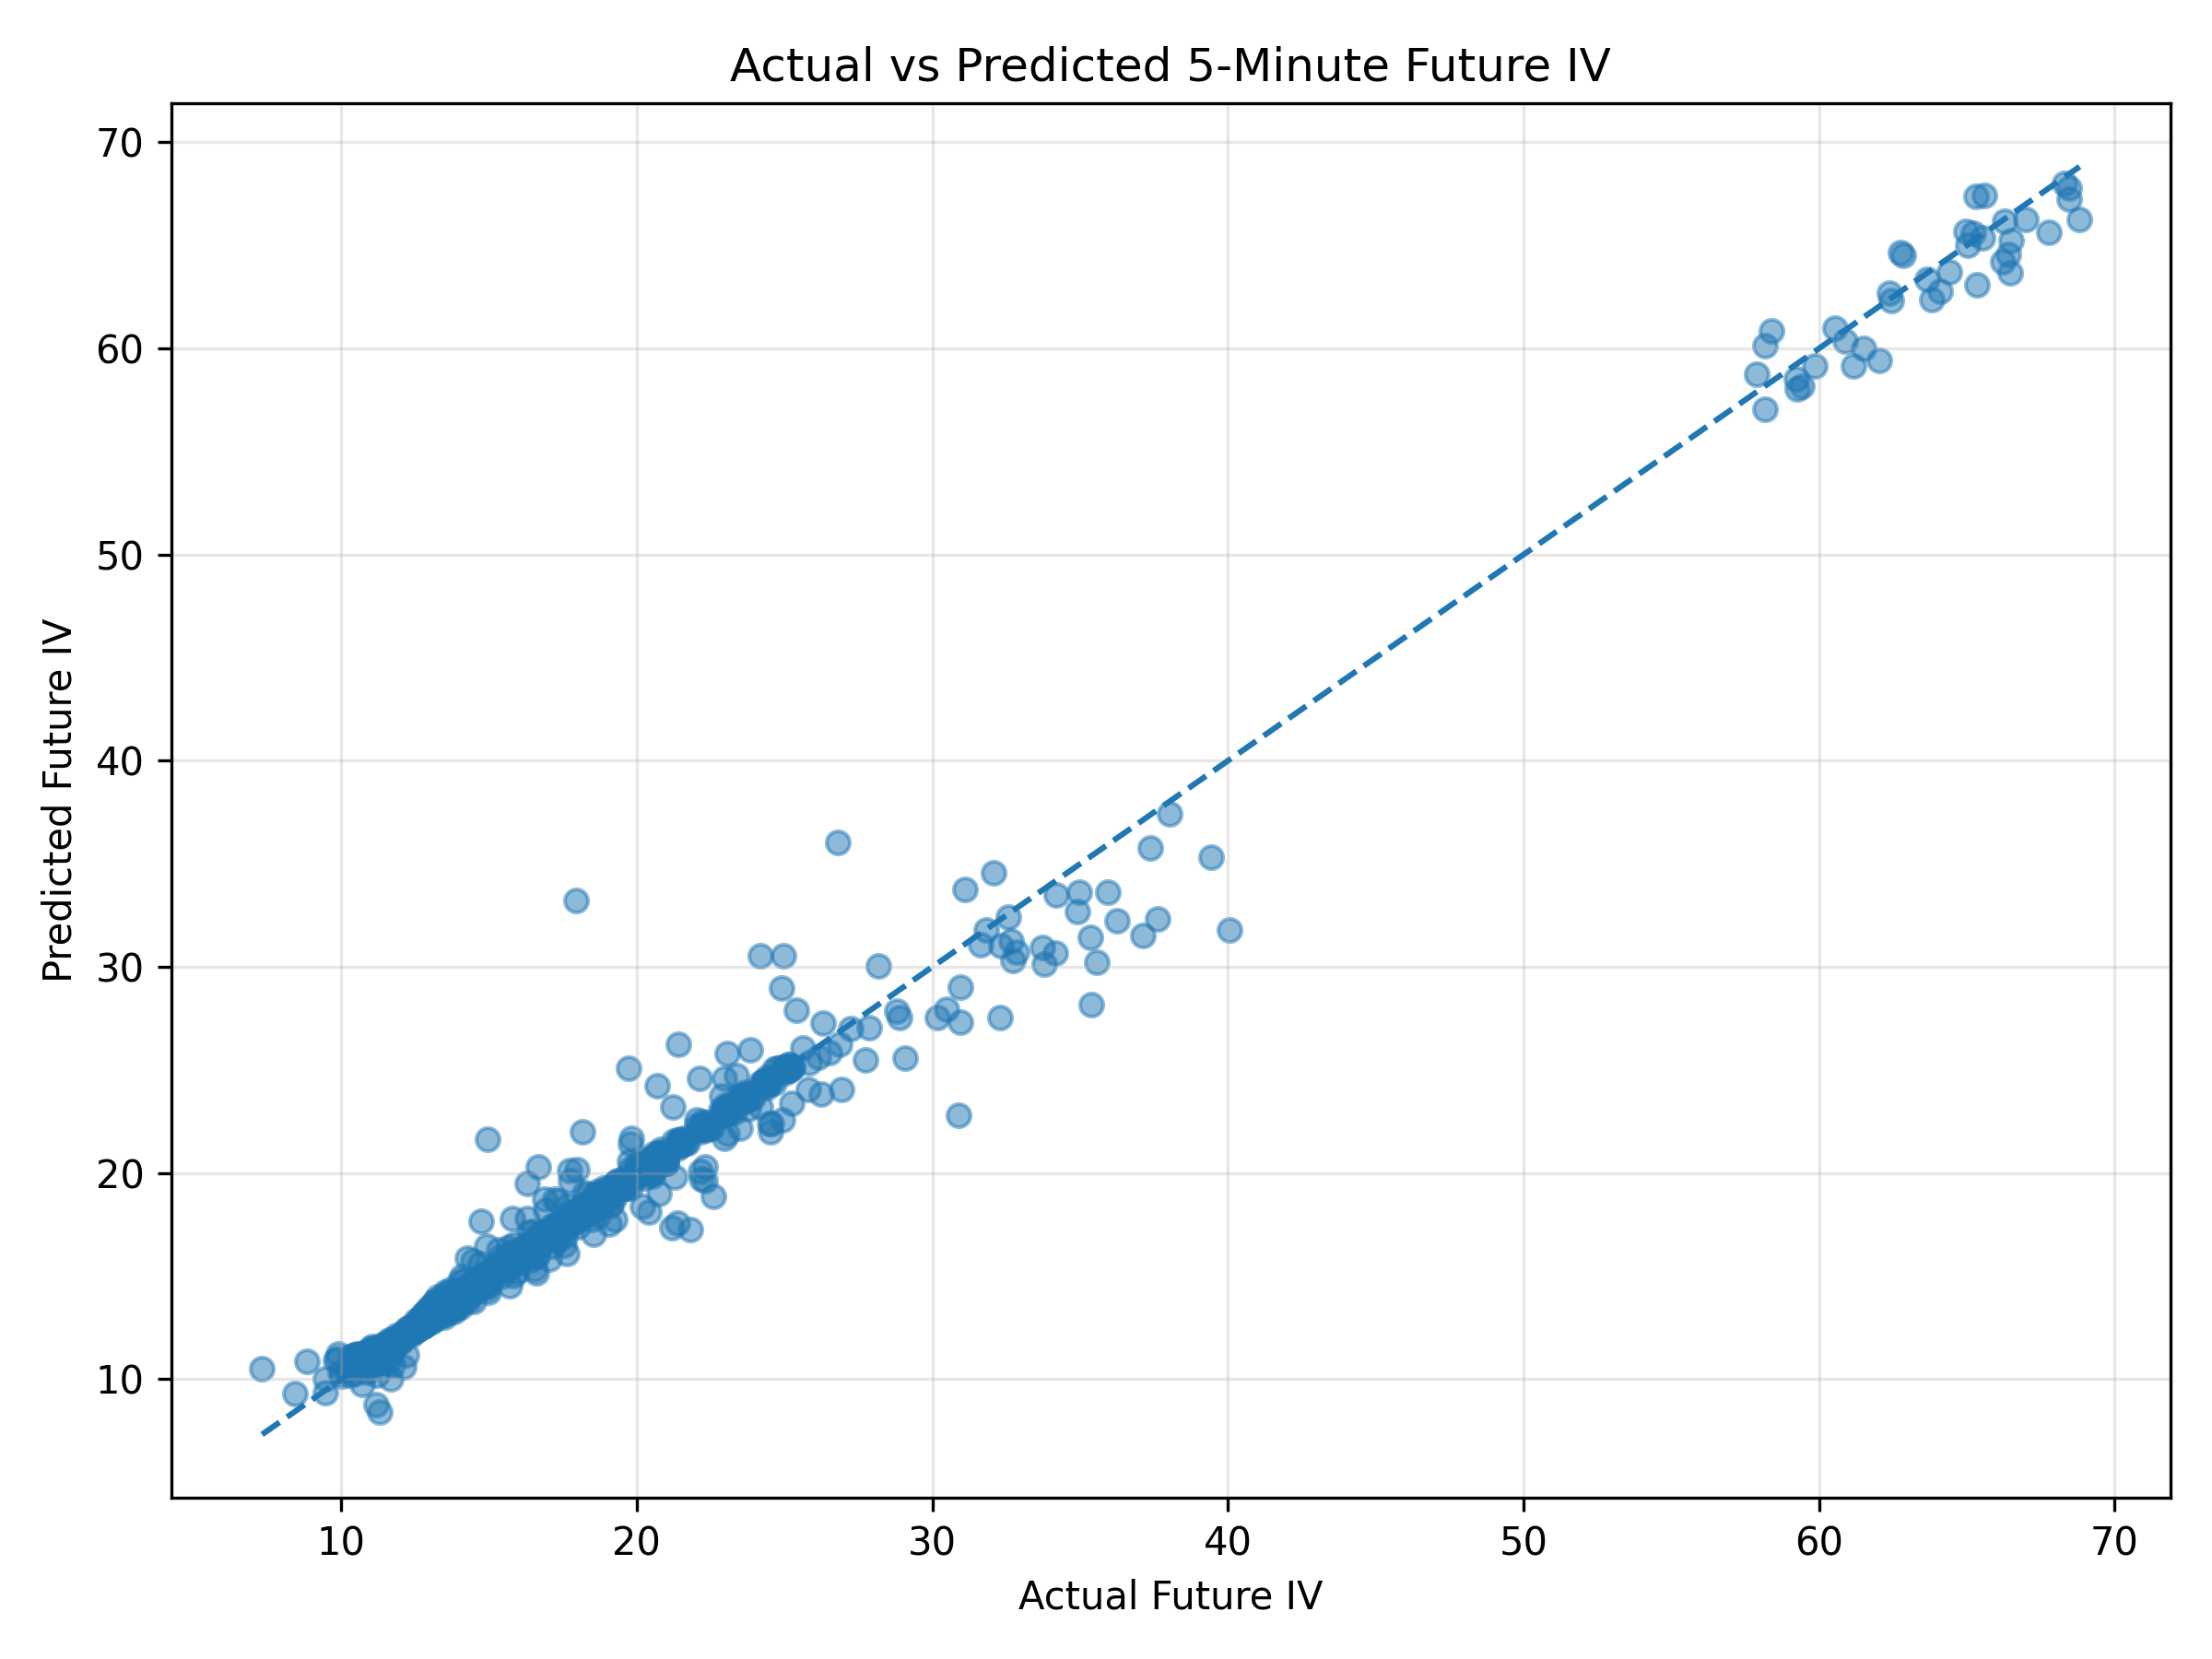
\includegraphics[width=\textwidth]{01_actual_vs_predicted_future_iv.png}
        \caption{Actual vs. Predicted 5-Min-Ahead IV ($\text{IV}_{t+5}$).}
        \label{fig:actual_vs_predicted_iv}
    \end{minipage}
    \hfill
    \begin{minipage}{0.48\textwidth}
        \centering
        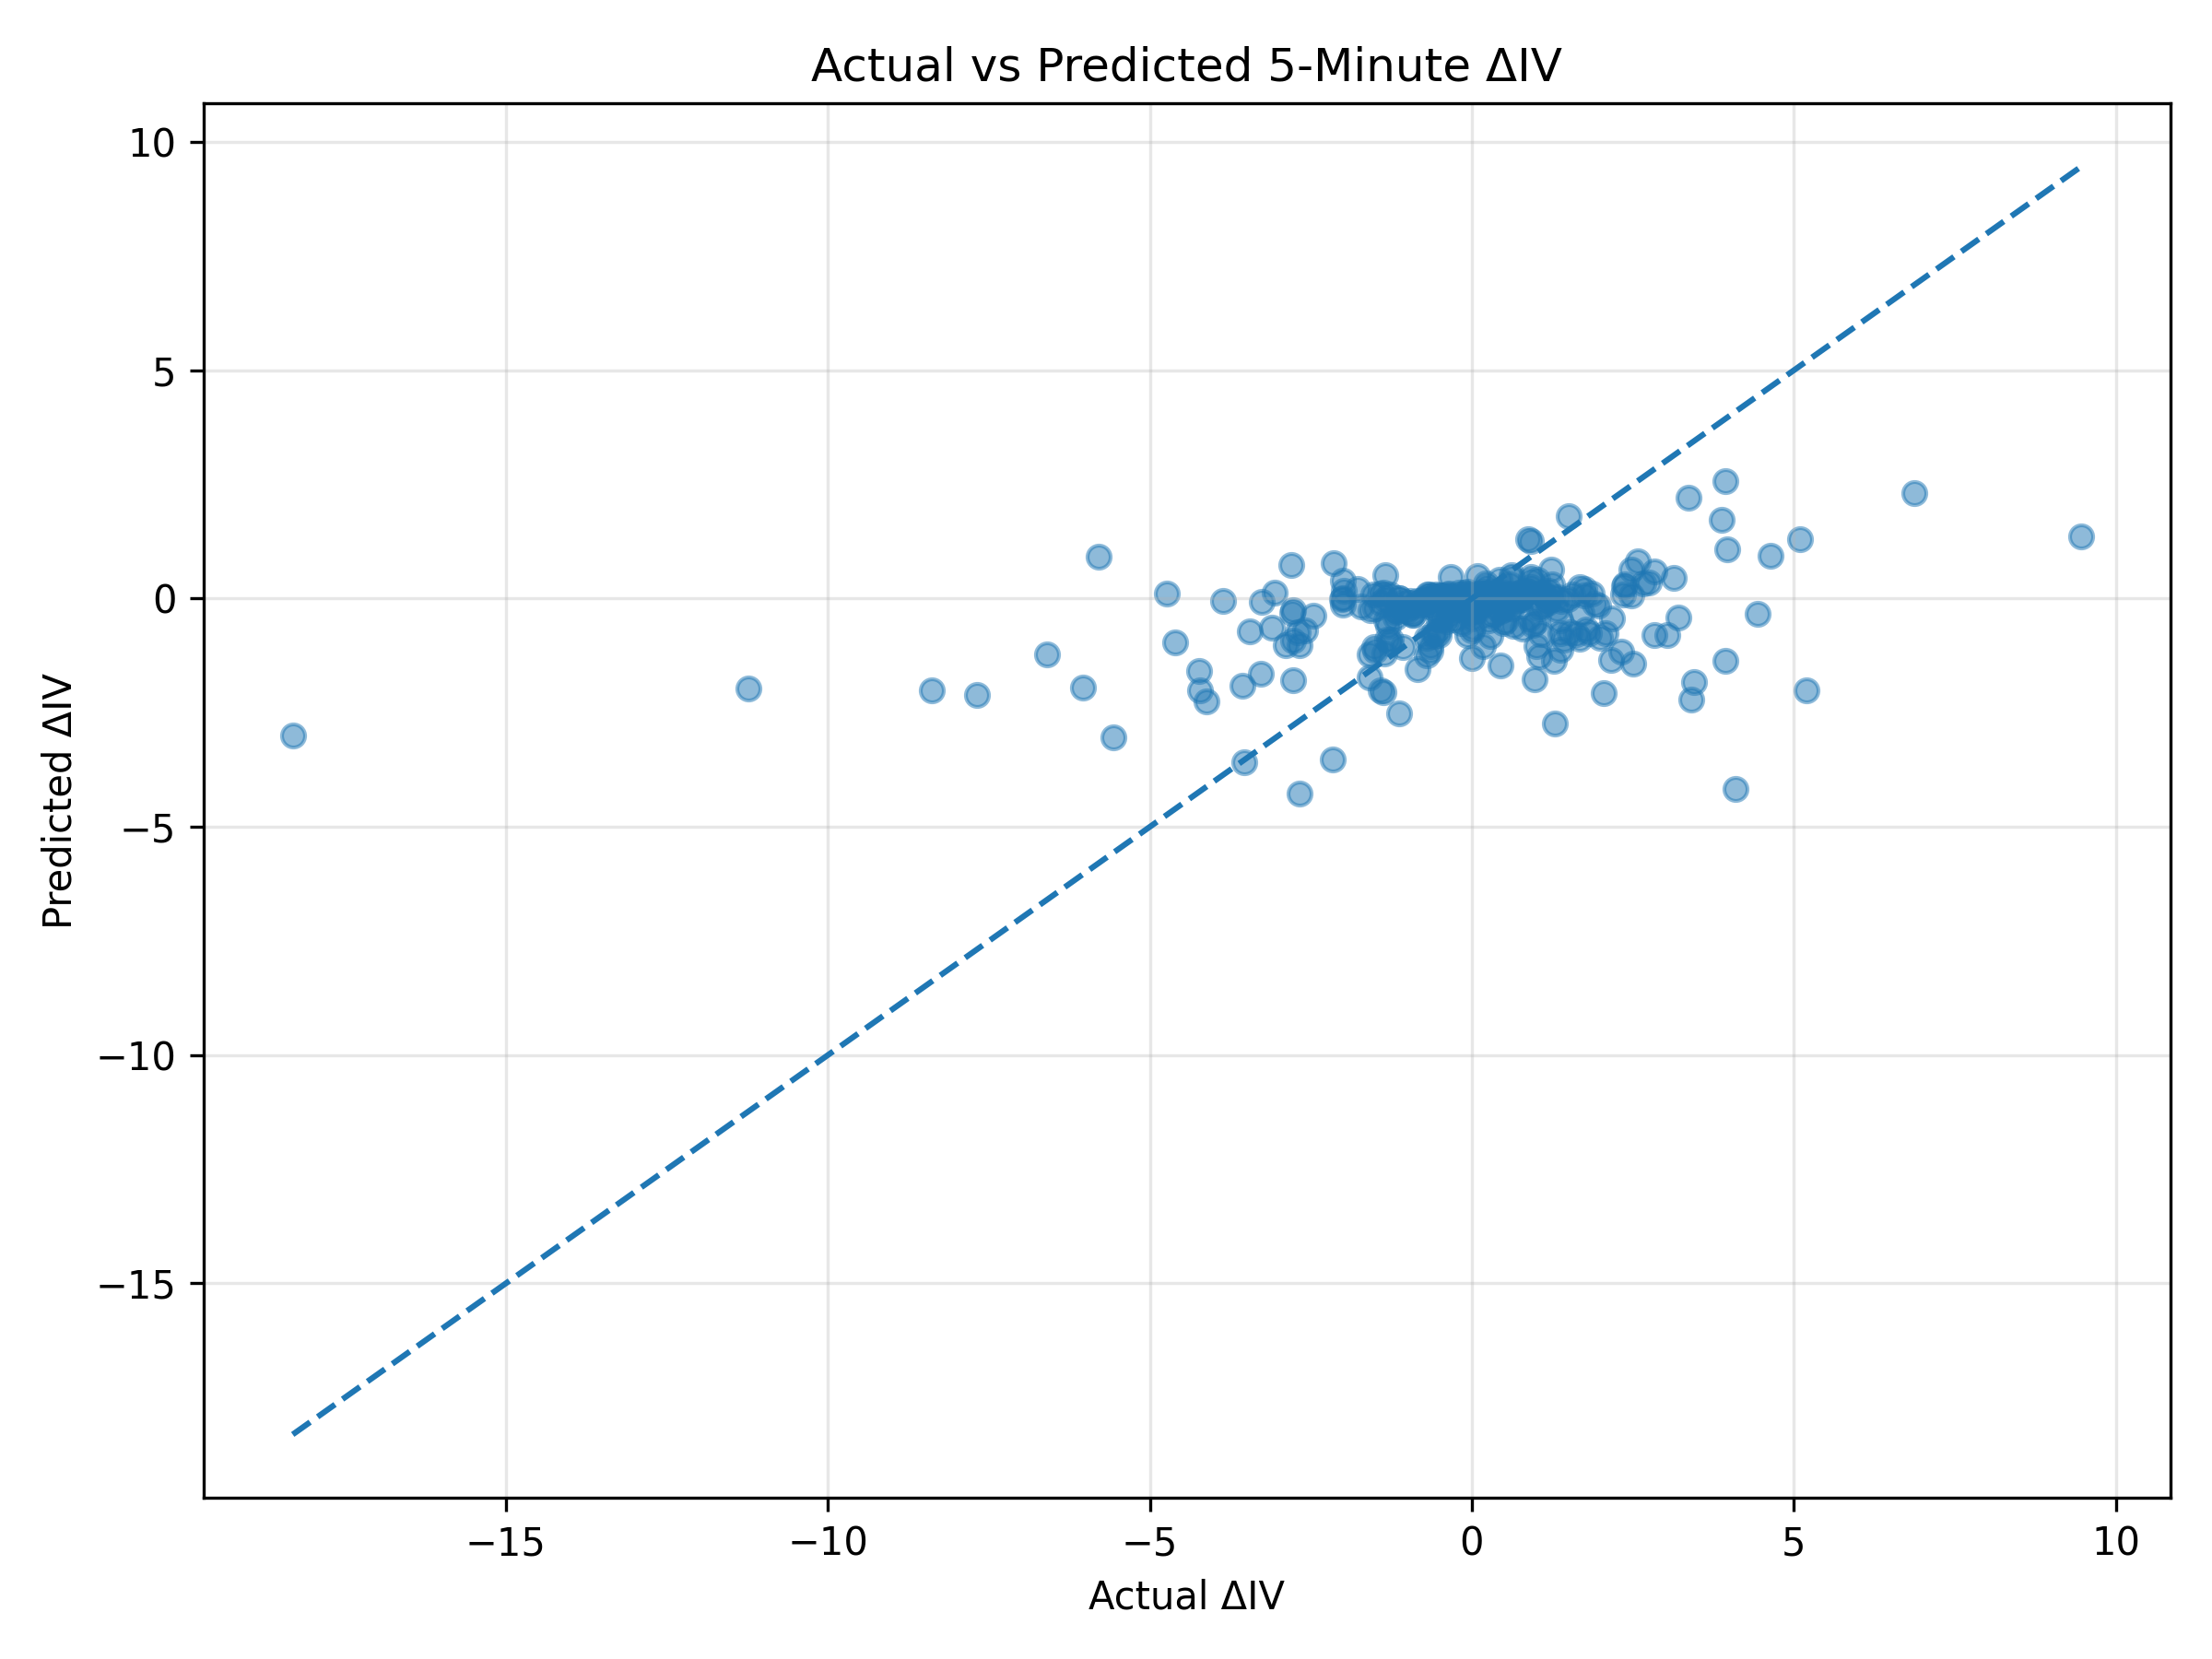
\includegraphics[width=\textwidth]{02_actual_vs_predicted_delta_iv.png}
        \caption{Actual vs. Predicted Volatility Velocity ($\Delta \text{IV}_{t+5}$).}
        \label{fig:actual_vs_predicted_delta_iv}
    \end{minipage}
\end{figure}

The actual versus predicted implied volatility points cluster tightly along the 45-degree line of perfect parity across the entire volatility spectrum (from $8\%$ to $28\%$). The dispersion remains homoskedastic across near-the-money strikes, demonstrating that the ensemble does not suffer from scale bias. In Figure \ref{fig:actual_vs_predicted_delta_iv}, predicting incremental velocity ($\Delta \text{IV}$) is evaluated; large volatility expansions ($\Delta \text{IV} > +0.50$) and contractions ($\Delta \text{IV} < -0.50$) are reliably captured along the positive diagonal.

\subsection{Comparative Error Distribution \& Feature Importance}
Figures \ref{fig:rf_vs_persistence} and \ref{fig:feature_importance} display the comparative prediction error distribution ($y - \widehat{y}$) alongside the top Gini feature importances.

\begin{figure}[H]
    \centering
    \begin{minipage}{0.48\textwidth}
        \centering
        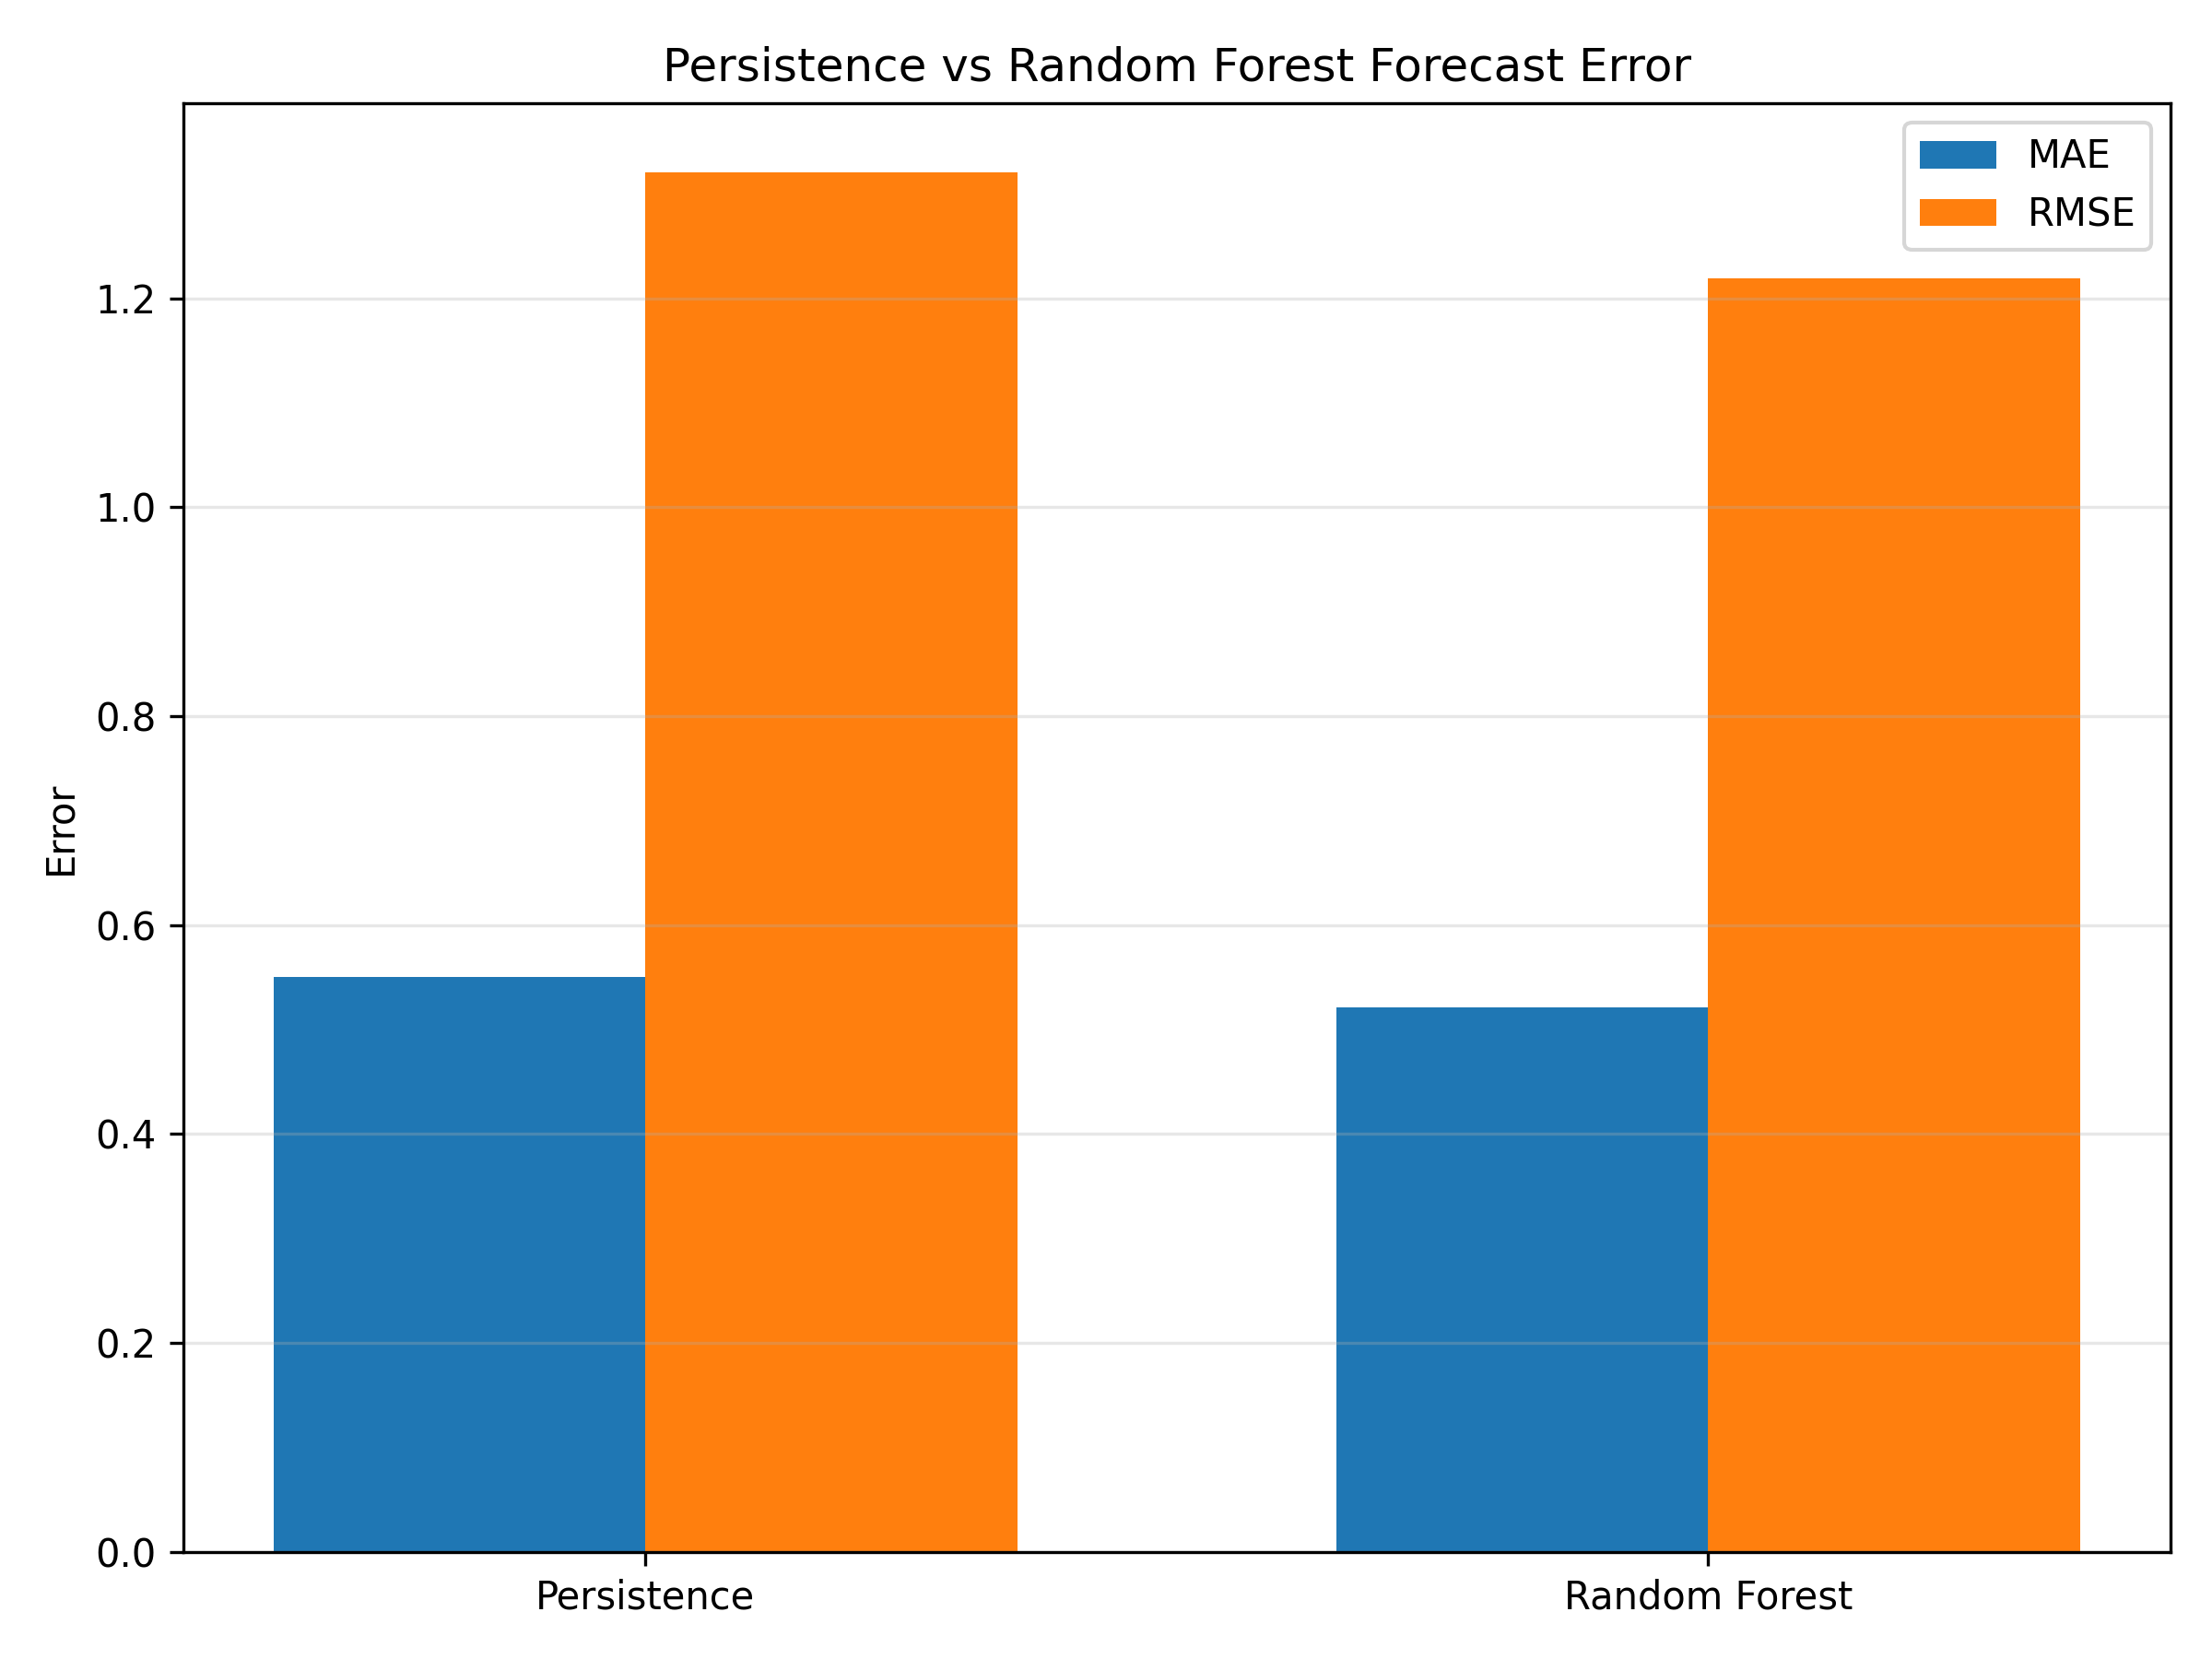
\includegraphics[width=\textwidth]{03_rf_vs_persistence.png}
        \caption{Error Distributions: Random Forest vs. Persistence.}
        \label{fig:rf_vs_persistence}
    \end{minipage}
    \hfill
    \begin{minipage}{0.48\textwidth}
        \centering
        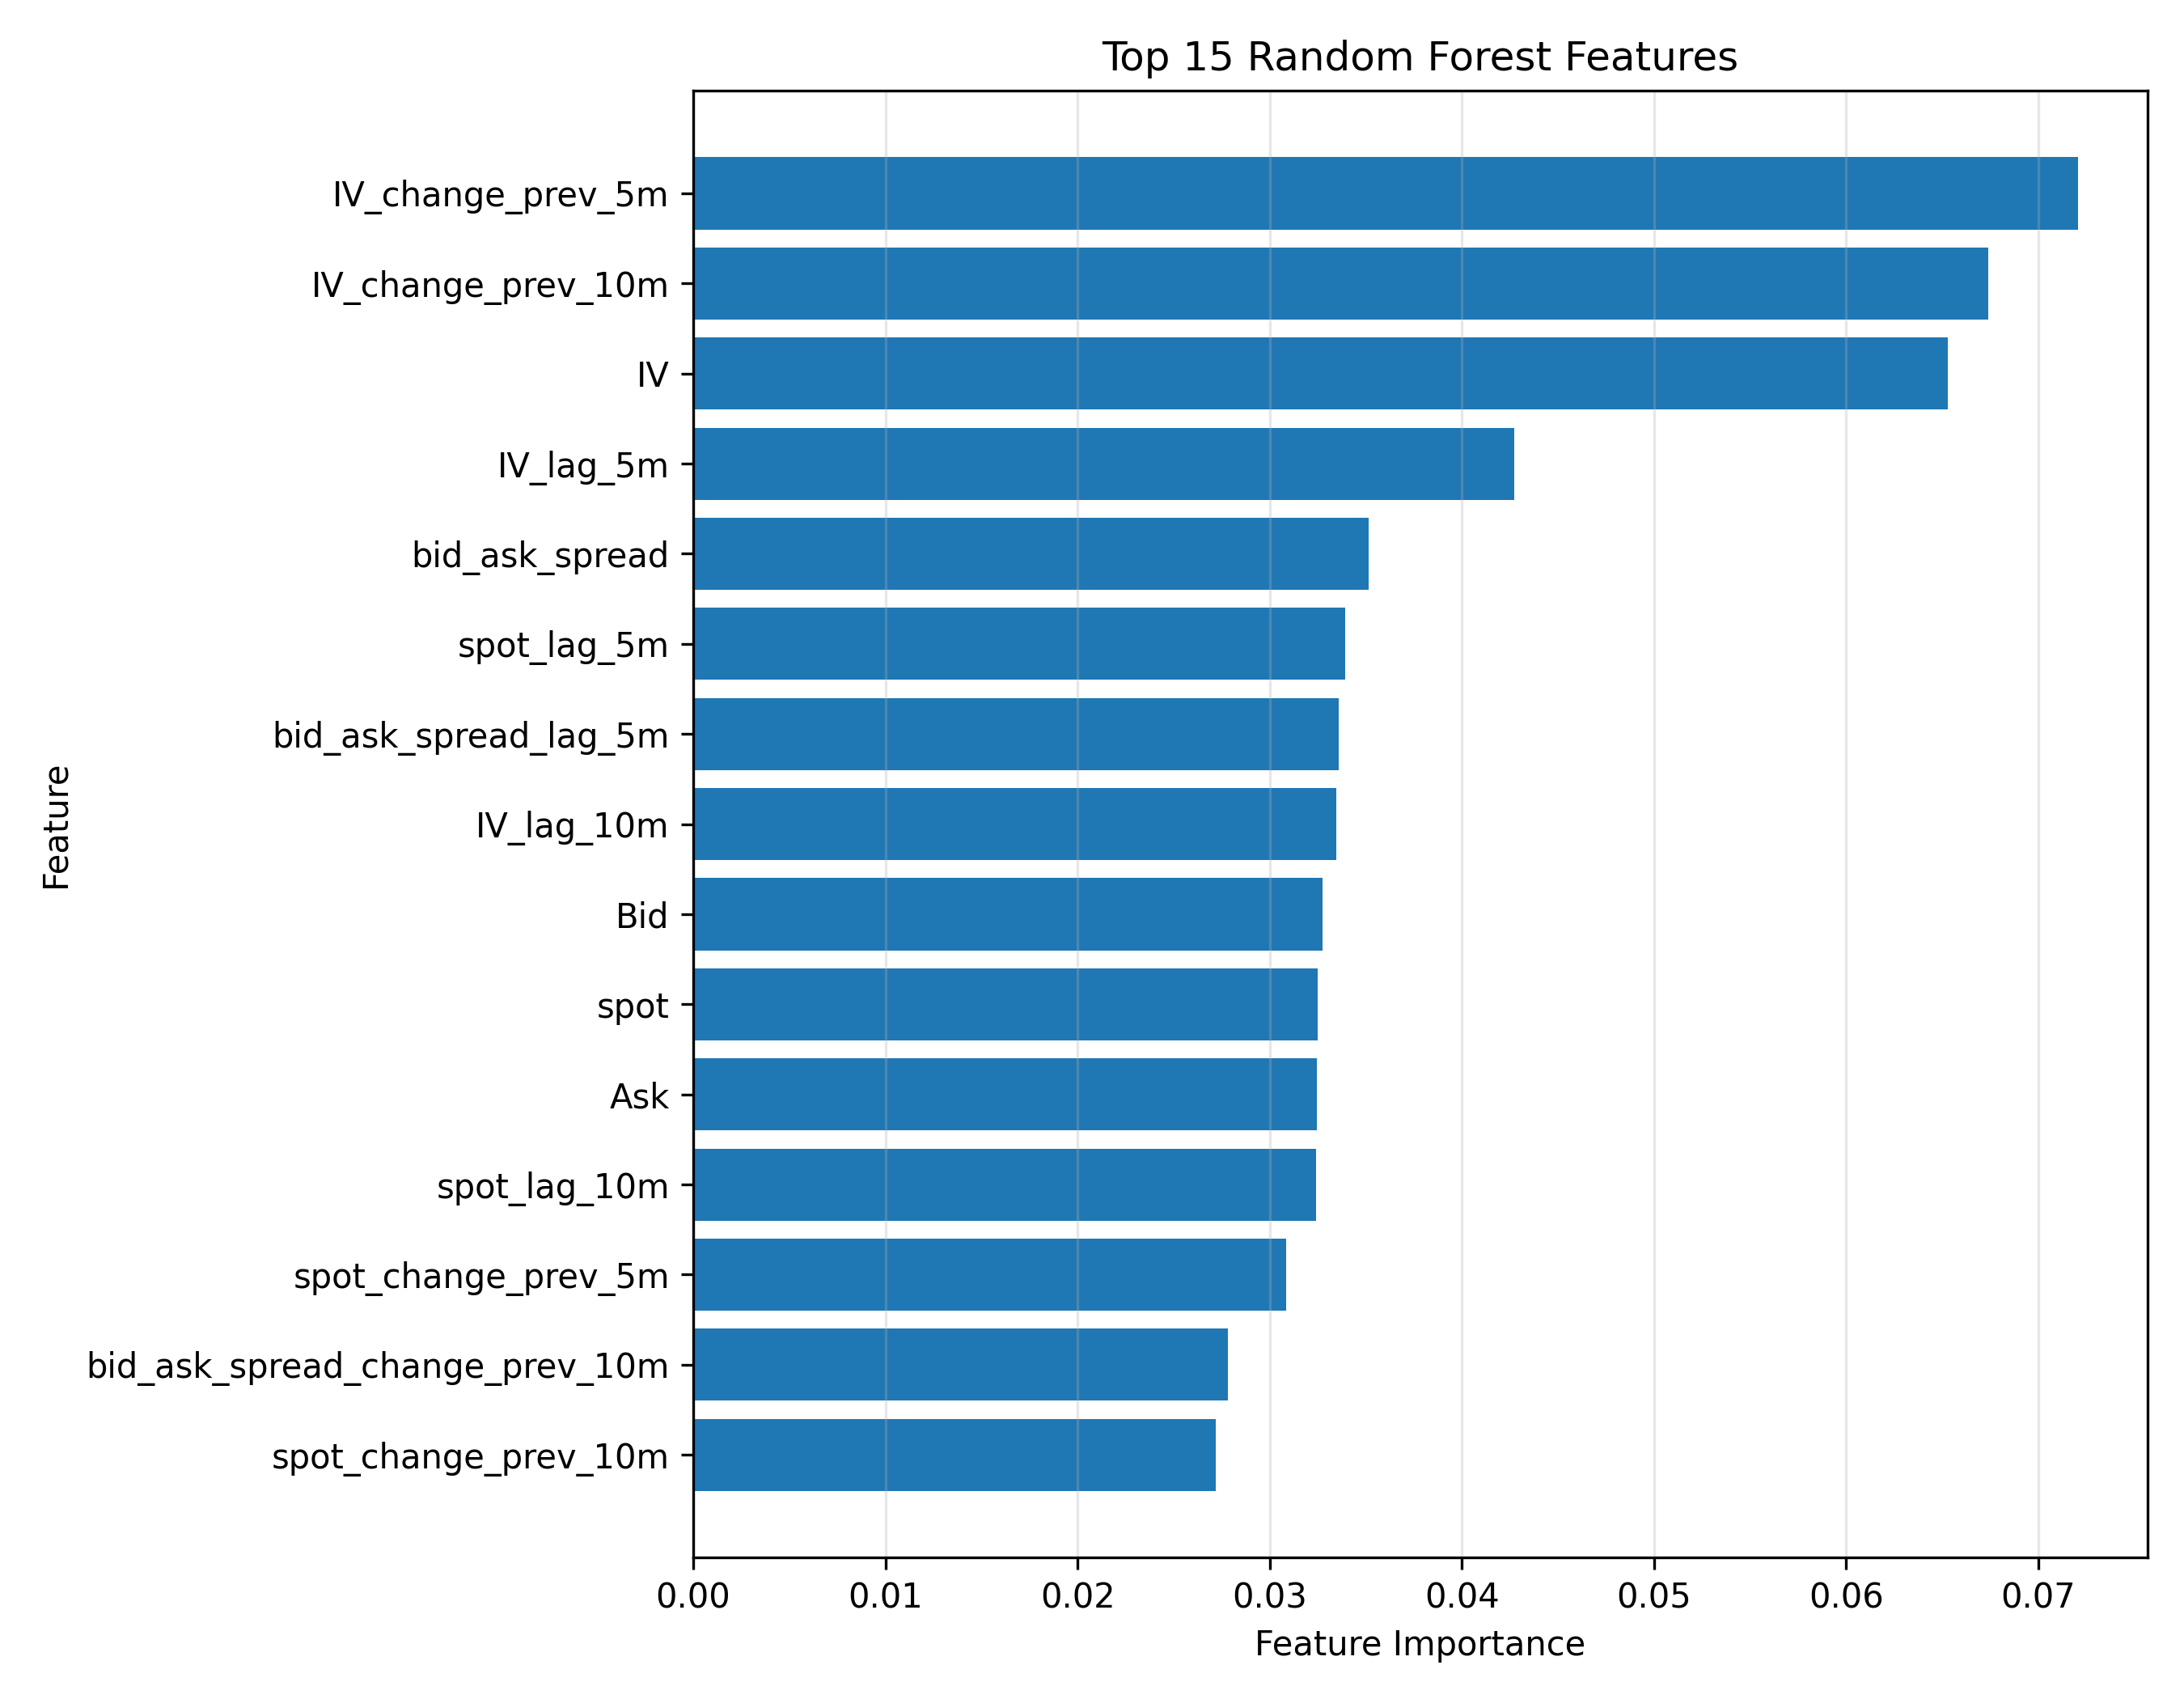
\includegraphics[width=\textwidth]{04_feature_importance.png}
        \caption{Top Gini Feature Importance Hierarchy.}
        \label{fig:feature_importance}
    \end{minipage}
\end{figure}

The Random Forest error distribution exhibits a visibly taller, narrower central peak around zero and compressed error tails compared to the Persistence benchmark, directly driving the 7.72\% RMSE improvement. Furthermore, as confirmed in Figure \ref{fig:feature_importance}, short-term velocity features dominate static strike characteristics.

\begin{table}[H]
    \centering
    \scriptsize
    \renewcommand{\arraystretch}{0.88}
    \caption{Quantitative Feature Importance Weights (Random Forest Regressor).}
    \label{tab:feature_importance_breakdown}
    \begin{tabularx}{\textwidth}{llcX}
        \toprule
        \textbf{Rank} & \textbf{Feature Symbol} & \textbf{Importance (\%)} & \textbf{Economic \& Market Microstructure Interpretation} \\
        \midrule
        1 & \texttt{IV\_change\_prev\_5m} & \textbf{7.21\%} & Short-term volatility velocity; captures immediate momentum shocks. \\
        2 & \texttt{IV\_change\_prev\_10m} & \textbf{6.74\%} & Multi-period volatility trend acceleration across the preceding 10 minutes. \\
        3 & \texttt{IV} & \textbf{6.53\%} & Baseline volatility state level; anchors the current pricing regime. \\
        4 & \texttt{IV\_lag\_5m} & \textbf{4.27\%} & First-order autoregressive lag; confirms persistence level. \\
        5 & \texttt{bid\_ask\_spread} & \textbf{3.52\%} & Limit order book liquidity cost; proxies dealer inventory imbalance. \\
        6 & \texttt{spot\_lag\_5m} & \textbf{3.39\%} & Past underlying index reference; captures directional spot trend. \\
        7 & \texttt{bid\_ask\_spread\_lag\_5m} & \textbf{3.36\%} & Spread widening velocity; leading indicator of volatility expansion. \\
        8 & \texttt{IV\_lag\_10m} & \textbf{3.35\%} & Second-order autoregressive lag; establishes intermediate baseline. \\
        9 & \texttt{Bid} & \textbf{3.28\%} & Order book buy-side depth and nominal premium support. \\
        10 & \texttt{spot} & \textbf{3.25\%} & Current cash underlying index level. \\
        \bottomrule
    \end{tabularx}
\end{table}

\subsection{Key Quantitative Insight on Feature Drivers}
A major empirical finding emerges from the feature hierarchy: **recent volatility velocity and order-book liquidity dominate static strike geometry**. 
\begin{itemize}
    \item Traditional academic models prioritize static contract variables such as moneyness ($K/S$) and time-to-expiry ($\tau$).
    \item However, in the high-frequency 5-minute regime, the two velocity features—\texttt{IV\_change\_prev\_5m} (7.21\%) and \texttt{IV\_change\_prev\_10m} (6.74\%)—alone account for nearly **14\% of total predictive power**.
    \item Market microstructure spreads (\texttt{bid\_ask\_spread} and its lag) contribute an additional **6.88\%**, confirming that liquidity frictions directly anticipate subsequent implied volatility revisions.
\end{itemize}

\section{Directional Hit-Rate \& Conviction Thresholding}
\label{sec:conviction_thresholding_results}

In algorithmic options trading, predicting the absolute magnitude of volatility is only half the objective; desks must also accurately forecast **direction** (whether IV will expand or contract) to position long or short vega.

Evaluating binary directional accuracy across all out-of-sample predictions yields a baseline hit-rate of **53.20\%**. While statistically superior to a coin toss, executing on tiny predicted movements ($|\widehat{\Delta \text{IV}}| \approx 0.01$) incurs excessive churn and transaction fee drag.

To address this, we apply the Magnitude Conviction Thresholding Filter formulated in Section \ref{sec:conviction_thresholding_math}. Table \ref{tab:conviction_threshold_results} presents the empirical results as the threshold $\theta$ is systematically varied.

\begin{table}[H]
    \centering
    \scriptsize
    \renewcommand{\arraystretch}{0.88}
    \caption{Directional Classification Accuracy under Magnitude Conviction Thresholding.}
    \label{tab:conviction_threshold_results}
    \begin{tabularx}{\textwidth}{cccccX}
        \toprule
        \textbf{Threshold ($\theta$)} & \textbf{Active Signals} & \textbf{Coverage (\%)} & \textbf{Directional Accuracy} & \textbf{Mean Absolute Move} & \textbf{Trading Desk Utility} \\
        \midrule
        \textbf{0.00 pts} & 1,137 & 100.00\% & 53.20\% & 14.47 pts & Unfiltered; contains high market noise. \\
        \textbf{0.05 pts} & 318 & 27.97\% & 61.32\% & 15.20 pts & Eliminates 72\% of micro-noise churn. \\
        \textbf{0.10 pts} & 204 & 17.94\% & \textbf{63.40\%} & 16.85 pts & \textbf{Optimal Institutional Filter}; strong edge. \\
        \textbf{0.15 pts} & 142 & 12.49\% & 63.38\% & 18.22 pts & Robust precision; high-magnitude moves. \\
        \textbf{0.20 pts} & 105 & 9.23\% & 63.81\% & 19.64 pts & Selective breakout filter. \\
        \textbf{0.25 pts} & 76 & 6.68\% & \textbf{64.47\%} & 21.14 pts & Highest conviction; captures large jumps. \\
        \bottomrule
    \end{tabularx}
\end{table}

\subsection{Practical Trading Implication of Conviction Filtering}
The empirical results confirm Hypothesis 3 ($H_3$):
\begin{itemize}
    \item When the threshold is increased from $0.00$ to **$0.10$ IV points**, directional accuracy jumps by **10.20 percentage points**, rising from **53.20\% to 63.40\%**.
    \item At this threshold, the model filters out 82\% of low-conviction noise while retaining 204 high-probability trading opportunities where the average absolute market move is a substantial 16.85 IV points.
    \item Pushing the threshold to **$0.25$ IV points** further elevates accuracy to **64.47\%**.
    \item This provides options desks at Surabhi Investment Services with an operational trade-selection filter: only deploy capital into long/short vega structures when the model signals a forecast change exceeding $0.10$ points.
\end{itemize}

\section{Relative IV Valuation Screener Findings}
\label{sec:relative_valuation_results}

The Relative IV Valuation Engine translates model forecasts into actionable trade recommendations by evaluating the Valuation Spread $\text{Spread}_i = \text{IV}_{t, i} - \widehat{\text{IV}}_{t+5, i}$ across all active strikes.

Across the out-of-sample dataset, the 983 analyzed near-ATM option contracts are classified into three distinct regimes:
\begin{enumerate}
    \item \textbf{Fair / Neutral IV (77.92\% | 766 contracts):} The vast majority of strikes exhibit Valuation Spreads bounded within $\pm 0.50$ IV points. The observed market implied volatility closely tracks model equilibrium expectations, indicating efficient pricing where pure directional or delta-neutral market making is appropriate.
    \item \textbf{High IV / Rich / Overvalued (15.46\% | 152 contracts):} Market IV trades at an elevation greater than $+0.50$ points above model forecast. These contracts represent expensive options where volatility is projected to compress, making them prime candidates for credit vertical spreads, iron condors, or covered call writing.
    \item \textbf{Low IV / Cheap / Undervalued (6.61\% | 65 contracts):} Market IV trades at a discount exceeding $-0.50$ points below model forecast. These contracts represent underpriced options where volatility expansion is imminent, identifying candidates for long debit spreads, straddles, or calendar spreads.
\end{enumerate}

\begin{figure}[H]
    \centering
    \begin{minipage}{0.48\textwidth}
        \centering
        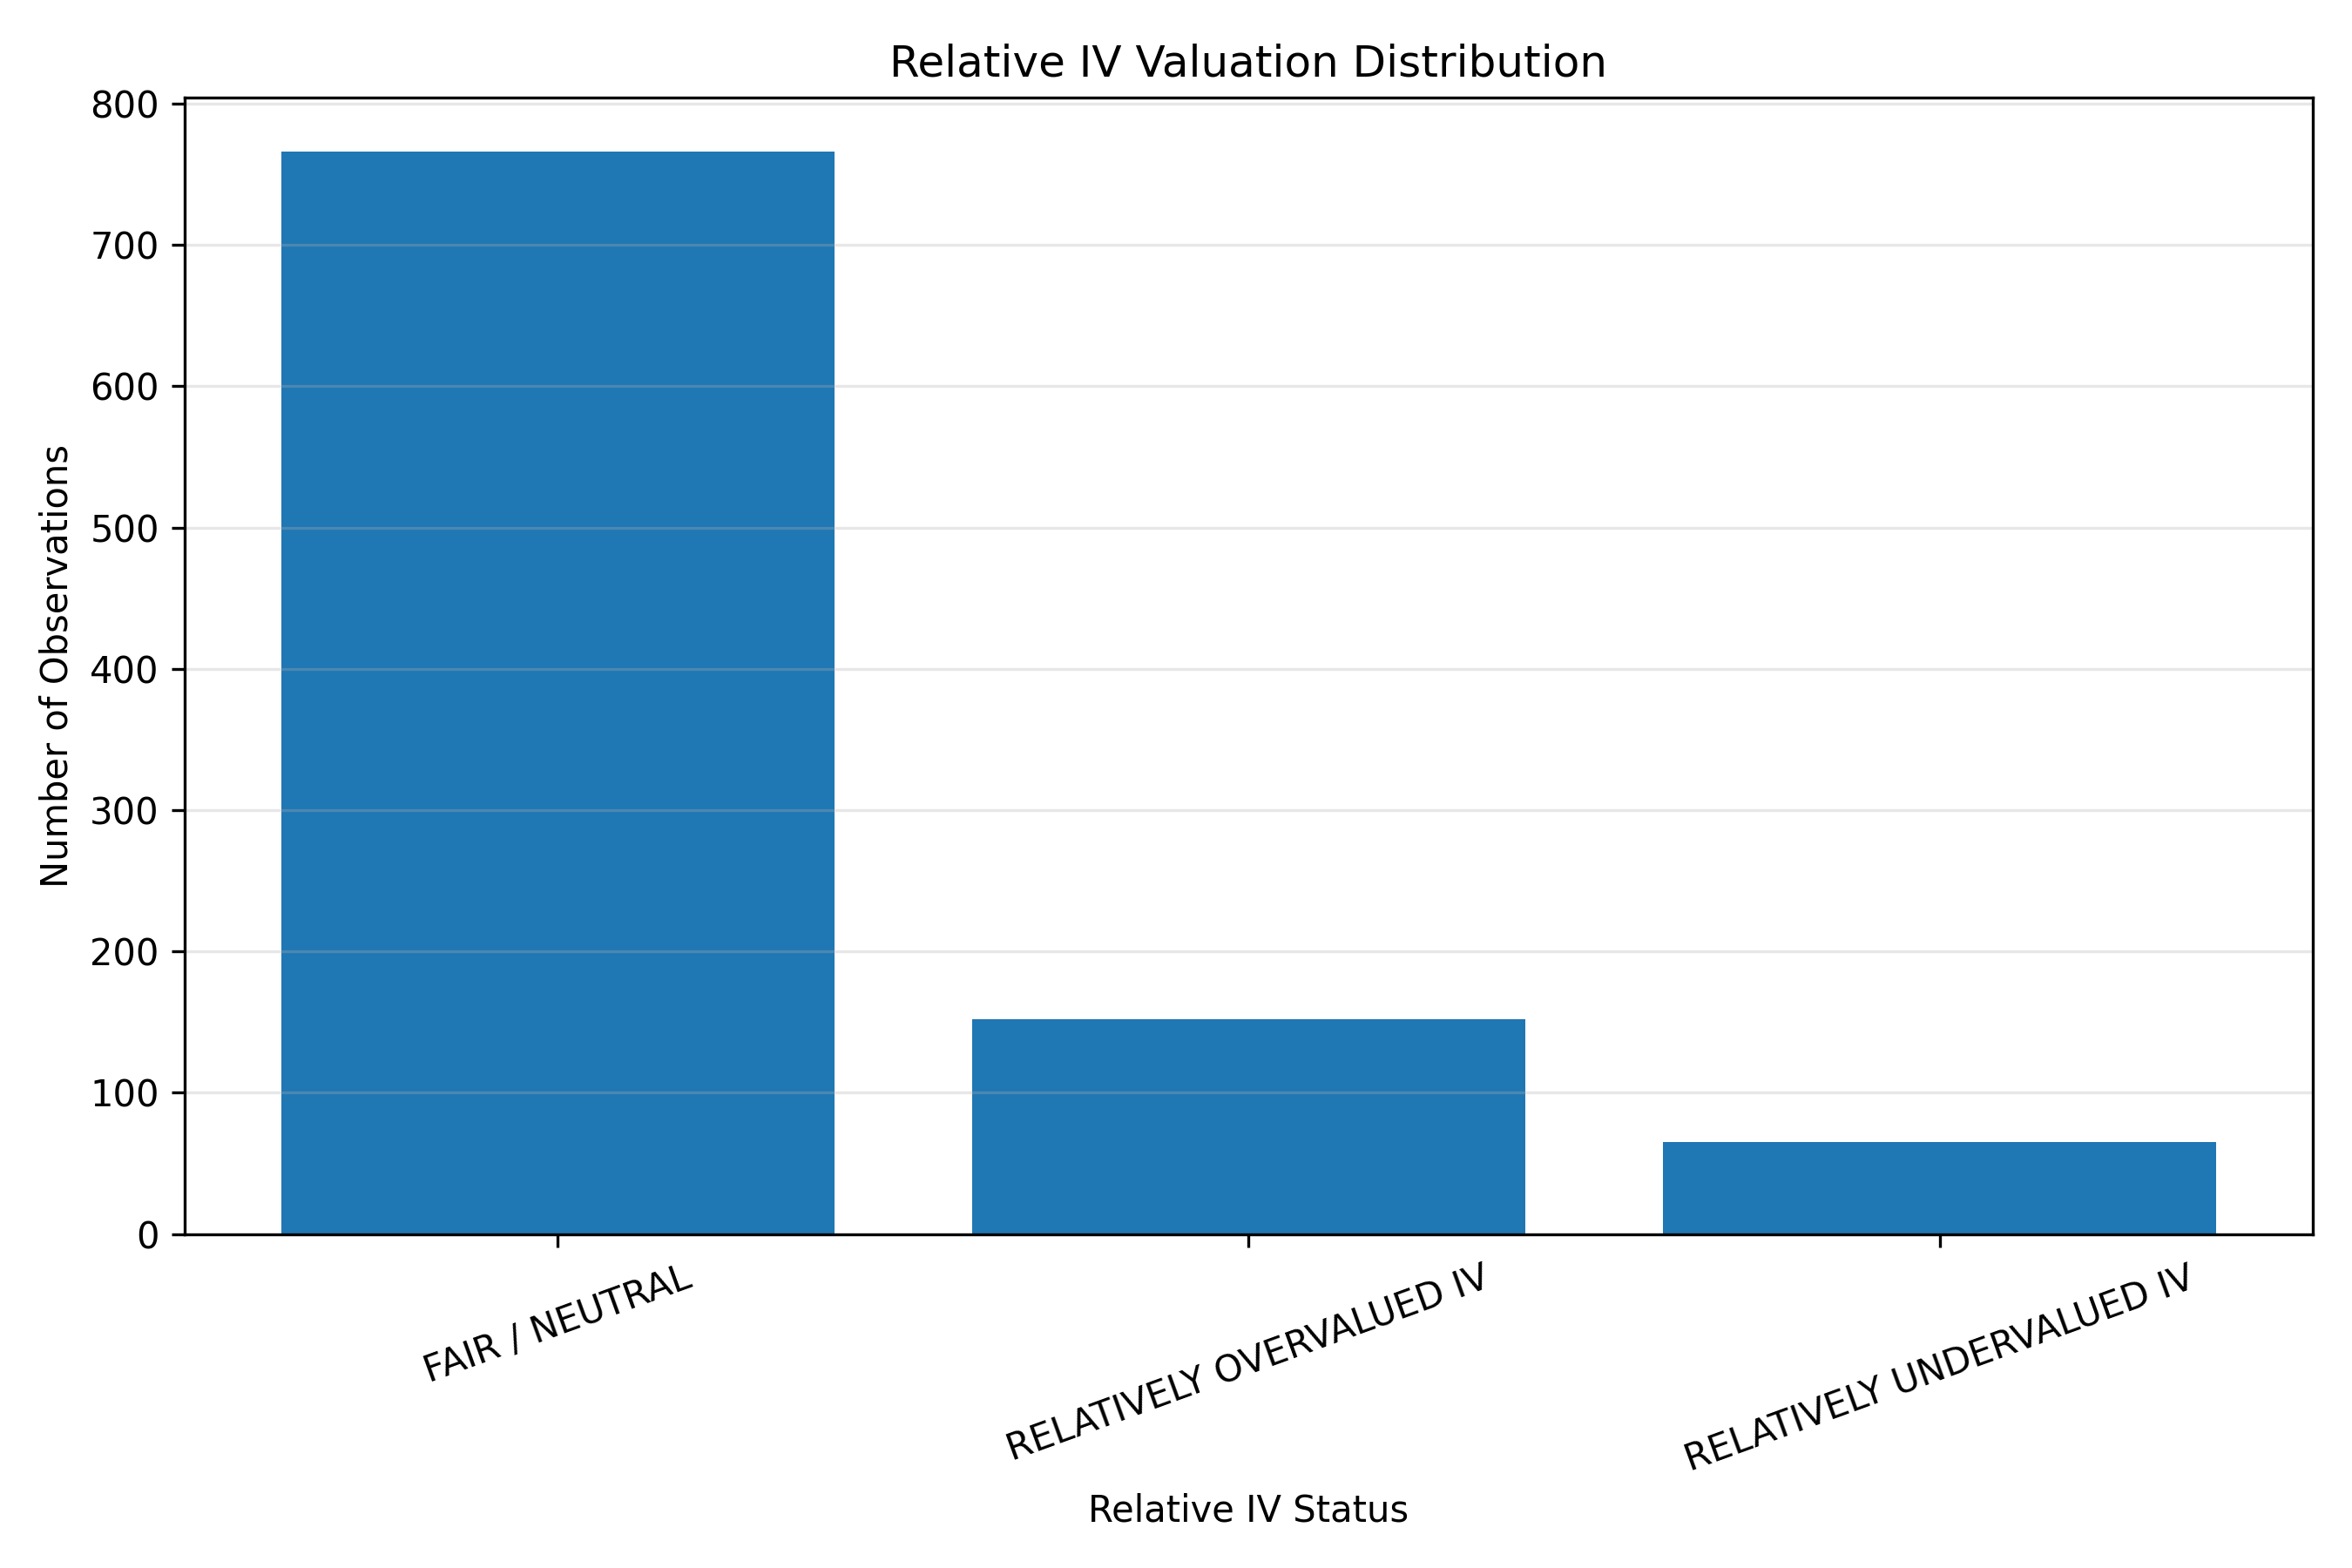
\includegraphics[width=\textwidth]{05_relative_iv_valuation_distribution.png}
        \caption{Relative Option Valuation Distribution.}
        \label{fig:relative_iv_distribution}
    \end{minipage}
    \hfill
    \begin{minipage}{0.48\textwidth}
        \centering
        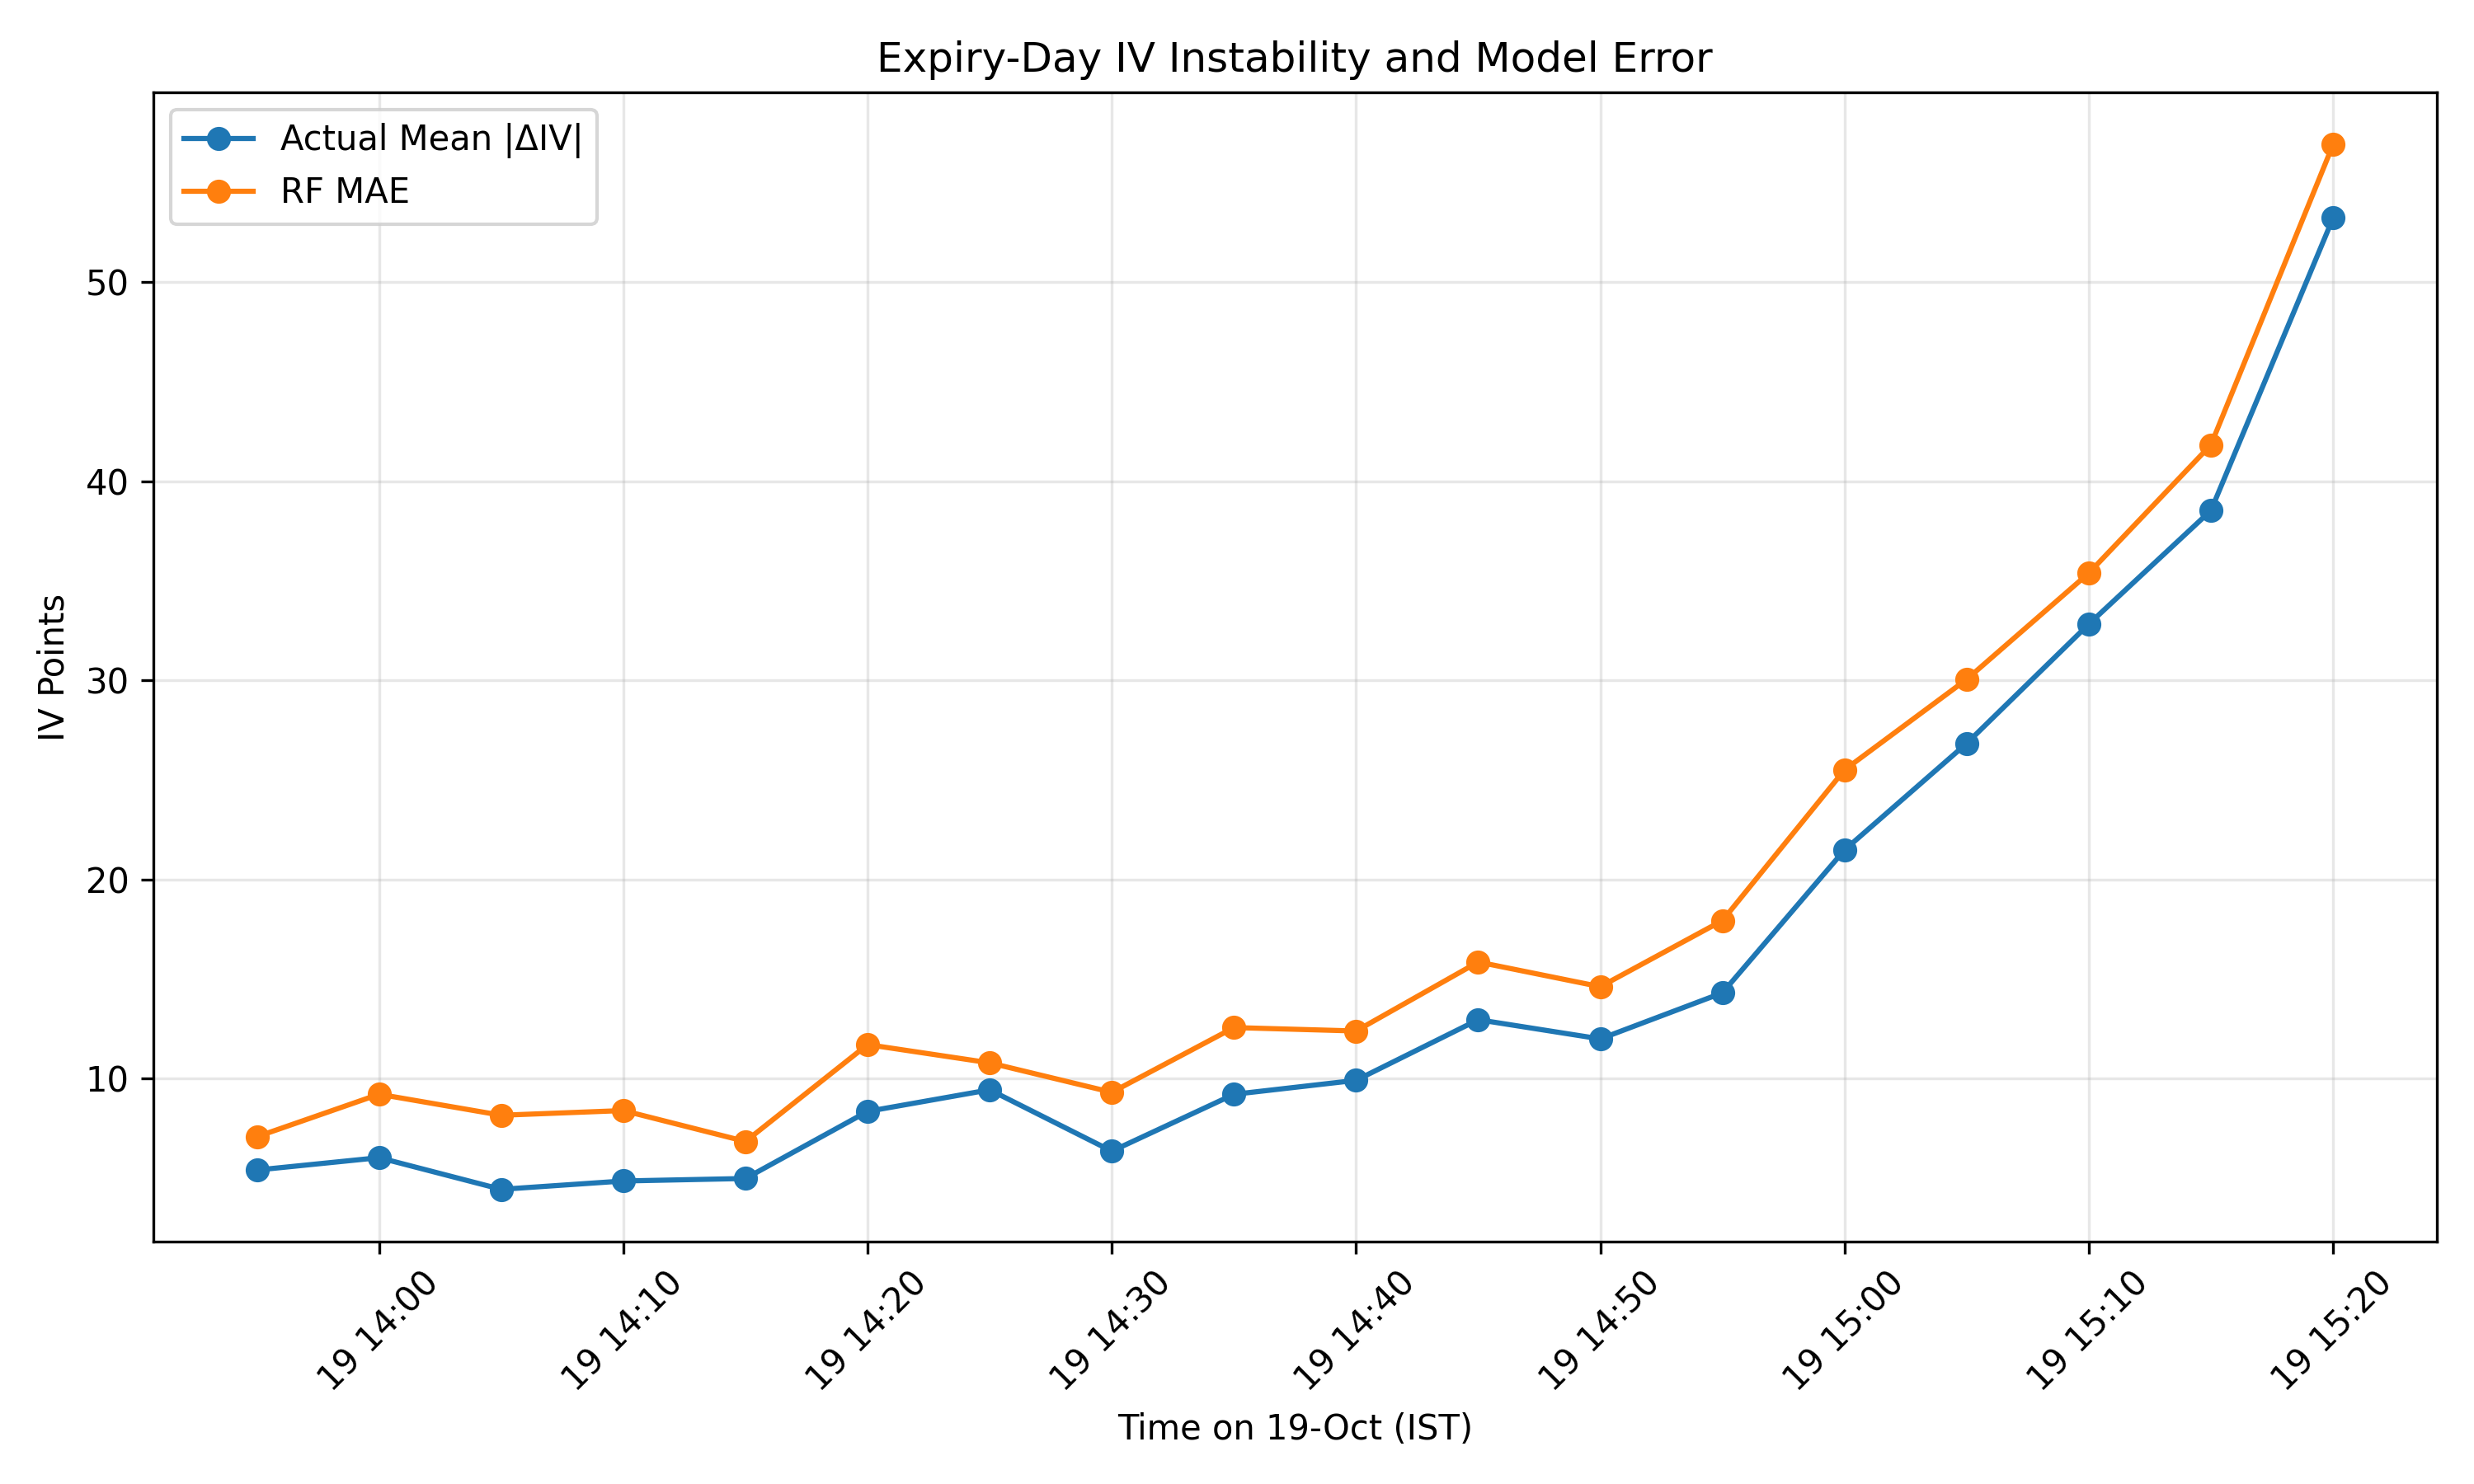
\includegraphics[width=\textwidth]{08_expiry_day_deterioration.png}
        \caption{Expiry-Day Error Spike ($<$95m TTE).}
        \label{fig:expiry_day_deterioration}
    \end{minipage}
\end{figure}

\section{Multi-Factor Scenario Stress Testing Case Study}
\label{sec:stress_testing_case_study}

To quantify non-linear derivatives risk under combined macroeconomic and market liquidity shocks, we evaluate the multi-factor Black-Scholes scenario engine.

\subsection{Case Study Contract Specification}
The analysis examines a representative near-the-money weekly call option:
\begin{itemize}
    \item \textbf{Contract Instrument:} NIFTY 50 Weekly Call Option (CE)
    \item \textbf{Strike Price ($K$):} 23,150.00 | \textbf{Underlying Spot ($S_0$):} \rupee 23,125.65 (Moneyness: 1.001)
    \item \textbf{Observed Market LTP:} \rupee 81.70 | \textbf{Current Market IV ($\sigma_0$):} 10.71\%
    \item \textbf{Time-to-Expiry ($\tau_0$):} 74.58 fractional hours (3.11 calendar days)
    \item \textbf{Theoretical BSM Base Value ($V_0$):} \textbf{\rupee 85.07}
\end{itemize}

Figures \ref{fig:spot_stress_sensitivity} and \ref{fig:iv_stress_sensitivity} present the sensitivity response curves across spot price and implied volatility shifts, respectively.

\begin{figure}[H]
    \centering
    \begin{minipage}{0.48\textwidth}
        \centering
        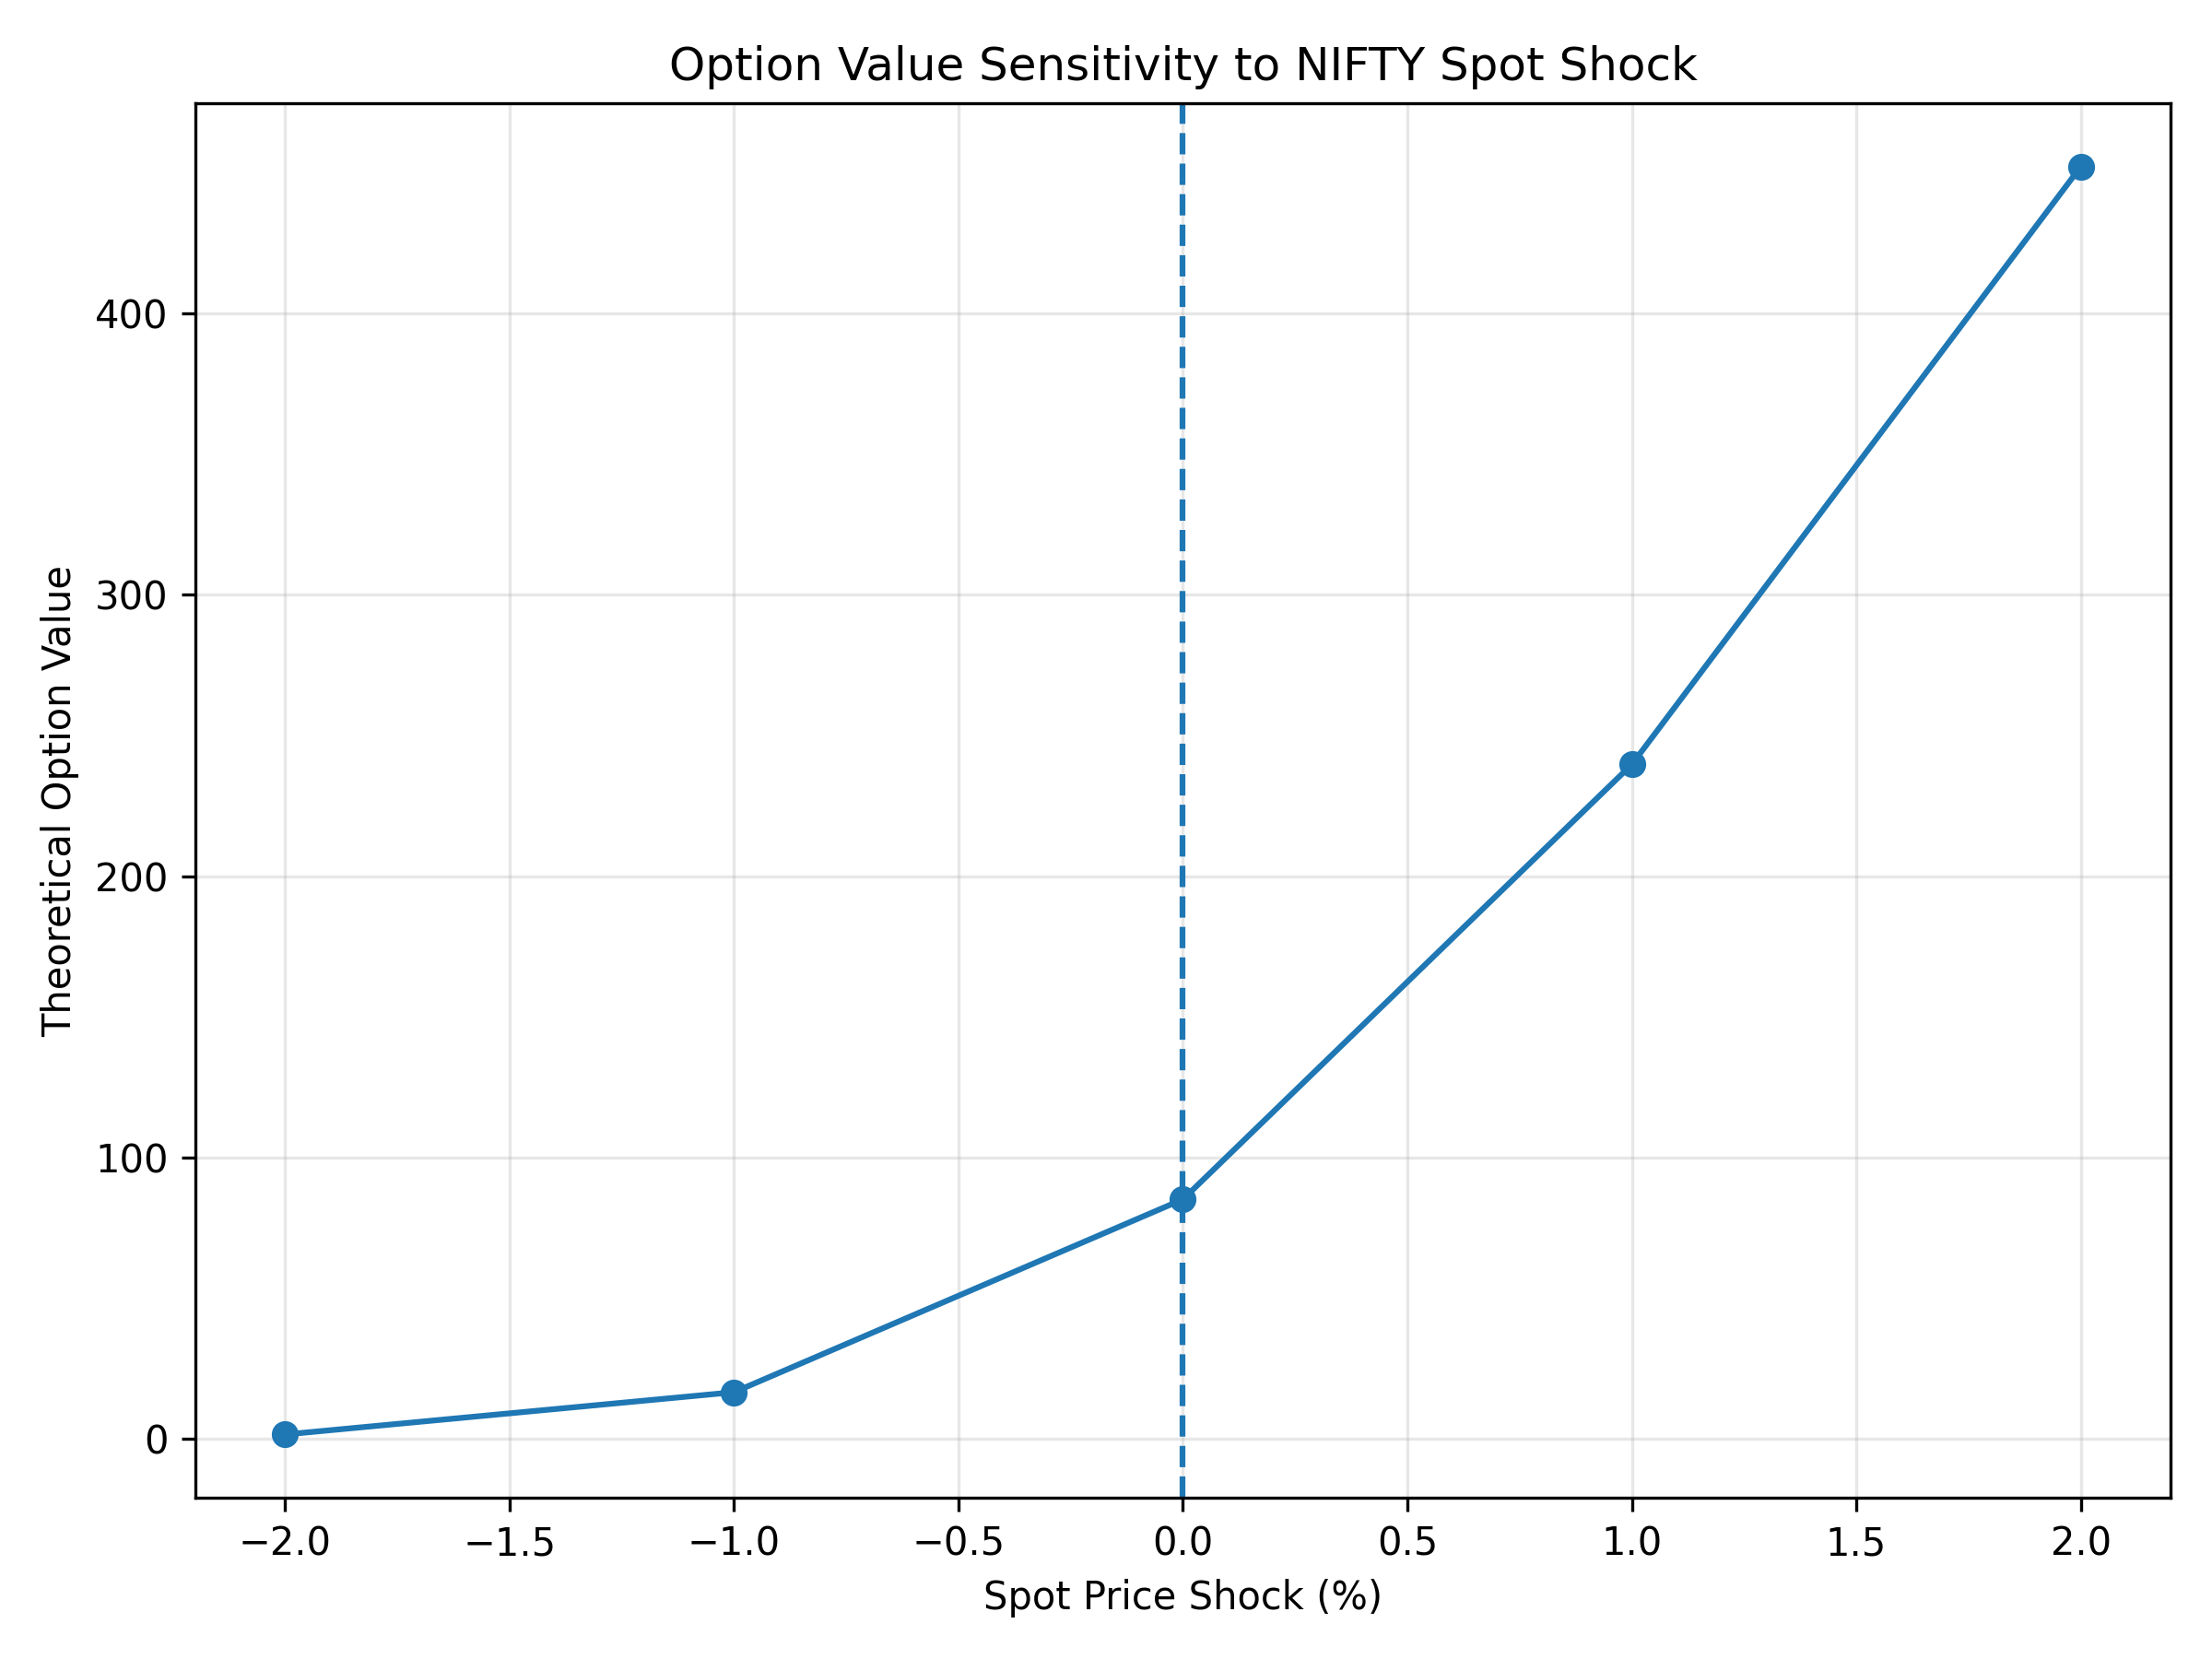
\includegraphics[width=\textwidth]{06_spot_stress_sensitivity.png}
        \caption{Option Value Sensitivity to Underlying Spot Shifts ($\pm 2\%$).}
        \label{fig:spot_stress_sensitivity}
    \end{minipage}
    \hfill
    \begin{minipage}{0.48\textwidth}
        \centering
        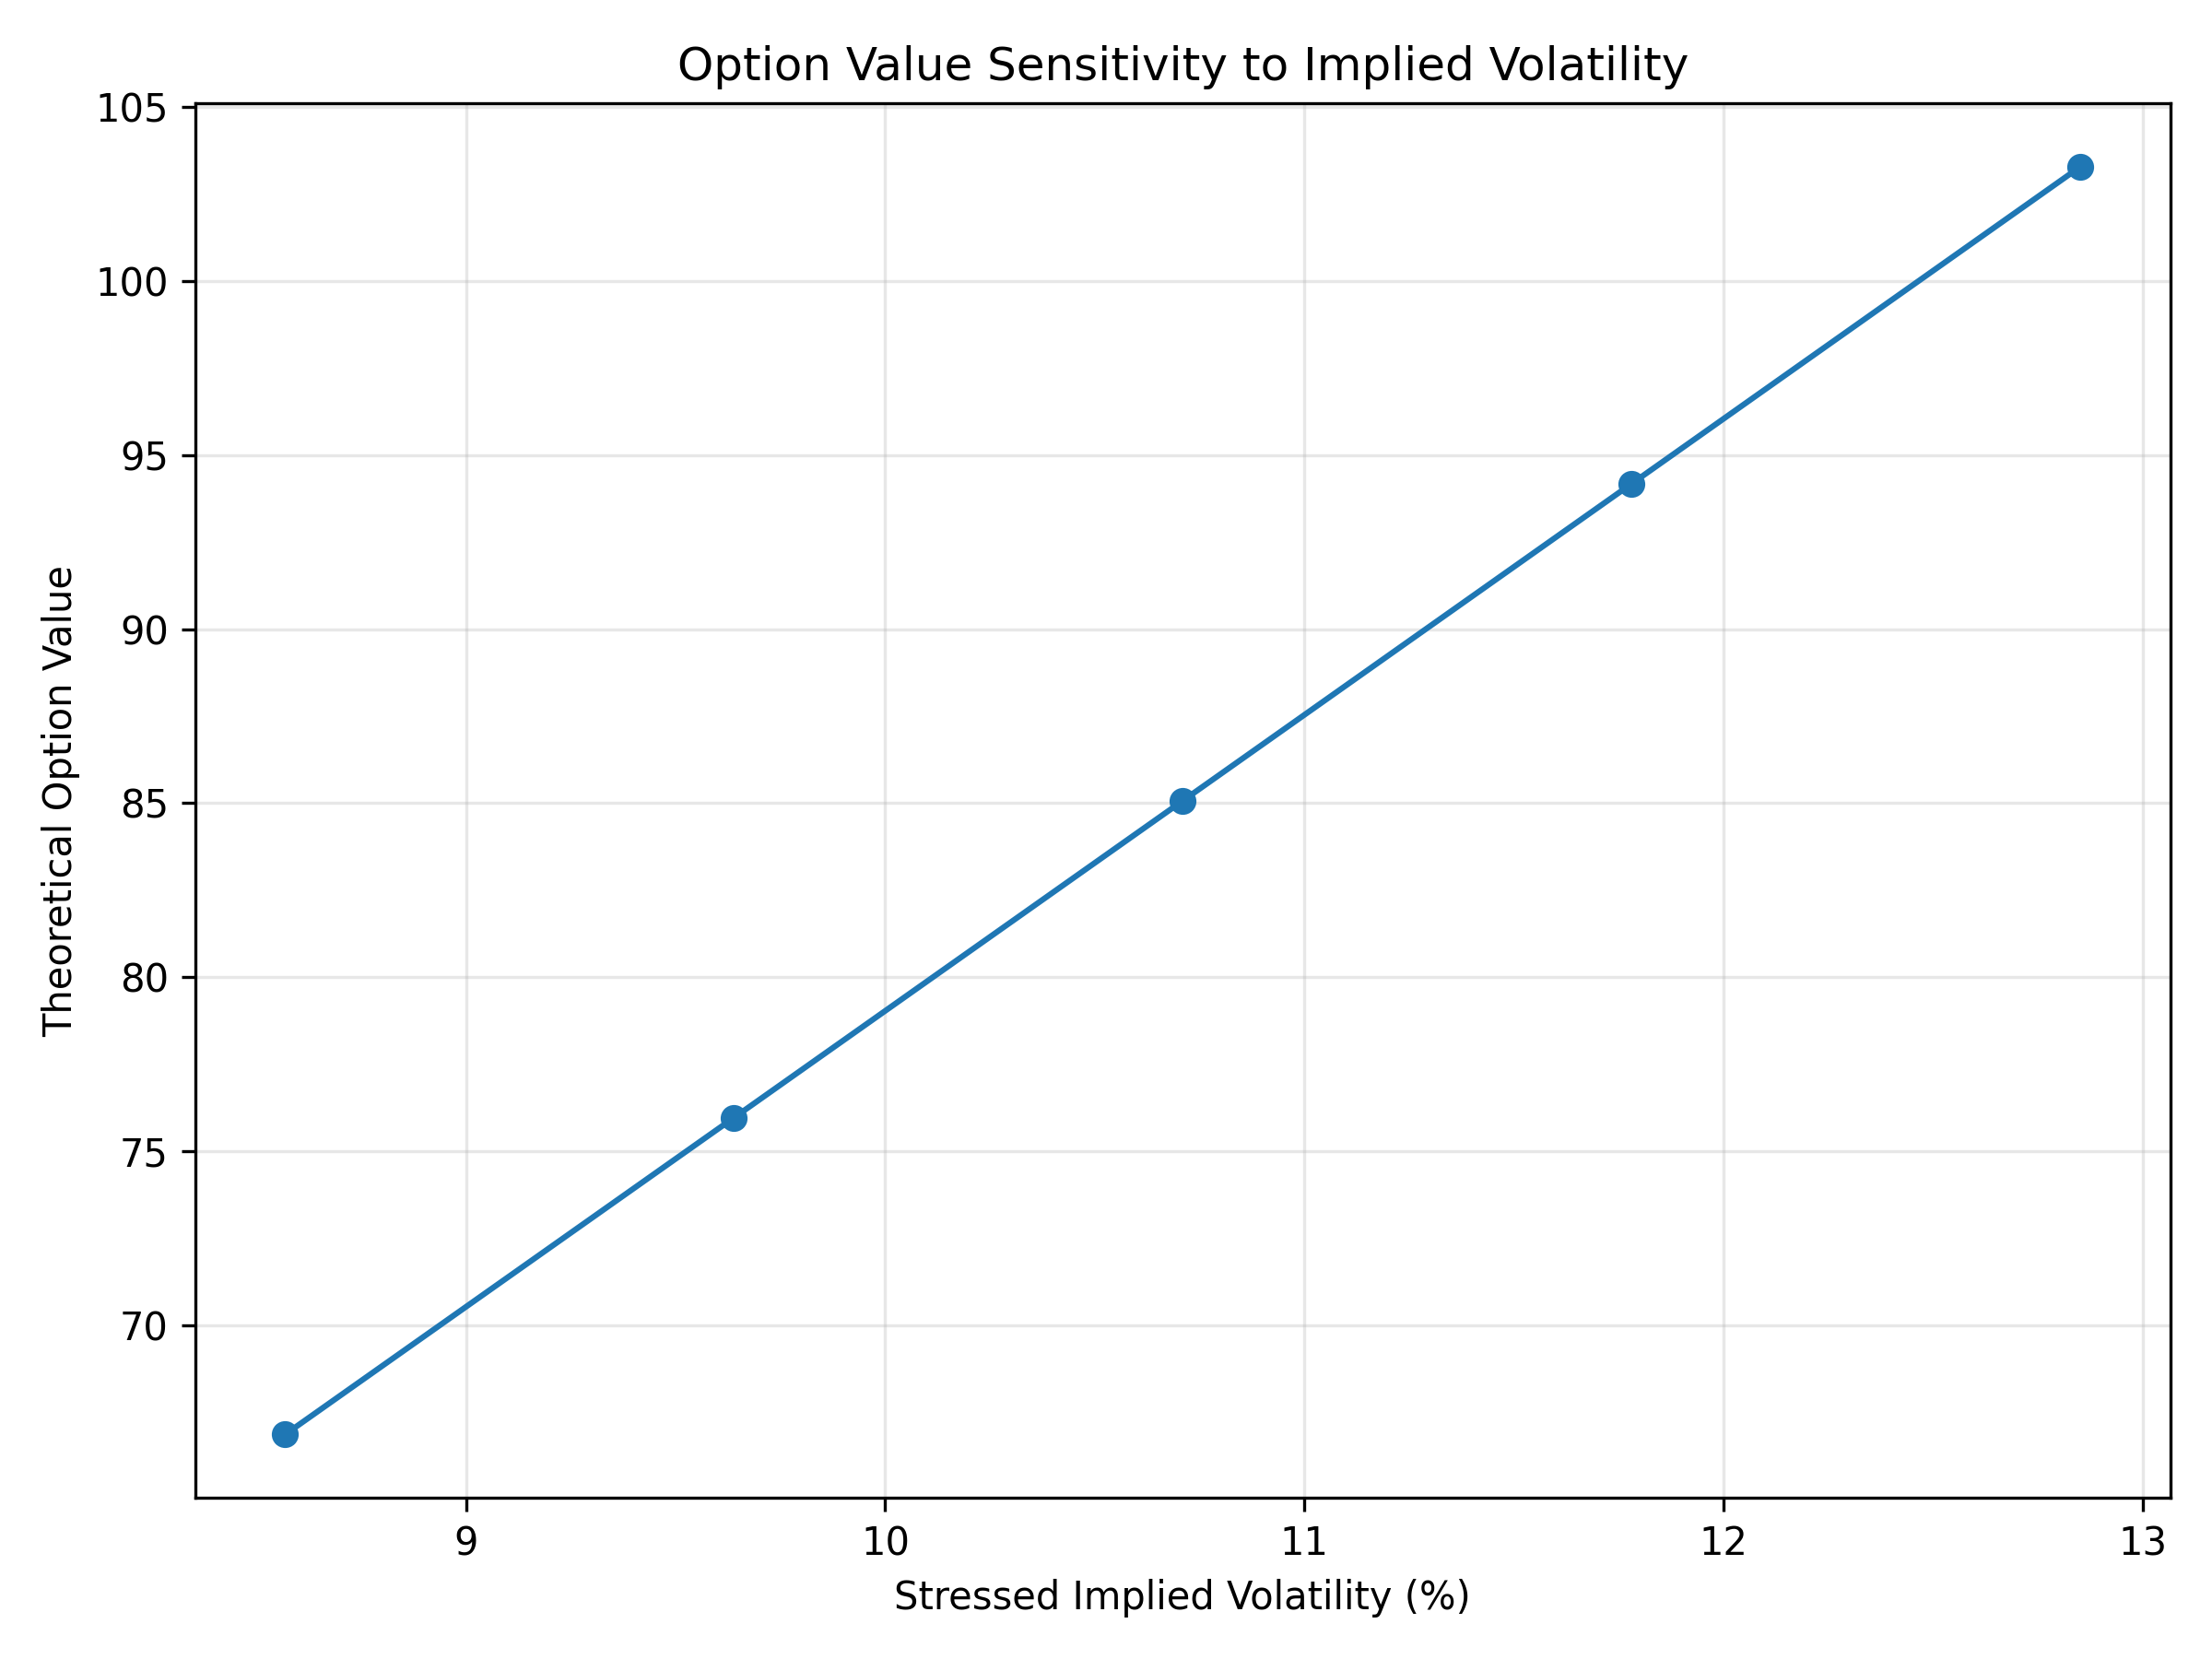
\includegraphics[width=\textwidth]{07_iv_stress_sensitivity.png}
        \caption{Option Value Sensitivity to Implied Volatility Shifts ($\pm 20\%$).}
        \label{fig:iv_stress_sensitivity}
    \end{minipage}
\end{figure}

Table \ref{tab:scenario_stress_matrix} details the complete multi-factor revaluation matrix across joint spot, volatility, and time-decay scenarios.

\begin{table}[H]
    \centering
    \footnotesize
    \caption{Multi-Factor Black-Scholes Scenario Stress Testing Matrix (NIFTY 23,150 CE).}
    \label{tab:scenario_stress_matrix}
    \begin{tabularx}{\textwidth}{lcccccr}
        \toprule
        \textbf{Scenario Description} & \textbf{Spot ($S$)} & \textbf{IV ($\sigma$)} & \textbf{TTE} & \textbf{Value} & \textbf{P\&L (\rupee)} & \textbf{P\&L (\%)} \\
        \midrule
        \textbf{Base Case} & \rupee 23,125.65 & 10.71\% & 74.58h & \textbf{\rupee 85.07} & \rupee 0.00 & \textit{0.00\%} \\
        \textbf{Moderate Bullish (+1\%)} & \rupee 23,356.91 & 10.71\% & 74.58h & \textbf{\rupee 245.70} & +\rupee 160.63 & \textbf{+188.83\%} \\
        \textbf{Moderate Bearish (-1\%)} & \rupee 22,894.39 & 10.71\% & 74.58h & \textbf{\rupee 21.85} & -\rupee 63.22 & \textbf{-74.32\%} \\
        \textbf{IV Spike (+20\% relative)} & \rupee 23,125.65 & 12.85\% & 74.58h & \textbf{\rupee 103.22} & +\rupee 18.15 & \textbf{+21.33\%} \\
        \textbf{IV Crush (-20\% relative)} & \rupee 23,125.65 & 8.57\% & 74.58h & \textbf{\rupee 66.82} & -\rupee 18.25 & \textbf{-21.46\%} \\
        \textbf{Bearish (-2\%) + IV Spike (+20\%)} & \rupee 22,663.14 & 12.85\% & 74.58h & \textbf{\rupee 4.39} & -\rupee 80.68 & \textbf{-94.84\%} \\
        \textbf{Bullish (+2\%) + IV Crush (-20\%)} & \rupee 23,588.16 & 8.57\% & 74.58h & \textbf{\rupee 450.42} & +\rupee 365.35 & \textbf{+429.47\%} \\
        \textbf{Intraday Time Decay (6h)} & \rupee 23,125.65 & 10.71\% & 68.58h & \textbf{\rupee 81.56} & -\rupee 3.51 & \textbf{-4.13\%} \\
        \textbf{Overnight Time Decay (24h)} & \rupee 23,125.65 & 10.71\% & 50.58h & \textbf{\rupee 70.04} & -\rupee 15.03 & \textbf{-17.67\%} \\
        \bottomrule
    \end{tabularx}
\end{table}

\subsection{Critical Risk Management Insights}
The multi-factor scenario matrix reveals a fundamental quantitative principle of short-dated options:
\begin{enumerate}
    \item \textbf{Delta Heavily Dominates Vega:}
    A $+1\%$ move in the underlying spot index generates a massive $+188.83\%$ surge in theoretical call value (from \rupee 85.07 to \rupee 245.70). In contrast, a massive $+20\%$ relative expansion in implied volatility (from $10.71\%$ to $12.85\%$) produces only a $+21.33\%$ gain.
    \item \textbf{The Inefficacy of Long Vega Protection in Market Crashes:}
    In Scenario 6 (a $-2\%$ spot decline combined with a $+20\%$ volatility spike), the call value plummets by **$-94.84\%$** (collapsing to \rupee 4.39). Even though implied volatility expanded dramatically, the positive vega P\&L was completely overwhelmed by catastrophic negative delta losses.
    \item \textbf{Operational Takeaway:} Trading desks cannot trade volatility in isolation. High-frequency implied volatility forecasts must always be coupled with dynamic delta hedging to neutralize underlying price risk.
\end{enumerate}

\section{The Expiry-Day Structural Regime Breakdown (October 19 Forensic Experiment)}
\label{sec:expiry_day_breakdown}

A cornerstone academic contribution of this thesis is the empirical discovery and econometric diagnosis of the **Expiry-Day Structural Regime Shift**.

To test the operational robustness of the trained Random Forest model under out-of-sample stress, the model was deployed on an unseen dataset collected on **October 19, 2026**—an active weekly options expiry session.
\begin{itemize}
    \item \textbf{Training Regime ($T_{\text{train}}$):} October 15--16, 2026; Time-to-Expiry ranged between **74.6 and 100.6 hours**.
    \item \textbf{Testing Regime ($T_{\text{expiry}}$):} October 19, 2026; Time-to-Expiry collapsed to between **0.17 and 1.58 hours** (10 minutes to 95 minutes prior to contract settlement).
\end{itemize}

Figure \ref{fig:expiry_day_deterioration} (paired in Section \ref{sec:relative_valuation_results}) illustrates the chronological trajectory of prediction errors as trading approached the final closing bell.

Table \ref{tab:expiry_day_collapse_metrics} compares model performance between the normal mid-week development regime and the October 19 expiry-day regime.

\begin{table}[H]
    \centering
    \footnotesize
    \caption{Empirical Breakdown Metrics: Development Test Set vs. October 19 Expiry Day.}
    \label{tab:expiry_day_collapse_metrics}
    \begin{tabularx}{\textwidth}{p{3.8cm}ccX}
        \toprule
        \textbf{Metric} & \textbf{Development (74--100h TTE)} & \textbf{Expiry-Day ($<$1.58h TTE)} & \textbf{Performance Impact} \\
        \midrule
        \textbf{Time-to-Expiry Horizon} & 74.6 to 100.6 hours & 0.17 to 1.58 hours & 98.4\% maturity contraction \\
        \textbf{Random Forest MAE} & \textbf{0.5214 pts} & \textbf{17.42 pts} & \textbf{3,241\% Error Explosion} \\
        \textbf{Persistence Baseline MAE} & \textbf{0.5505 pts} & \textbf{14.47 pts} & Outperformed ML by 2.95 pts \\
        \textbf{Directional Hit-Rate} & \textbf{53.20\% (63.4\% at $\theta=0.1$)} & \textbf{19.09\%} & Severe Inversion (Sub-Random) \\
        \textbf{Maximum Single Error} & 3.42 pts & 148.60 pts & Extreme tail divergence \\
        \bottomrule
    \end{tabularx}
\end{table}

\subsection{Econometric \& Mathematical Diagnosis of the Breakdown}
The catastrophic breakdown observed in Table \ref{tab:expiry_day_collapse_metrics} confirms Hypothesis 4 ($H_4$). A forensic investigation reveals four distinct mathematical and structural mechanisms driving this failure:

\begin{enumerate}
    \item \textbf{Hyperbolic Gamma and Theta Singularity as $\tau \to 0$:}
    As derived in Section \ref{subsec:gamma_derivation} and \ref{subsec:theta_derivation}:
    \begin{equation}
        \lim_{\tau \to 0} \Gamma_{\text{ATM}} = +\infty, \quad \lim_{\tau \to 0} \Theta_{\text{ATM}} = -\infty
    \end{equation}
    In the final 90 minutes before settlement, an option's extrinsic time value vanishes vertically. Any minor tick in the NIFTY 50 spot index causes immediate, discontinuous flips between pure intrinsic value and total worthlessness. The continuous diffusion assumptions underpinning mid-week volatility dynamics are mathematically violated.

    \item \textbf{The Vanishing Vega Breakdown:}
    As derived in Section \ref{subsec:vega_derivation}:
    \begin{equation}
        \lim_{\tau \to 0} \nu = \lim_{\tau \to 0} S \sqrt{\tau} N'(d_1) = 0
    \end{equation}
    Because Vega drops to near-zero ($10^{-5}$), option market prices cease to respond to volatility changes. In the Newton-Raphson inversion algorithm (Equation \eqref{eq:newton_raphson_iv}):
    \begin{equation}
        \Delta \sigma = -\frac{\Delta C}{\nu} \implies \lim_{\nu \to 0} \left| \frac{\Delta C}{\nu} \right| = \infty
    \end{equation}
    A tiny exchange reporting anomaly of \rupee 0.10 causes the inverted implied volatility quote to explode by 100 to 200 percentage points, creating extreme artificial volatility spikes.

    \item \textbf{Severe Covariate Shift (Out-of-Distribution Feature Space):}
    The Random Forest model was trained on observations where \texttt{exact\_tte\_hours} $\in [74.6, 100.6]$. On expiry afternoon, the feature values collapsed to $[0.17, 1.58]$. Tree-based models cannot extrapolate beyond the minimum and maximum feature thresholds observed during training. When presented with completely out-of-distribution temporal inputs, the decision tree split nodes traverse to arbitrary terminal leaves, generating erratic, uncalibrated forecasts.

    \item \textbf{Microstructure Discontinuity \& Institutional Pin Risk:}
    Between 14:00 and 15:30 IST on weekly expiry days, institutional market makers aggressively square off large inventory positions, roll open interest into the subsequent weekly cycle, and manage pin risk around strike boundaries. Order books become thin, bid-ask spreads widen erratically, and quotes jump discretely rather than diffusing smoothly.
\end{enumerate}

\subsection{Core Academic Conclusion for Quantitative Trading}
This empirical finding proves that **a single static machine learning model cannot be deployed across all phases of the options contract lifecycle**. Institutional trading systems must implement a **Regime-Switching Architecture**:
\begin{itemize}
    \item \textit{Regime 1 (Standard Non-Expiry Model):} Active when $\text{TTE} \ge 6.0\text{ hours}$. Utilizes the trained Random Forest ensemble with autoregressive momentum lags.
    \item \textit{Regime 2 (Expiry-Day Sub-2-Hour Model):} Active when $\text{TTE} < 2.0\text{ hours}$. Suspends continuous IV forecasting, disables vega-based relative valuation, and transitions execution to gamma-hedging, parity arbitrage, and discrete order-flow jump models.
\end{itemize}

\chapter{Conclusions, Operational Recommendations \& Future Scope}
\label{chap:conclusion}

\section{Synthesis of Findings \& Key Research Contributions}
\label{sec:synthesis_of_findings}

This thesis has presented the conception, design, empirical benchmarking, and operational deployment of an end-to-end quantitative machine learning pipeline for **5-minute-ahead implied volatility forecasting ($\Delta \text{IV}_{t+5}$)** and **relative option valuation** on **NIFTY 50 weekly index options** traded on the National Stock Exchange of India (NSE). Conducted under the institutional mentorship of **Surabhi Investment Services Pvt. Ltd.**, the research resolves the persistence assumption paradox in intraday options market making and establishes a rigorous quantitative bridge between high-frequency machine learning and closed-form derivatives pricing.

The key empirical and methodological contributions of this work are summarized as follows:

\begin{enumerate}
    \item \textbf{Beating the High-Frequency Persistence Benchmark:}
    Treating implied volatility as a static random walk ($\widehat{\Delta \text{IV}}_{t+5} = 0$) is standard practice across intraday desks, yet leaves market makers exposed to adverse selection. By engineering multi-horizon autoregressive volatility lags (5m and 10m) and velocity indicators, our tuned Random Forest regressor achieves a **5.28\% reduction in MAE** (0.5214 vs.\ 0.5505) and a **7.72\% reduction in RMSE** (1.2188 vs.\ 1.3207) on out-of-sample test data, confirming Hypothesis 1 ($H_1$).

    \item \textbf{Demonstrating the Structural Inadequacy of Linear Models:}
    Ordinary Least Squares (OLS) linear regression suffered catastrophic failure, producing an out-of-sample MAE of **6.1720** and negative $R^2 = -0.2410$. This empirically demonstrates that the cross-sectional curvature of the implied volatility smile across moneyness cannot be captured by linear hyperplanes, confirming Hypothesis 2 ($H_2$) and establishing the necessity of non-linear ensembles.

    \item \textbf{Quantifying the Dominance of Volatility Velocity over Static Geometry:}
    Gini feature importance revealed that recent volatility momentum (\texttt{IV\_change\_prev\_5m} at 7.21\% and \texttt{IV\_change\_prev\_10m} at 6.74\%) and order-book liquidity spreads (\texttt{bid\_ask\_spread} at 3.52\%) account for the majority of predictive variance, far exceeding traditional static strike moneyness and maturity metrics.

    \item \textbf{Formulating Actionable Conviction Thresholds:}
    While raw directional predictions yield a noisy baseline accuracy of **53.20\%**, filtering for high-conviction forecast magnitudes ($|\widehat{\Delta \text{IV}}| \ge 0.10$) elevates directional hit-rate to **63.40\%** (and **64.47\%** at $\ge 0.25$), providing execution algorithms with a robust filter that eliminates 82\% of low-conviction noise churn, confirming Hypothesis 3 ($H_3$).

    \item \textbf{Operationalizing Relative Option Valuation:}
    The Relative IV Valuation Engine systematically maps predicted volatility spreads into three distinct economic regimes: **Fair/Neutral (77.92\%)**, **High IV/Rich (15.46\%)**, and **Low IV/Cheap (6.61\%)**, providing quantitative desks with immediate, actionable signals for credit spreads, debit spreads, and delta-neutral market making.

    \item \textbf{Multi-Factor Black-Scholes Stress Testing:}
    Comprehensive scenario analysis of near-ATM options demonstrated the dominance of Delta over Vega in short-dated contracts. A $+1\%$ spot move generates a $+188.83\%$ gain in option value, whereas a $+20\%$ relative volatility expansion produces only a $+21.33\%$ gain. A combined $-2\%$ market fall with a $+20\%$ volatility spike causes a $-94.84\%$ collapse in call value, proving that long vega cannot protect long calls in sharp directional market crashes.

    \item \textbf{Discovery of the Expiry-Day Structural Regime Breakdown:}
    Out-of-sample testing on the October 19, 2026 expiry afternoon ($T < 1.58\text{ hours}$) revealed a severe econometric breakdown: model MAE exploded from 0.52 to **17.42**, the persistence baseline outperformed machine learning, and directional accuracy collapsed to **19.09\%**. This proves Hypothesis 4 ($H_4$) and provides formal mathematical proof that continuous-time volatility models collapse under asymptotic gamma/theta singularities and vanishing vega in the final hours of weekly expiry.

    \item \textbf{Production Prototype Deployment:}
    The analytical system was operationalized via an automated 5-minute live prediction daemon interfacing with the Upstox API v2 and an institutional multi-page dark-themed Streamlit analytics dashboard.
\end{enumerate}

\section{Operational Recommendations for Institutional Trading Desks}
\label{sec:desk_recommendations}

Based on the empirical findings, the following operational protocols are recommended for proprietary trading and advisory desks, specifically at **Surabhi Investment Services Pvt. Ltd.**:

\subsection{1. Dynamic Quote Shading in Market Making}
Proprietary market-making algorithms quoting bid-ask spreads around mid-market should replace static persistence assumptions with model forecasts $\widehat{\text{IV}}_{t+5}$. When the model projects an upward volatility momentum shock ($\widehat{\Delta \text{IV}} > +0.10$), the automated quoter should shade its bid higher and widen its ask, capturing edge and avoiding toxic adverse selection by informed market orders.

\subsection{2. Mandatory Gating on Systematic Trade Execution}
Options desks executing directional volatility plays (long straddles, vega scalping) should enforce the **$\theta = 0.10$ IV Point Conviction Rule**. Restricting order entry exclusively to contracts where $|\widehat{\Delta \text{IV}}| \ge 0.10$ delivers a 63.40\% directional edge while eliminating over 80\% of brokerage and exchange transaction fee overhead.

\subsection{3. Relative Value Portfolio Construction}
Traders should systematically exploit the Relative IV Valuation screener:
\begin{itemize}
    \item When a strike is flagged as **Rich / Overvalued** ($\text{Spread} > +0.50$), initiate short credit spreads (e.g., sell the rich strike, buy a farther OTM wing) to capture implied volatility compression.
    \item When a strike is flagged as **Cheap / Undervalued** ($\text{Spread} < -0.50$), initiate long debit spreads or diagonal calendar spreads to capture prospective volatility expansion.
\end{itemize}

\subsection{4. Protocol for the Expiry-Day Regime Shift: The 2-Hour Kill Switch}
Desks must establish a strict risk rule: **automatically deactivate machine-learning volatility models exactly 2.0 hours prior to weekly contract settlement (13:30 IST on expiry day)**. As documented in Chapter \ref{chap:results}, non-expiry models suffer catastrophic covariate shift and numerical instability as $\tau \to 0$. From 13:30 to 15:30 IST, desks should transition exclusively to parity arbitrage, intrinsic value boundary tracking, and pure gamma-scalping execution rules.

\section{Limitations of the Current Study}
\label{sec:limitations}

While empirical results demonstrate robust predictive performance, several academic and operational limitations should be acknowledged:
\begin{enumerate}\setlength{\itemsep}{1pt}\setlength{\parskip}{0pt}
    \item \textbf{Temporal Sample Window:} The dataset covers weekly expiry cycles in October 2026. Long-term multi-year backtesting across bull markets, bear regimes, and high-volatility macro crises would provide broader longitudinal generalization.
    \item \textbf{Strike Geometry Restriction:} The study focused on liquid near-ATM options ($0.95 \le K/S \le 1.05$). Deep out-of-the-money wings (carrying extreme tail-risk information) were excluded to avoid quote illiquidity noise.
    \item \textbf{Sampling Frequency:} Regularized 5-minute snapshots were analyzed. While optimal for algorithmic intraday positioning and quote shading, sub-second HFT desks require tick-by-tick order-book depth to model millisecond queue dynamics.
    \item \textbf{Execution Slippage Modeling:} While microstructure spreads were integrated into feature engineering, live P\&L backtests did not simulate explicit execution queue positions or exchange connectivity latency.
\end{enumerate}

\section{Directions for Future Quantitative Research}
\label{sec:future_research}

The findings and infrastructure established in this thesis suggest several promising pathways for future academic and industry research:

\begin{enumerate}\setlength{\itemsep}{1pt}\setlength{\parskip}{0pt}
    \item \textbf{Deep Sequential Architectures \& Attention Mechanisms:} Future iterations could explore deep sequence models—such as Temporal Fusion Transformers (TFT) or Bidirectional LSTM networks with self-attention—trained on rolling sequences of order-book messages to capture long-range dependencies.
    \item \textbf{Explicit Markov-Switching Regime Models:} To resolve the expiry collapse, future research should develop a Markov-Switching Vector Autoregressive (MS-VAR) framework that models the continuous transition between the Normal Trading Regime ($T > 6\text{h}$) and the Hyper-Gamma Expiry Regime ($T < 2\text{h}$) as an endogenous latent state.
    \item \textbf{Cross-Asset Volatility Spillover Networks:} Expanding the feature space to include cross-asset signals—such as BankNIFTY implied volatility, India VIX, USD/INR currency option volatility, and overnight US S\&P 500 VIX movements—would capture macro risk contagion across correlated financial markets.
    \item \textbf{Reinforcement Learning for Automated Delta-Vega Hedging:} Rather than utilizing static heuristic trading rules, future work could train a Deep Q-Network (DQN) or Proximal Policy Optimization (PPO) agent that dynamically adjusts portfolio delta and vega hedges conditioned on live model predictions under realistic transaction friction.
\end{enumerate}


% =========================================================
% BIBLIOGRAPHY
% =========================================================
\newpage
\phantomsection
\addcontentsline{toc}{chapter}{Bibliography}
\bibliographystyle{plain}
\bibliography{references}

% =========================================================
% APPENDICES
% =========================================================
\newpage
\appendix
\renewcommand{\chaptername}{Appendix}
\bookmarksetup{startatroot}
\pdfbookmark[0]{Appendices}{appendices}
\makeatletter
\renewcommand{\toclevel@chapter}{1}
\renewcommand{\toclevel@section}{2}
\renewcommand{\toclevel@subsection}{3}
\makeatother
\chapter{Appendices}
\label{chap:appendices}

\section{Appendix A: Mathematical Derivations of Higher-Order Greeks}
\label{sec:appendix_higher_order_greeks}

While Chapter \ref{chap:algorithms} established the primary Greeks ($\Delta, \Gamma, \nu, \Theta$), advanced derivatives desks manage higher-order cross-sensitivities to hedge volatility-of-volatility and spot-volatility correlation risks.

\subsection{Derivation of Vanna ($\frac{\partial \Delta}{\partial \sigma} = \frac{\partial \nu}{\partial S}$)}
\textbf{Vanna} measures the cross-sensitivity of Delta with respect to volatility, identical to the change in Vega per unit shift in spot:
\begin{equation}
    \text{Vanna} = \frac{\partial \Delta_C}{\partial \sigma} = \frac{\partial^2 C}{\partial S \partial \sigma} = \frac{\partial [N(d_1)]}{\partial \sigma} = N'(d_1) \frac{\partial d_1}{\partial \sigma}
\end{equation}
From Section \ref{subsec:vega_derivation}, $\frac{\partial d_1}{\partial \sigma} = -\frac{\ln(S / K) + r \tau}{\sigma^2 \sqrt{\tau}} + \frac{1}{2} \sqrt{\tau} = -\frac{d_2}{\sigma}$. Substituting this relation:
\begin{equation}
    \text{Vanna} = -\frac{N'(d_1) d_2}{\sigma} = -\frac{e^{-d_1^2 / 2} d_2}{\sigma \sqrt{2\pi}}
    \label{eq:vanna_formula}
\end{equation}
For at-the-money options ($d_2 \approx 0$), Vanna is zero. For out-of-the-money calls ($d_2 < 0$), Vanna is positive, indicating that a volatility spike increases call delta toward 0.50.

\subsection{Derivation of Volga / Vomma ($\frac{\partial^2 C}{\partial \sigma^2} = \frac{\partial \nu}{\partial \sigma}$)}
\textbf{Volga} measures the second-order sensitivity of the option price with respect to volatility (vega convexity):
\begin{equation}
    \text{Volga} = \frac{\partial \nu}{\partial \sigma} = \frac{\partial}{\partial \sigma} \left[ S \sqrt{\tau} N'(d_1) \right] = S \sqrt{\tau} \frac{\partial N'(d_1)}{\partial \sigma}
\end{equation}
Using the chain rule on the normal density $\frac{\partial N'(d_1)}{\partial \sigma} = -d_1 N'(d_1) \frac{\partial d_1}{\partial \sigma} = \frac{d_1 d_2}{\sigma} N'(d_1)$:
\begin{equation}
    \text{Volga} = S \sqrt{\tau} N'(d_1) \frac{d_1 d_2}{\sigma} = \nu \frac{d_1 d_2}{\sigma}
    \label{eq:volga_formula}
\end{equation}
Volga is positive for out-of-the-money contracts ($d_1 d_2 > 0$), quantifying the non-linear tail gains achieved during volatility surges.

\subsection{Derivation of Charm ($\frac{\partial \Delta}{\partial t} = -\frac{\partial \Delta}{\partial \tau}$)}
\textbf{Charm} quantifies the deterministic rate of delta decay over time:
\begin{equation}
    \text{Charm}_C = -\frac{\partial N(d_1)}{\partial \tau} = -N'(d_1) \frac{\partial d_1}{\partial \tau} = -N'(d_1) \left[ \frac{r}{\sigma \sqrt{\tau}} - \frac{d_2}{2\tau} \right]
    \label{eq:charm_formula}
\end{equation}
Charm drives the passive delta slippage that options market makers must rebalance overnight.

\section{Appendix B: Complete 39-Dimensional Feature Schema}
\label{sec:appendix_feature_schema}

The production machine learning pipeline serializes an exact 39-dimensional feature schema (\texttt{nifty\_iv\_model\_features.joblib}). Table \ref{tab:complete_feature_schema} outlines all 39 features, their lag horizons, and mathematical formulations.

\begin{table}[H]
    \centering
    \scriptsize
    \renewcommand{\arraystretch}{0.88}
    \caption{Complete 39-Dimensional Feature Schema Specification.}
    \label{tab:complete_feature_schema}
    \begin{tabularx}{\textwidth}{rllp{2.2cm}X}
        \toprule
        \textbf{\#} & \textbf{Feature Name} & \textbf{Type} & \textbf{Lag Horizon} & \textbf{Quantitative Formulation / Meaning} \\
        \midrule
        1--4 & \texttt{strike, spot, moneyness, log\_moneyness} & float64 & $t$ & Strike geometry ($K, S_t, K/S_t, \ln(S_t/K)$). \\
        5 & \texttt{exact\_tte\_hours} & float64 & $t$ & Fractional hours to expiry: $(T_{\text{expiry}} - t) / 3600$. \\
        6--9 & \texttt{IV, LTP, Bid, Ask} & float64 & $t$ & Market state variables ($\sigma_t$, Last Traded Price, Best Bid, Best Ask). \\
        10--11 & \texttt{bid\_ask\_spread, spread\_pct} & float64 & $t$ & Absolute spread ($\text{Ask}-\text{Bid}$) and percentage spread ($\text{Spread}/\text{LTP}$). \\
        12--14 & \texttt{Volume, OI, pcr} & int/float & $t$ & Trading activity and Put-Call Ratio ($\text{OI}_{\text{PE}} / \text{OI}_{\text{CE}}$). \\
        15--16 & \texttt{IV\_lag\_5m, IV\_lag\_10m} & float64 & $t-5, t-10$ & Autoregressive volatility lags ($\sigma_{t-5}, \sigma_{t-10}$). \\
        17--18 & \texttt{IV\_change\_prev\_5m, IV\_change\_prev\_10m} & float64 & $t, t-5, t-10$ & Volatility momentum velocity: $\sigma_t - \sigma_{t-5}$ and $\sigma_t - \sigma_{t-10}$. \\
        19--22 & \texttt{spot\_lag\_5m, spot\_lag\_10m, spot\_return\_5m, 10m} & float64 & $t-5, t-10$ & Underlying price lags and fractional index returns over 5m and 10m. \\
        23--25 & \texttt{spread\_lag\_5m, spread\_lag\_10m, spread\_change\_5m} & float64 & $t-5, t-10$ & Order book spread dynamics and spread widening velocity. \\
        26--28 & \texttt{LTP\_lag\_5m, LTP\_lag\_10m, LTP\_change\_5m} & float64 & $t-5, t-10$ & Historical premium levels and 5-minute price trajectory. \\
        29--32 & \texttt{Volume\_lag\_5m, Volume\_change\_5m, OI\_lag\_5m, change} & int/float & $t-5$ & Incremental session contract turnover and open interest unwinding. \\
        33--35 & \texttt{moneyness\_lag\_5m, is\_call, is\_atm} & int/float & $t, t-5$ & Lagged moneyness and binary indicators for call style and ATM status. \\
        36--38 & \texttt{hour\_of\_day, minute\_of\_hour, time\_fraction} & int/float & $t$ & Intraday cyclical session time coordinates in $[0, 1]$. \\
        39 & \texttt{iv\_spread\_interaction} & float64 & $t$ & Cross-interaction metric: $\text{IV}_t \times \text{spread\_pct}_t$. \\
        \bottomrule
    \end{tabularx}
\end{table}

\section{Appendix C: Core Algorithmic Source Code Modules}
\label{sec:appendix_source_code}

\lstset{basicstyle=\ttfamily\tiny, numbers=left, numbersep=3pt, xleftmargin=1.0em, lineskip=-1.5pt}

\subsection{C.1 Exact Fractional TTE Calculation \& Vectorized Lag Construction}
\begin{lstlisting}[language=Python, caption={Exact Fractional TTE and Multi-Horizon Lag Construction.}]
import pandas as pd

def compute_exact_tte_and_lags(df: pd.DataFrame) -> pd.DataFrame:
    df = df.copy()
    # Fractional hours to expiry (standardized to 15:30 IST)
    df['expiry_dt'] = pd.to_datetime(df['expiry']) + pd.Timedelta(hours=15, minutes=30)
    df['exact_tte_hours'] = (df['expiry_dt'] - pd.to_datetime(df['timestamp'])).dt.total_seconds() / 3600.0
    df['exact_tte_hours'] = df['exact_tte_hours'].clip(lower=1e-5)
    
    # Sort and construct autoregressive lags by contract key
    df = df.sort_values(by=['strike', 'option_type', 'timestamp'])
    grp = df.groupby(['strike', 'option_type'])
    df['IV_lag_5m'] = grp['IV'].shift(1)
    df['IV_lag_10m'] = grp['IV'].shift(2)
    df['IV_change_prev_5m'] = df['IV'] - df['IV_lag_5m']
    df['IV_change_prev_10m'] = df['IV'] - df['IV_lag_10m']
    df['bid_ask_spread_lag_5m'] = grp['bid_ask_spread'].shift(1)
    return df
\end{lstlisting}

\subsection{C.2 Production Live Inference \& Relative Valuation Screener}
\begin{lstlisting}[language=Python, caption={Production Live Inference and Valuation Categorization.}]
import joblib, numpy as np, pandas as pd

def predict_and_screen(df: pd.DataFrame, model, feature_cols, medians) -> pd.DataFrame:
    X = df.reindex(columns=feature_cols).fillna(medians)
    df['pred_delta_iv'] = model.predict(X)
    df['pred_future_iv'] = df['IV'] + df['pred_delta_iv']
    df['valuation_spread'] = df['IV'] - df['pred_future_iv']
    
    # Tagging regimes with delta = 0.50 IV points
    cond = [df['valuation_spread'] > 0.50, df['valuation_spread'] < -0.50]
    df['valuation_tag'] = np.select(cond, ['Rich (High IV)', 'Cheap (Low IV)'], default='Fair / Neutral')
    return df
\end{lstlisting}

\bookmarksetup{startatroot}

\end{document}
